%%%%
%% Load the class. Put any options that you want here (see the documentation
%% for the list of options). The following are samples for each type of
%% thesis:
%%
%% Note: you can also specify any of the following options:
%%  logo: put a University of Edinburgh logo onto the title page
%%  frontabs: put the abstract onto the title page
%%  deptreport: produce a title page that fits into a Computer Science
%%      departmental cover [not sure if this actually works]
%%  singlespacing, fullspacing, doublespacing: choose line spacing
%%  oneside, twoside: specify a one-sided or two-sided thesis
%%  10pt, 11pt, 12pt: choose a font size
%%  centrechapter, leftchapter, rightchapter: alignment of chapter headings
%%  sansheadings, normalheadings: headings and captions in sans-serif
%%      (default) or in the same font as the rest of the thesis
%%  [no]listsintoc: put list of figures/tables in table of contents (default:
%%      not)
%%  romanprepages, plainprepages: number the preliminary pages with Roman
%%      numerals (default) or consecutively with the rest of the thesis
%%  parskip: don't indent paragraphs, put a blank line between instead
%%  abbrevs: define a list of useful abbreviations (see documentation)
%%  draft: produce a single-spaced, double-sided thesis with narrow margins
%%
%% For a PhD thesis -- you must also specify a research institute:
\documentclass[phd,aiai,twoside]{infthesis}

\usepackage{hyperref}
\usepackage[table]{xcolor}
\usepackage[ruled,vlined,linesnumbered]{algorithm2e}
\usepackage{amssymb}
\usepackage{amsthm}
\usepackage{mathtools}
\usepackage[capitalise]{cleveref}
\usepackage{tikz}
\usepackage{mathrsfs}
\usepackage[nounderscore]{syntax}
\usepackage{blkarray}
\usepackage[binary-units]{siunitx}
\usepackage[inline,shortlabels]{enumitem}
\usepackage{capt-of}
%\usepackage[caption=false]{subfig}
\usepackage{booktabs}
\usepackage[misc,geometry]{ifsym}
\usepackage{breakcites}
\usepackage[british]{babel}
\usepackage{natbib}
\usepackage{complexity}
\usepackage{multirow}
\usepackage{amsfonts}
\usepackage{subcaption}
\usepackage{graphicx}
\usepackage{sectsty}

\allsectionsfont{\raggedright}

\usetikzlibrary{arrows.meta}
\captionsetup[subfigure]{width=\linewidth}

\newtheorem{constraint}{Constraint}
\newtheorem{proposition}{Proposition}
\newtheorem{theorem}{Theorem}
\newtheorem{lemma}{Lemma}
\theoremstyle{definition}
\newtheorem{definition}{Definition}
\newtheorem{example}{Example}
\theoremstyle{remark}
\newtheorem*{remark}{Remark}

\renewcommand\fbox{\fcolorbox{red}{white}}
\newcommand{\hilight}[1]{\setlength{\fboxsep}{1pt}\colorbox{lightgray}{#1}}
\newcommand{\hlitem}{\stepcounter{enumi}\item[\hilight{\theenumi}]}

\newcommand{\logical}[1]{{\normalfont \texttt{#1}}}
\newcommand{\variable}[1]{\texttt{\textup{#1}}}
\newcommand{\arrayd}[3]{\variable{{#1}[}{#2}\variable{]} \in {#3}}
% 1=name, 2=length, 3=type
\newcommand{\arrayt}[3]{\variable{{#3}} : \variable{{#1}[}{#2}\variable{]}}

\newcommand{\predicates}{\mathcal{P}}
\newcommand{\variables}{\mathcal{V}}
\newcommand{\constants}{\mathcal{C}}
\newcommand{\tokens}{\mathcal{T}}
\newcommand{\arities}{\mathcal{A}}
\newcommand{\maxArity}{\mathcal{M}_{\mathcal{A}}}
\newcommand{\maxNumNodes}{\mathcal{M}_{\mathcal{N}}}
\newcommand{\maxNumClauses}{\mathcal{M}_{\mathcal{C}}}

\DeclareMathOperator{\Determined}{\Delta}
\DeclareMathOperator{\Undetermined}{\Upsilon}
\DeclareMathOperator{\AlmostDetermined}{\Gamma}
\DeclareMathOperator{\getss}{\mathtt{:-}}
\DeclareMathOperator{\im}{im}

\Crefname{algocf}{Algorithm}{Algorithms}
\Crefname{constraint}{Constraint}{Constraints}
\crefname{section}{Sect.}{Sects.}

\makeatletter
\newcommand{\nosemic}{\renewcommand{\@endalgocfline}{\relax}}% Drop semi-colon ;
\newcommand{\dosemic}{\renewcommand{\@endalgocfline}{\algocf@endline}}% Reinstate semi-colon ;
\newcommand{\pushline}{\Indp}% Indent
\newcommand{\popline}{\Indm\dosemic}% Undent
\makeatother

\newtheorem{innercustomthm}{Theorem}
\newenvironment{customthm}[1]
               {\renewcommand\theinnercustomthm{#1}\innercustomthm}
               {\endinnercustomthm}
               \newtheorem{innercustomlemma}{Lemma}
               \newenvironment{customlemma}[1]
                              {\renewcommand\theinnercustomlemma{#1}\innercustomlemma}
                              {\endinnercustomlemma}

\crefname{enumi}{Condition}{Conditions}
\crefname{enumii}{Condition}{Conditions}

\title{Probabilistic Inference via Weighted Model Counting: Algorithms, Encodings, and Random Instances}
\author{Paulius Dilkas}

\abstract{%
  This doctoral thesis will present the results of my work into the
  reanimation of lifeless human tissues.
}

\begin{document}

\begin{preliminary}

\maketitle

\begin{acknowledgements}
  Many thanks to my mummy for the numerous packed lunches; and of course to Igor, my faithful lab assistant.

  The first author was supported by the EPSRC Centre for Doctoral Training in Robotics and Autonomous Systems, funded by the UK Engineering and Physical Sciences Research Council (grant EP/L016834/1). This work has made use of the resources provided by the Edinburgh Compute and Data Facility (ECDF) (\url{http://www.ecdf.ed.ac.uk/}).

  We thank the anonymous reviewers for their helpful comments.
\end{acknowledgements}

\standarddeclaration

%% Finally, a dedication (this is optional -- uncomment the following line if
%% you want one).
% \dedication{To my mummy.}

\tableofcontents

%% If you want a list of figures or tables, uncomment the appropriate line(s)
% \listoffigures
% \listoftables

\end{preliminary}

% TODO:
% * Some citations appear as Author [year] in the first chapter.
% * Alignment issues.
% * Consider removing all the subfigure/minipage/subfig stuff.
% * Fix references to not use the 'proceedings' command.
% * make sure all table captions are above (?) the table

%% where does my work fit in?
%% how would I explain my work to a layman?
%% emphasise timeliness, i.e., why now? Because ADDMC allows for my ideas to become implementable.
%% why I chose to work on what I did
%% why these gaps are the ones to be filled (at this time)
%% emphasise methodological contributions
%% mindset:
%% * generalise everything
%% * implement a solution that works well in practice
%% * use both theoretical and experimental methods to understand why it works
%% why the reader should find this work interesting AND how the current state of research led me to work on my RQ
%% why, what, and how

%% motivation (context)
%% (related efforts)
%% problem formulation
%% research objectives
%% research questions
%% contributions

% broad goal -> objectives -> another specific area -> the problem -> specifics

\chapter{Introduction} % 5-14 pages (9 on average)

% ==================== WMC====================

% * probabilistic inference
% * TODO: specific examples of the kind of problems that are being solved by WMC/WFOMC?
% * WMC algorithms (TODO: copy some info from my review)
% * More generally...
% ** WMC and WFOMC
% ** sum-of-product problems

\begin{table}
  \caption{An assortment of problems that require one to compute a quantity defined as a sum of products.}
  \label{table:comparison}
  \centering
  \begin{tabular}{lll}
    \toprule
    Problem & Sum/Integral (over) & Product (over) \\
    \midrule
    WMC & models of a propositional theory & literals \\
    PBP & models of a propositional theory & arbitrary \\
    SP & models of a propositional theory & arbitrary \\
    WMI & models of a propositional LRA theory & literals \\
    WFOMC & models of a first-order theory & predicates \\
    WFOMI & models of a first-order LRA theory & predicates \\
    SumProd & instantiations of discrete variables & functions \\
    Algebraic path & paths in a graph & edges in a path \\
    Permanent & permutations & elements of a matrix \\
    \bottomrule
  \end{tabular}
\end{table}

\begin{itemize}
\item weighted model counting (WMC) \citep{DBLP:journals/ai/ChaviraD08}
\item pseudo-Boolean projection (PBP) (\cref{chapter:wmc2})
\item semiring programming (SP) \citep{DBLP:journals/ijar/BelleR20}
\item weighted model integration (WMI) \citep{DBLP:conf/ijcai/BellePB15}
\item weighted (symmetric) first-order model counting (WFOMC) \citep{DBLP:conf/ijcai/BroeckTMDR11}
\item weighted (symmetric) first-order model integration \citep{DBLP:conf/uai/FeldsteinB21}
\item SumProd \citep{DBLP:journals/ai/Dechter99,DBLP:journals/jair/BacchusDP09}
\item the algebraic path problem \citep{DBLP:series/synthesis/2010Baras}
\item computing the permanent \citep{DBLP:journals/tcs/Valiant79}
\end{itemize}

Despite the variety of representations, probabilistic inference (via WMC and
otherwise, more on this in the next section) can be seen as a single
computational problem. Thus, it is all the more important to develop WMC
algorithms with good empirical performance, understand the comparative strengths
and weaknesses of different approaches, and optimise the encoding process that
transforms the initial representation of a probability distribution to a
representation accepted by the algorithm. In my work, I address this problem by
assessing the empirical performance of these algorithms on random instances of
different kinds, revealing the weaknesses of the standard definition of WMC, and
suggesting more expressive alternatives.

% ==================== My approach: generalisation ====================

Examples of generalisation
\begin{itemize}
\item resolution vs cutting planes in SAT (i.e., CNF vs PB)
\item SAT/CSP/LP/IP vs algorithms to specific combinatorial problems
\item Einstein (general relativity) vs Newton (gravity)
\item category theory vs algebra/topology/algebraic topology
\end{itemize}

Two ideas:
\begin{itemize}
\item Manipulating more expressive representations can lead to more
  efficient algorithms (c.f., cutting planes vs. resolution in SAT).
\item Random problem instances can help reveal fundamental differences in
  how algorithms behave in practice.
\end{itemize}

\section{Contributions and Outline} % 2 pages

\begin{figure}[t]
  \centering
  \begin{tikzpicture}[node distance=2.5cm]
    \node[draw,ultra thick,color=gray,text=black] (cp) {Constraint programming};
    \node[draw,ultra thick,right=0.5cm of cp,color=gray,text=black] (random) {Random algorithms};

    \node[draw,ultra thick,color=gray,below=1cm of cp,text=black] (bn) {Bayesian networks};
    \node[draw,ultra thick,right=0.5cm of bn,color=gray,text=black] (problog) {ProbLog};
    \node[draw,ultra thick,right=0.5cm of problog,color=gray,text=black] (mln) {Markov logic};

    \node[draw,ultra thick,below=1cm of bn,color=wmc2,text=black] (pbp) {PBP};
    \node[draw,ultra thick,below=1cm of problog,color=wmc1,text=black] (wmc) {WMC};
    \node[draw,ultra thick,below=1cm of mln,color=gray,text=black] (wfomc) {WFOMC};

    \node[draw,ultra thick,below=1cm of pbp,color=comparison,text=black] (dpmc) {DPMC};
    \node[draw,ultra thick,color=comparison,text=black,left of=dpmc] (addmc) {ADDMC};
    \node[draw,ultra thick,below=1cm of wmc,color=comparison,text=black,text width=1.85cm,align=center] (otherwmc) {Other WMC algorithms};
    \node[draw,ultra thick,below=1cm of wfomc,color=wfomc,text=black] (forclift) {ForcLift};
    \node[draw,ultra thick,right=2.5cm of forclift.north,anchor=north,color=gray,text=black,text width=1.85cm,align=center] (otherwfomc) {Other WFOMC algorithms};

    \draw[-{Stealth},ultra thick,color=randomlps] (cp) -- (problog);
    \draw[-{Stealth},ultra thick,color=comparison] (random) to [bend left=20] (wmc);

    \draw[-{Stealth},ultra thick,color=wmc2] (bn) -- (wmc);
    \draw[-{Stealth},ultra thick,color=wmc1] (bn) -- (pbp);
    \draw[-{Stealth},ultra thick,color=gray] (problog) -- (wmc);
    \draw[-{Stealth},ultra thick,color=gray] (mln) -- (wmc);
    \draw[-{Stealth},ultra thick,color=gray] (mln) -- (wfomc);

    \draw[-{Stealth},ultra thick,color=gray] (wfomc) -- (forclift);
    \draw[-{Stealth},ultra thick,color=gray] (wfomc) -- (otherwfomc);
    \draw[-{Stealth},ultra thick,color=gray] (wfomc) -- (wmc);
    \draw[-{Stealth},ultra thick,color=wmc2] (wmc) -- (pbp);
    \draw[-{Stealth},ultra thick,color=gray] (wmc) -- (addmc);
    \draw[-{Stealth},ultra thick,color=gray] (wmc) -- (dpmc);
    \draw[-{Stealth},ultra thick,color=gray] (wmc) -- (otherwmc);
    \draw[-{Stealth},ultra thick,color=wmc1] (pbp) -- (addmc);
    \draw[-{Stealth},ultra thick,color=wmc2] (pbp) -- (dpmc);

    \matrix[draw,below left,xshift=1cm] at (current bounding box.north east) {
      \node[fill=wmc1,ultra thick,label=right:\cref{chapter:wmc1}] {}; \\
      \node[fill=wmc2,ultra thick,label=right:\cref{chapter:wmc2}] {}; \\
      \node[fill=wfomc,ultra thick,label=right:\cref{chapter:wfomc}] {}; \\
      \node[fill=randomlps,ultra thick,label=right:\cref{chapter:randomlps}] {}; \\
      \node[fill=comparison,ultra thick,label=right:\cref{chapter:comparison}] {}; \\
    };
  \end{tikzpicture}
  \caption{Concepts relevant to the thesis. The first row contains two approaches to generating random problem instances. The second row contains some representations of probability distributions. The third row contains encodings, i.e., computational problems that encode probabilistic inference tasks. The last row contains WMC and WFOMC algorithms. Each chapter is assigned a colour that indicates which concepts and interactions between concepts the chapter is about.}
  \label{fig:overview}
\end{figure}

% a short paragraph for each chapter, using the \paragraph{} environment to emphasise the contribution
% for each chapter: how the current state of research led me to work on my RQ

% TODO: describe the figure

\Cref{chapter:wmc1,chapter:wmc2,chapter:wfomc} papers address the first idea. There is no reason for weights to only be defined on literals (and there is no reason for a clause to be a just clause).

\Cref{chapter:randomlps,chapter:comparison} undertake the second idea. Random probabilistic logic programs and random 3-CNF formulas.

\begin{displayquote}
  \bibentry{DBLP:conf/uai/DilkasB21}
\end{displayquote}

% definition of WMC is a mistake: convenience rather than reason

% TODO (or with the next paragraph): define / write a bit about pseudo-Boolean functions (necessary for the next chapter)

Weighted model counting (WMC) has emerged as the unifying inference mechanism across many (probabilistic) domains. Encoding an inference problem as an instance of WMC typically necessitates adding extra literals and clauses. This is partly so because the predominant definition of WMC assigns weights to models based on weights on literals, and this severely restricts what probability distributions can be represented. We develop a measure-theoretic perspective on WMC and propose a way to encode conditional weights on literals analogously to conditional probabilities. This representation can be as succinct as standard WMC with weights on literals but can also expand as needed to represent probability distributions with less structure. To demonstrate the performance benefits of conditional weights over the addition of extra literals, we develop a new WMC encoding for Bayesian networks and adapt a state-of-the-art WMC algorithm \textsf{ADDMC} to the new format. Our experiments show that the new encoding significantly improves the performance of the algorithm on most benchmark instances.

\begin{displayquote}
  \bibentry{DBLP:conf/sat/DilkasB21}
\end{displayquote}

Weighted model counting (WMC) is a powerful computational technique for a variety of problems, especially commonly used for probabilistic inference. However, the standard definition of WMC that puts weights on literals often necessitates WMC encodings to include additional variables and clauses just so each weight can be attached to a literal. This paper complements previous work by considering WMC instances in their full generality and using recent state-of-the-art WMC techniques based on pseudo-Boolean function manipulation, competitive with the more traditional WMC algorithms based on knowledge compilation and backtracking search. We present an algorithm that transforms WMC instances into a format based on pseudo-Boolean functions while eliminating around \SI{43}{\percent} of variables on average across various Bayesian network encodings. Moreover, we identify sufficient conditions for such a variable removal to be possible. Our experiments show significant improvement in WMC-based Bayesian network inference, outperforming the current state of the art.

First-order model counting (FOMC) is a \#\P-complete computational problem that asks to count the models of a sentence in first-order logic. Despite being around for more than a decade, practical FOMC algorithms are still unable to compute functions as simple as a factorial. We argue that the capabilities of FOMC algorithms are severely limited by their inability to express arbitrary recursive computations. To enable arbitrary recursion, we relax the restrictions that typically accompany domain recursion and generalise circuits used to express a solution to an FOMC problem to graphs that may contain cycles. To this end, we enhance the most well-established (weighted) FOMC algorithm ForcLift with new compilation rules and an algorithm to check whether a recursive call is feasible. These improvements allow us to find efficient solutions to counting fundamental structures such as injections and bijections.

\begin{displayquote}
  \bibentry{DBLP:conf/cp/DilkasB20}
\end{displayquote}

Testing algorithms across a wide range of problem instances is crucial to ensure the validity of any claim about one algorithm's superiority over another. However, when it comes to inference algorithms for probabilistic logic programs, experimental evaluations are limited to only a few programs. Existing methods to generate random logic programs are limited to propositional programs and often impose stringent syntactic restrictions. We present a novel approach to generating random logic programs and random probabilistic logic programs using constraint programming, introducing a new constraint to control the independence structure of the underlying probability distribution. We also provide a combinatorial argument for the correctness of the model, show how the model scales with parameter values, and use the model to compare probabilistic inference algorithms across a range of synthetic problems. Our model allows inference algorithm developers to evaluate and compare the algorithms across a wide range of instances, providing a detailed picture of their (comparative) strengths and weaknesses.

Weighted model counting (\textsf{WMC}) is an extension of propositional model counting with applications to probabilistic inference and other areas of artificial intelligence. In recent experiments, \textsf{WMC} algorithms are shown to perform similarly overall but with significant differences on specific subsets of benchmarks. A good understanding of the differences in the performance of algorithms requires identifying key characteristics that favour some algorithms over others. In this paper, we introduce a random model for \textsf{WMC} instances with a parameter that influences primal treewidth---the parameter most commonly used to characterise the difficulty of an instance. We then use this model to experimentally compare the performance of \textsf{WMC} algorithms \textsc{c2d}, \textsc{Cachet}, \textsc{d4}, \textsc{DPMC}, and \textsc{miniC2D} on random instances. We show that the easy-hard-easy pattern is different for algorithms based on dynamic programming and algebraic decision diagrams (ADDs) than for all other solvers. We also show how all \textsf{WMC} algorithms scale exponentially with respect to primal treewidth and how this scalability varies across algorithms and densities. Finally, we demonstrate how the performance of ADD-based algorithms changes depending on how much determinism or redundancy there is in the numerical values of weights.
 % 5-14 pages (9 on average)
% 11-45 pages (27 on average)
% aim for 2-5 pages for each major section
\chapter{Background}\label{chapter:background}

% ---both are used mainly in \cref{chapter:randomlps}

This chapter provides a brief overview of the concepts and topics pertinent to
the rest of the thesis. We start in \cref{sec:proplogic} with a description of
propositional logic and the kinds of computational problems that use a
logic-based input format or are closely tied to logic in some other way. Then,
\cref{sec:declarative} introduces two declarative programming paradigms that can
be used to describe various computational problems: logic programming and
constraint programming. Next, \cref{sec:representations} covers various ways to
represent probability distributions. We divide these representations into those
based on graphs (i.e., probabilistic graphical models) and those based on text
(i.e., probabilistic programming languages). Likewise, \cref{sec:kc} covers
various representations of Boolean and pseudo-Boolean functions. These
representations (and algorithms that compile into them) are crucial in many WMC
and probabilistic inference algorithms. We end the chapter with
\cref{sec:applications} which provides an overview of the applications of WMC
and its impact on areas such as bioinformatics, natural language processing, and
robotics.

\section{Propositional Logic}\label{sec:proplogic}

In this section, we briefly introduce the fundamentals of propositional logic
and describe some logic-based computational problems. We refer the reader to the
book by \citet{DBLP:books/daglib/0029942} for a more detailed introduction to
logic and its role in computer science.

An \emph{atomic proposition} (also known as \emph{atom} and
\emph{Boolean/logical/propositional variable}) is a variable with two possible
(truth) values: \true{} and \false{}. We usually refer to atoms as
\emph{variables}. A \emph{formula} is any well-formed expression that connects
variables using the following Boolean/logical operators (and parentheses):
negation ($\neg$), disjunction ($\lor$), conjunction ($\land$), (material)
implication ($\Rightarrow$), and equivalence (i.e., material biconditional)
($\Leftrightarrow$). A \emph{literal} is either a variable or its negation,
respectively called \emph{positive} and \emph{negative} literal. A \emph{clause}
is a disjunction of literals.\footnote{The word \emph{clause} has a different
  meaning in \cref{sec:lp,chapter:randomlps,chapter:wfomc}.} A formula is in
\emph{conjunctive normal form} (CNF) if it is a conjunction of clauses, and it
is in $k$-CNF if every clause has exactly $k$ literals. Many other normal forms
and ways to represent propositional formulas are covered in \cref{sec:kc}.

An \emph{interpretation} (also known as a \emph{variable assignment}) of a
formula $\phi$ is a map from the variables of $\phi$ to the set
$\{\, \true{}, \false{} \,\}$. A \emph{model} is an interpretation under which
$\phi$ evaluates to \true{}. A formula is
\begin{description}
\item[satisfiable] if it has at least one model,
\item[unsatisfiable] (i.e., a \emph{contradiction}) if it has no models, and a
\item[tautology] (i.e., \emph{valid}) if all interpretations are models.
\end{description}
We denote tautologies and contradictions as $\top$ and $\bot$, respectively, and
often use them interchangeably with the truth values \true{} and \false{}. Two
formulas $\phi$ and $\psi$ over the same set of variables are \emph{equivalent}
(denoted $\phi \equiv \psi$) if they have equal sets of models.

Throughout the thesis, we use set-theoretic notation for many concepts in logic
such as clauses and formulas in CNF (e.g., we write $c \in \phi$ to mean that
clause $c$ is one of the clauses of formula $\phi$). However, this does not
automatically mean that no duplicates are allowed---whether or not that is the
case is clarified on a case-by-case basis.

\begin{example}\label{example:logic}
  Formula $\phi \coloneqq (\neg a \lor b) \land a$ has two variables $a$ and
  $b$, is in CNF, and contains two clauses. The first clause $\neg a \lor b$ has
  a negative literal $\neg a$ and a positive literal $b$. Since $\phi$ has two
  variables, it also has four interpretations. Interpretation
  $\{\, a \mapsto \true{}, b \mapsto \true{} \,\}$ is a model, so $\phi$ is
  satisfiable. An equivalent set-theoretic representation of $\phi$ is
  $\{\, \{\, \neg a, b \,\}, \{\, a \,\} \,\}$.
\end{example}


\subsection{Logic-Based Computational Problems}\label{sec:logicproblems}

% applications of MC:
% * automatically synthesizing search algorithms \citep{DBLP:journals/corr/abs-2009-10877}
% * model counting: assessing the quality of an explanation of a machine learning model \citep{DBLP:conf/sat/NarodytskaSMIM19}
% * model counting: analysing software for vulnerabilities \citep{DBLP:conf/sp/ZhouQRZ18}

We begin with a description of SAT and some of its extensions. Given a
propositional formula\footnote{Unless stated otherwise, formulas for SAT and
  other similar problems are assumed to be in CNF.}, SAT asks whether the
formula is satisfiable. SAT (also known as \emph{propositional/Boolean
  satisfiability}) is the first problem shown to be \NP-complete
\citep{DBLP:conf/stoc/Cook71,levin1973universal}. Motivated by many real-life
problems that were found to be reducible to SAT, research in SAT solving
produced algorithms that can efficiently tackle large instances despite the
exponential worst-case time complexity \citep{DBLP:series/faia/2009-185}.

Instead of satisfying all clauses, one can attempt to find an interpretation
that satisfies the maximum number of clauses---this problem is called MaxSAT
\citep{bacchus2021maximum,DBLP:series/faia/LiM09}. It is an \NP-hard
optimisation problem that (in its most general form) attaches a (potentially
infinite) cost for failing to satisfy each clause and seeks to minimise total
cost.

\#\SAT{}, or \emph{(propositional) model counting}, asks to count the number of
models of a formula \citep{DBLP:series/faia/GomesSS09}. \#\SAT{} is the
canonical \#\P-complete problem with many applications in areas such as planning
and probabilistic reasoning. $\#\exists\SAT{}$, or \emph{projected model
  counting}, selects a subset of variables called \emph{priority variables}
\citep{DBLP:conf/sat/AzizCMS15}. The task is then to count the number of
assignments of values to priority variables that can be extended to models. The
extension of \#\SAT{} most relevant to our work is called \emph{weighted model
  counting} (WMC). Given a propositional formula $\phi$ and a \emph{weight
  function} $w$ from the literals of $\phi$ to non-negative real numbers, WMC
asks to compute
\[
\mathrm{WMC}(\phi) = \sum_{\omega \models \phi} \prod_{\omega \models l} w(l),
\]
where the summation is over all models $\omega$ of $\phi$, and the product is
over all literals of $\omega$ \citep{DBLP:journals/ai/ChaviraD08}. Lastly, both
\#\SAT{} and WMC have been extended to first-order logic
\citep{DBLP:conf/ijcai/BroeckTMDR11}---this is the topic of
\cref{chapter:wfomc}.

\begin{example}\label{example:wmc1}
  The model count of the formula in \cref{example:logic} is equal to one. With a
  weight function
  $w \coloneqq \{\, a \mapsto 0.7, \neg a \mapsto 0.2, b \mapsto 0.8, \neg b \mapsto 0.7 \,\}$,
  the WMC of the same formula is $0.7 \times 0.8 = 0.56$.
\end{example}

\begin{example}
  With the same weight function $w$ as in \cref{example:wmc1}, the WMC of
  formula $a \lor b$ is
  $w(a)w(b) + w(a)w(\neg b) + w(\neg a)w(b) = 0.7 \times 0.8 + 0.7 \times 0.7 + 0.2 \times 0.8 = 1.21$,
  and the model count of this formula is 3.
\end{example}

WMC has been extended in many ways to support, e.g., continuous variables
\citep{DBLP:conf/ijcai/BellePB15}, infinite domains
\citep{DBLP:conf/aaai/Belle17}, and function symbols
\citep{DBLP:conf/uai/Belle17}. In particular, the extension to first-order
logic, known as \emph{(symmetric) weighted first-order model counting} (WFOMC)
\citep{DBLP:journals/cacm/GogateD16,DBLP:conf/ijcai/BroeckTMDR11} is the focus
of \cref{chapter:wfomc}. There is also recent work providing support for both
continuous variables and first-order logic \citep{DBLP:conf/uai/FeldsteinB21}.
Finally, replacing real numbers with addition and multiplication with an
arbitrary commutative semiring allows WMC to subsume a variety of other problems
such as most probable explanation, shortest path, and gradient computation
\citep{DBLP:journals/ijar/BelleR20,DBLP:journals/japll/KimmigBR17}.

There are a number of other computational problems that similarly use logical or
algebraic constructs to encode problems from various domains. First, a
propositional formula with prepended quantifiers for all of its variables is
known as a \emph{quantified Boolean formula} \citep{DBLP:series/faia/BuningB09}.
One can then ask whether the formula is true or false. \emph{Satisfiability
  module theories} considers \SAT{} in the context of a background theory
\citep{DBLP:series/faia/BarrettSST09}. These theories can describe the
properties of integer arithmetic, sets, trees, strings, and many commonly-used
abstract data structures. \emph{Pseudo-Boolean} solvers consider decision and
optimisation problems that can be expressed as linear inequalities over Boolean
variables \citep{DBLP:series/faia/RousselM09}. \emph{Integer (linear)
  programming} instances encode integer optimisation problems under inequality
constraints of a certain linear-algebraic form \citep{wolsey2020integer}.
Finally, \emph{constraint programming} is a powerful paradigm for solving
combinatorial search and optimisation problems with a much more expressive
syntax \citep{DBLP:reference/fai/2}---we discuss constraint programming in more
detail in \cref{sec:cp}.

\section{Declarative Programming}\label{sec:declarative}

In contrast to imperative programming, in a declarative programming language,
one describes \emph{what} is to be computed but not \emph{how}. Here we describe
two declarative programming paradigms pertinent to our work: logic programming
and constraint programming.

\subsection{Logic Programming}\label{sec:lp}

In this subsection, we give a brief introduction to logic programming.
Specifically, we focus on Prolog---the most popular logic programming language
to date. We do not, however, attempt to cover all (or even most) of the
capabilities of Prolog but rather focus on the main concepts and ideas relevant
to our work in \cref{chapter:randomlps}. Note that different descriptions of
logic programming often use different (and mutually inconsistent) terminologies.
Here we prioritise names and definitions that are sufficiently general for our
needs and reasonably consistent with the terminology used in logic. For more
details on logic programming and Prolog, we refer the reader to some of the
numerous books on the subject
\citep{DBLP:books/daglib/0041598,DBLP:books/daglib/0067951}.

\todo[inline]{Is it worth clarifying that a clause can also mean a disjunction
  of literals generally, but A specific format is required in logic programming}

A \emph{logic program} is a finite sequence\footnote{Although it is common to
  define logic programs as sets, the order is important for efficiency and can
  be the difference between finite and infinite running time.} of clauses. A
\emph{clause} consists of a head and a body. If a clause has an empty body, it
is a \emph{fact}, otherwise it is a \emph{rule}. The Prolog syntax for a fact
and a rule is \verb+h.+ and \verb+h :- b.+, respectively, where \texttt{h} is
the head and \texttt{b} is the body, although we often write
$\texttt{h} \gets \texttt{b}$ instead.

The \emph{head} of a clause is an atom. An \emph{atom} (i.e., atomic formula)
has the form $p(t_1, \dots, t_n)$, where $p$ is a \emph{predicate (symbol)}, and
$(t_i)_{i=1}^n$ are terms. Here, $n \in \mathbb{N}_0$ is the \emph{arity} of
$P$. When the arity is equal to zero, the atom is also known as a
\emph{propositional variable}. Some built-in predicates such as equality can be
written in infix notation and without parentheses, i.e., as $a = b$ instead of
$=(a, b)$. A \emph{term} is either a \emph{(logical) variable} (i.e., a string
that begins with a capital letter) or a \emph{constant} (i.e., any other
string). If an atom contains only constants, it is a \emph{ground} atom.

The \emph{body} of a clause is a formula.\footnote{In the literature, it is
  common to define clause bodies as conjunctions, but here we present a more
  general definition, given that such a generalisation is widely supported by
  the relevant software.} A \emph{formula} is any well-formed expression that
connects atoms using conjunction, disjunction, and negation (as well as
parentheses). Prolog syntax for these operators is different from the standard
notation used in logic: we write `\verb+,+' instead of $\land$, `\verb+;+'
instead of $\lor$, and `\verb#\+#' instead of $\neg$. Just like with the syntax
for clauses, in most cases we continue to use logic-based syntax for
convenience.

Finally, a \emph{query} is a formula to be evaluated. If the query has no
variables, the evaluation returns either \true{} or \false{}. Otherwise, the
logic programming engine tries to replace the variables of the query with
constants such that the resulting formula is a logical consequence of the
program. If successful, an example of such a mapping is returned; if not, the
engine returns \false{}.

\begin{example}
  Consider the following logic program.
\begin{verbatim}
parent(sky, will).
parent(will, zoe).
ancestor(X, Z) :- parent(X, Z); (parent(X, Y), ancestor(Y, Z)).
\end{verbatim}
  In our alternative logic-based notation, the last clause could also be written
  as
  \[
    \texttt{ancestor(X, Z)} \gets \texttt{parent(X, Z)} \lor (\texttt{parent(X, Y)} \land \texttt{ancestor(Y, Z)}).
  \]

  This program has three clauses. The first two clauses are facts whereas the
  last clause is a rule. The program uses two predicates (\texttt{parent} and
  \texttt{ancestor}), three constants (\texttt{sky}, \texttt{will}, and
  \texttt{zoe}), and the last clauses uses three variables (\texttt{X},
  \texttt{Y}, and \texttt{Z}). Both predicates are of arity 2.

  Clause-by-clause, this program can be interpreted as:
  \begin{itemize}
    \item Sky is a parent of Will.
    \item Will is a parent of Zoe.
    \item \texttt{X} is an ancestor of \texttt{Z} if \texttt{X} is a parent of
          \texttt{Z} or there is a \texttt{Y} such that \texttt{X} is a parent
          of \texttt{Y}, and \texttt{Y} is an ancestor of \texttt{Z}.
  \end{itemize}

  The query \texttt{ancestor(sky, zoe)} returns \true{} since Sky is a parent of
  a parent of Zoe, and thus an ancestor. The query \texttt{ancestor(X, sky)}
  returns \false{} because we know nothing about the ancestors of Sky. Lastly,
  the query \texttt{ancestor(sky, X)} could return either
  $\{\, \texttt{X} \mapsto \texttt{will} \,\}$ or
  $\{\, \texttt{X} \mapsto \texttt{zoe} \,\}$ as both Will and Zoe have Sky as
  an ancestor.
\end{example}

% could also describe stratification in more detail (either here or in Chapter 3)

%% \paragraph*{Things to mention.}
%% \begin{itemize}
%% \item we're not defining literals here
%% \item the generalisation of clauses affects the definitions of stratification and dependency graph as well
%% \item Stratification
%%   \begin{itemize}
%%   \item \emph{Stratification} is a condition necessary for probabilistic logic programs
%%     \citep{DBLP:conf/padl/MantadelisR17} and often enforced on logic programs
%%     \citep{DBLP:journals/tcs/Bidoit91} that helps to ensure a unique answer to every
%%     query. This is achieved by restricting the use of negation so that any program
%%     $\mathscr{P}$ can be partitioned into a sequence of programs $\mathscr{P} =
%%     \bigsqcup_{i=1}^n \mathscr{P}_i$ such that, for all $i$, the negative literals
%%     in $\mathscr{P}_i$ can only refer to predicates defined in $\mathscr{P}_j$ for
%%     $j \le i$ \citep{DBLP:journals/tcs/Bidoit91}.
%%   \item include the formal definition from the original paper \citep{DBLP:books/mk/minker88/AptBW88}
%%   \item also include a good example
%%   \item consider including the definition of a (predicate) dependency graph and the lemma that follows. I think the original definition is slightly different: it allows edges to be positive and negative at the same time.
%%   \item (the original paper) shown that stratified programs are always consistent (i.e., avoid paradoxical situations such as $p \gets \neg p$) \citep{DBLP:books/mk/minker88/AptBW88}
%%   \item only a sufficient condition for consistency
%%   \end{itemize}
%% \end{itemize}

\subsection{Constraint Programming}\label{sec:cp}

Constraint models are successfully used to tackle search problems in many
domains such as bioinformatics, configuration, networks, planning, scheduling,
and vehicle routing \citep{DBLP:reference/fai/2}. Here we briefly describe what
a constraint satisfaction problem (CSP) is, how an algorithm might attempt to
solve it, and how one can help the algorithm search efficiently.

\begin{definition}
  A \emph{CSP} is a triple $(X, D, C)$, where
  \begin{itemize}
    \item $X = {(x_i)}_{i=1}^n$ is an $n$-tuple of variables,
    \item $D = {(D_i)}_{i=1}^n$ is an $n$-tuple of (typically, finite) domains
          such that $x_i \in D_i$,
    \item and $C$ is a set of constraints.
  \end{itemize}
  A \emph{constraint} is a pair $(S, R)$, where $S \subseteq X$ is the
  \emph{scope} of the constraint, and $R \subseteq \prod_{x_i \in S} D_i$ is a
  relation specifying allowed combinations of values. Constraints can be
  specified either \emph{intensionally} (i.e., by describing a formula that must
  be satisfied) or \emph{extensionally} (i.e., by listing all tuples). A
  \emph{solution} to the CSP is an $n$-tuple $(a_i)_{i=1}^n$ such that
  $a_i \in D_i$ and the relevant $a_i$'s are in the relations of all the
  constraints in $C$.
\end{definition}

\begin{example}[$n$ queens]
  Imagine an $n \times n$ chess board. How can one place $n$ queens on the board
  so that no two queens threaten each other (i.e., are not on the same column,
  row, or diagonal)? This is the famous \emph{$n$ queens problem}---a common
  example in the constraint programming literature. The solution we describe
  here is adapted from a constraint modelling tutorial \citep{minizinc}.

  First, note each column (i.e, \emph{file}) must have exactly one queen. Let
  $(q_i)_{i=1}^n$ be variables with domains $q_i \in \{\, 1, \dots, n \,\}$,
  where we use $q_i = j$ to denote that the $i$th column queen is on row (i.e.,
  \emph{rank}) $j$. Then the entire problem can be described by the following
  three constraints.

  \begin{constraint}\label{exampleconstraint:1}
    $\alldifferent(\{\,q_i\,\}_{i=1}^n)$
  \end{constraint}

  \begin{constraint}\label{exampleconstraint:2}
    $\alldifferent(\{\, q_i + i \mid i = 1, \dots, n \,\})$
  \end{constraint}

  \begin{constraint}\label{exampleconstraint:3}
    $\alldifferent(\{\, q_i - i \mid i = 1, \dots, n \,\})$
  \end{constraint}

  Here, $\alldifferent$ is a constraint on a set of variables (or `derivatives'
  of variables) that constrains them to be all different.
  \Cref{exampleconstraint:1} requires all queens to occupy different rows, and
  \cref{exampleconstraint:2,exampleconstraint:3} do the same for both diagonals.

  Note that, given one solution to the $n$-queens problem, we can easily find
  seven others just by rotating and flipping the board in every possible way
  (i.e., the symmetry group of a square has order 8). Thus, there is no reason
  for the constraint solver to find all eight symmetrical solutions
  independently. Avoiding this kind of excessive effort is the goal of
  \emph{symmetry breaking} constraints.

  While some symmetry breaking constraints can be expressed using variables
  ${(q_i)}_{i=1}^n$, others could benefit from a different representation.
  Specifically, let $\mathbf{B} = (b_{ij})$ be an $n \times n$ matrix, where
  each $b_{ij} \in \{\, \true{}, \false{} \,\}$ indicates whether the $(i,j)$-th
  square contains a queen. Constraints that connect different representations of
  the same problem are called \emph{channelling} constraints. In this case, the
  following constraint is sufficient.

  \begin{constraint}[Channelling]
    For all $i, j = 1, \dots, n$, we have that
    $b_{ij} \Leftrightarrow (q_i = j)$.
  \end{constraint}

  Finally, the following is an example of a symmetry breaking constraint.

  \begin{constraint}[Symmetry breaking]
    $\mathbf{B}$ is lexicographically smaller than or equal to $\mathbf{B}^\top$
    (i.e., the transpose of $\mathbf{B}$).
  \end{constraint}
\end{example}

Perhaps the most canonical way of solving a CSP is by \emph{backtracking
  search}. At each step, the algorithm selects a variable $x_i$, a value
$v \in D_i$, sets
\begin{equation} \label{eq:decision}
  x_i \coloneqq v,
\end{equation}
and continues this process until either all constraints are satisfied or some
constraint can no longer be satisfied.

Sometimes making a \emph{decision} (i.e., setting a variable to be equal to a
value as in \cref{eq:decision}) leads to other variable-value combinations
becoming evidently impossible. For example, after placing a queen on a1 (i.e.,
setting $q_1 \coloneqq 1$), \cref{exampleconstraint:1} tells us that no other
queen can be placed on the first row (i.e., $q_i \ne 1$ for all
$i = 2, \dots, n$). Purging such impossible values from domains is the job of
\emph{(constraint) propagation} (or \emph{inference}) algorithms. These
algorithms are designed separately for each type of constraint and vary in their
complexity and efficacy (i.e., how many values they are able to remove).

Another issue that needs to be addressed on a per-constraint basis is: how do we
know when a constraint is satisfied? Indeed, if all constraints are already
satisfied, then it must be the case that setting all remaining variables to
\emph{any} values produces a valid solution. This problem is known as
\emph{entailment}. Entailment algorithms take a CSP with a (potentially partial)
variable-value assignment and return one out of three possible values:
\begin{description}
\item[true] if the constraint is already satisfied,
\item[false] if it is impossible to satisfy the constraint,
\item[maybe/undefined] if neither of the above is seemingly the case.
\end{description}

Backtracking search has important choices to make: which variable should be
given a value first? Which value from a domain is most likely to lead to a
solution? These questions are answered by \emph{variable} and \emph{value
  ordering heuristics}, respectively. For example, we can choose a variable with
the smallest number of values remaining in its domain---this is known as the
\emph{dom}, \emph{smallest domain first}, or \emph{first fail} heuristic. Value
ordering heuristics typically consider what the sizes of all domains would be
given each instantiation of the selected variable and choose the value that
minimises either their sum or their product \citep{DBLP:reference/fai/Beek06}.
Both kinds of heuristics can also be random, e.g., a variable or a value can be
sampled from a uniform distribution. Random heuristics are typically combined
with a \emph{restart strategy} that decides how long the search should continue
before assuming that a mistake must have been made and restarting the search
\citep{DBLP:reference/fai/Beek06}.

\section{Representations of Probability
  Distributions}\label{sec:representations}

Unless specified otherwise, by \emph{probability distribution} we mean a
\emph{discrete} probability distribution. Moreover, we are typically only
interested in probability distributions with \emph{finite support}.

With these restrictions, one could define a probability distribution by listing
all combinations of values and assigning a probability to each. However, in most
realistic scenarios, the same information could be described more succinctly by
taking advantage of concepts such as random variable \emph{independence},
\emph{conditional independence}, and \emph{exchangeability}.

In this section, we describe some of the ways to represent a probability
distribution. \Cref{sec:pgms} is about representations based on graphs whereas
\cref{sec:probprogramming} covers probabilistic programming languages.

These representations also differ in their ability to reason about groups of
random variables. \emph{Propositional} models treat each random variable as a
unique individual. In contrast, \emph{relational} models work over sets of
individuals and relations among them. See the book by
\citet{DBLP:series/synthesis/2016Raedt} for more detail.

\subsection{Representations Based on Graphical Models}\label{sec:pgms}

Perhaps the best-known representations of probability distributions are
\emph{probabilistic graphical models} (PGMs), i.e., probabilistic models that
use a graph-based representation to compactly encode a probability distribution.
These graphs can be either directed (as in the case of Bayesian networks) or
undirected (as in the case of Markov networks). This section provides a brief
overview of these two networks, although there are also other PGMs such as
factor graphs
\citep{DBLP:journals/spm/Loeliger04,DBLP:series/synthesis/2016Raedt} as well as
graphical models that capture concepts other than probabilities, e.g.,
constraint networks, cost networks, and influence diagrams
\citep{DBLP:series/synthesis/2019Dechter}. For more information on PGMs, see
some of the many books on the subject
\citep{DBLP:series/synthesis/2019Dechter,DBLP:books/daglib/0023091,DBLP:books/daglib/0066829}.

\begin{example}[A classic example]\label{example:bn}
  Suppose you have a burglar alarm in your home. The alarm is likely (but not
  guaranteed) to be activated when a burglar enters, but it might also be
  activated by a larger earthquake or even for no apparent reason. (There might
  even be an earthquake at the time of a burglary!) Furthermore, suppose you
  have two neighbours: John and Mary. Independently, either of them might call
  you if they hear your alarm ringing or for some other reason. Let the
  following (binary) random variables denote the relevant events:
  \begin{description}
  \item[$B$]--- a burglar entering your home,
  \item[$E$]--- an earthquake happening near your home,
  \item[$A$]--- your burglar alarm activating,
  \item[$J$]--- John calling you,
  \item[$M$]--- Mary calling you.
  \end{description}
\end{example}

\begin{figure}[t]
  \centering
  \begin{subfigure}{0.49\textwidth}
    \centering
    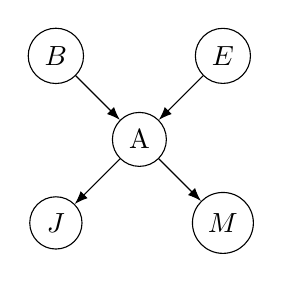
\begin{tikzpicture}[node distance=1.5cm]
      \node[draw,circle] (alarm) {A};
      \node[draw,circle,above left of=alarm] (burglary) {$B$};
      \node[draw,circle,above right of=alarm] (earthquake) {$E$};
      \node[draw,circle,below left of=alarm] (johnCalls) {$J$};
      \node[draw,circle,below right of=alarm] (maryCalls) {$M$};
      \draw[-Latex] (burglary) -- (alarm);
      \draw[-Latex] (earthquake) -- (alarm);
      \draw[-Latex] (alarm) -- (johnCalls);
      \draw[-Latex] (alarm) -- (maryCalls);
    \end{tikzpicture}
    \caption{a Bayesian network}
    \label{fig:bn}
  \end{subfigure}
  \begin{subfigure}{0.49\textwidth}
    \centering
    \begin{tikzpicture}[node distance=1.5cm]
      \node[draw,circle] (alarm) {A};
      \node[draw,circle,above left of=alarm] (burglary) {$B$};
      \node[draw,circle,above right of=alarm] (earthquake) {$E$};
      \node[draw,circle,below left of=alarm] (johnCalls) {$J$};
      \node[draw,circle,below right of=alarm] (maryCalls) {$M$};
      \draw[color=color1,ultra thick] (burglary) -- (earthquake);
      \draw[color=color1,ultra thick] (burglary) -- (alarm);
      \draw[color=color1,ultra thick] (earthquake) -- (alarm);
      \draw[color=color2,ultra thick] (alarm) -- (johnCalls);
      \draw[color=color3,ultra thick] (alarm) -- (maryCalls);
    \end{tikzpicture}
    \caption{a Markov network}\label{fig:mn}
  \end{subfigure}
  \caption{Two PGMs that describe the independence structure of \cref{example:bn}.}
\end{figure}

\begin{table}
  \centering
  \begin{tabular}[t]{lllr}
    \toprule
    $b$ & $e$ & $a$ & $\Pr(A = a \mid B = b, E = e)$ \\
    \midrule
    \false{} & \false{} & \false{} & 0.999 \\
    \false{} & \false{} & \true{} & 0.001 \\
    \false{} & \true{} & \false{} & 0.71 \\
    \false{} & \true{} & \true{} & 0.29 \\
    \true{} & \false{} & \false{} & 0.06 \\
    \true{} & \false{} & \true{} & 0.94 \\
    \true{} & \true{} & \false{} & 0.05 \\
    \true{} & \true{} & \true{} & 0.95 \\
    \bottomrule
  \end{tabular}
  \caption{An example CPT for $\Pr(A \mid B, E)$ from
    \cref{example:bn}.}\label{table:examplecpt}
\end{table}

The graph of a \emph{Bayesian network} for this example scenario is in
\cref{fig:bn}. This directed acyclic graph (DAG) tells us that the joint
probability distribution can be factored as
\begin{equation} \label{eq:factorisation}
  \Pr(B, E, A, J, M) = \Pr(B) \times \Pr(E) \times \Pr(A \mid B, E) \times \Pr(J \mid A) \times \Pr(M \mid A),
\end{equation}
i.e., the probability of each random variable is conditioned on its parents in
the graph. The factors in \cref{eq:factorisation} can be described using
\emph{conditional probability tables} (CPTs). CPTs assign a probability to each
combination of values that the random variable and its parents can take---see
\cref{table:examplecpt} for an example.

Alternatively, the same probability distribution can be represented as an
undirected PGM known as a \emph{Markov network} (or \emph{Markov random field}).
The graph of such a network for \cref{example:bn} is in \cref{fig:mn}. Here,
instead of CPTs, \emph{potentials} are the building blocks out of which a
probability distribution is constructed. A potential is a function from (some
subset of) random variables to non-negative real numbers. Potentials are
typically defined on the maximal cliques of the network. The edge sets of the
three maximal cliques in \cref{fig:mn} are highlighted in different colours.
Thus, the full probability distribution can be factored as
\[
\Pr(B, E, A, J, M) = \frac{1}{Z} \times \psi_1(B, E, A) \times \psi_2(A, J) \times \psi_3(A, M),
\]
where $\psi_1$, $\psi_2$, and $\psi_3$ are potentials, and $Z$ is a
normalisation constant known as the \emph{partition function}.

What if we wanted to generalise \cref{example:bn} to support any number of
neighbours, all of whom behave identically (i.e., have the same probabilities of
calling in all circumstances)? Both Bayesian and Markov networks have been
extended for such scenarios: \emph{relational Bayesian networks}
\citep{DBLP:conf/uai/Jaeger97} can compactly describe a probability distribution
over a relational structure, and \emph{Markov logic networks} (also known as
\emph{Markov logic}) \citep{DBLP:journals/ml/RichardsonD06} extend Markov
networks with support for first-order logic. The field of learning such
representations from data is known as \emph{statistical relational learning}
\citep{DBLP:series/synthesis/2016Raedt}. The next section describes relational
representations that are based on programming languages instead of graphical
models.

\subsection{Probabilistic Programming}\label{sec:probprogramming}

Augmenting a programming language with probabilities is another common way to
compactly represent probability distributions. Logic programming languages, in
particular, have been frequently used for this purpose. Examples of
probabilistic logic programming languages include the independent choice logic
\citep{DBLP:journals/ai/Poole97,DBLP:conf/ilp/Poole08}, PRISM
\citep{DBLP:conf/ijcai/SatoK97,DBLP:conf/ilp/SatoK08}, BLOG
\citep{DBLP:conf/ijcai/MilchMRSOK05}, NP-BLOG
\citep{DBLP:conf/uai/CarbonettoKFP05}, ProbLog \citep{DBLP:conf/ijcai/RaedtKT07}
and CP-logic \citep{DBLP:journals/tplp/VennekensDB09}. Functional and imperative
programming languages have also seen some use, examples of which include BUGS
\citep{gilks1994language}, IBAL \citep{DBLP:conf/ijcai/Pfeffer01}, Church
\citep{DBLP:conf/uai/GoodmanMRBT08}, and Stan \citep{stan}. More information on
probabilistic logic programming, probabilistic programming more generally, and
statistical relational artificial intelligence can be found in the work of
\citet{DBLP:conf/ilp/2008p}, \citet{DBLP:conf/icse/GordonHNR14}, and
\citet{DBLP:series/synthesis/2016Raedt}, respectively.

\begin{lstlisting}[caption=A ProbLog program that computes
  $\protect{\Pr(B \mid J, M)}$ for the scenario described in \cref{example:bn}.,
  label={lst:problog}]
  neighbour(john).
  neighbour(marry).

  0.001 :: burglary.
  0.002 :: earthquake.

  0.95  :: alarm :- burglary, earthquake.
  0.94  :: alarm :- burglary, \+ earthquake.
  0.29  :: alarm :- \+ burglary, earthquake.
  0.001 :: alarm :- \+ burglary, \+ earthquake.

  0.8   :: calls(X) :- alarm, neighbour(X).
  0.1   :: calls(X) :- \+ alarm, neighbour(X).

  evidence(calls(john)).
  evidence(calls(mary)).
  query(burglary).
\end{lstlisting}

\begin{lstlisting}[escapeinside={(*}{*)},caption=A BLOG program that computes
  $\protect{\Pr(B \mid J, M)}$ for the scenario described in \cref{example:bn}.,
  label={lst:blog}]
  type Neighbour;
  distinct Neighbour John, Mary;

  random Boolean Burglary   (*$\sim$*) BooleanDistrib(0.001);
  random Boolean Earthquake (*$\sim$*) BooleanDistrib(0.002);

  random Boolean Alarm (*$\sim$*) case[Burglary, Earthquake] in {
    [false, false] -> BooleanDistrib(0.001),
    [false, true]  -> BooleanDistrib(0.29),
    [true, false]  -> BooleanDistrib(0.94),
    [true, true]   -> BooleanDistrib(0.95)
  };

  random Boolean Calls(Neighbour n) (*$\sim$*)
    if Alarm then BooleanDistrib(0.8)
    else BooleanDistrib(0.1);

  obs Calls(John) = true;
  obs Calls(Mary) = true;
  query Burglary;
\end{lstlisting}

\Cref{lst:problog,lst:blog} contain two probabilistic programs that encode the
information in \cref{example:bn}. In preparation for \cref{chapter:randomlps},
let us examine the syntax and semantics of ProbLog a bit more closely. ProbLog
clauses are exactly like Prolog clauses (see \cref{sec:lp}) but with \verb+p ::+
prepended, for some probability \texttt{p}. Without \verb+::+, the probability
associated with the clause is implicitly equal to 1. ProbLog also has keywords
\texttt{evidence} and \texttt{query} that are used to define one or more
(potentially conditional) probabilities of interest. Reading off the
probabilities from \cref{lst:problog}, we can, e.g., compute the probability
that John calls as
\begin{align*}
  \Pr(j) &= \Pr(b)\Pr(e)\Pr(a \mid b, e)\Pr(j \mid a) \\
  &+ \Pr(b)\Pr(e)\Pr(\neg a \mid b, e)\Pr(j \mid \neg a) \\
  &+ \cdots \\
  &+ \Pr(\neg b)\Pr(\neg e)\Pr(\neg a \mid \neg b, \neg e)\Pr(j \mid \neg a) \\
  &= 0.001 \times 0.002 \times 0.95 \times 0.8 + \cdots \\
  &\approx 0.102.
\end{align*}
More formally, the probability of a query is the sum of the probabilities of the
models of the query (c.f. WMC).

\section{Knowledge Compilation and Representation}\label{sec:kc}
% Probabilistic SDDs \citep{DBLP:conf/kr/KisaBCD14} extend SDDs with probability
% labels on edges.

\emph{Knowledge compilation} is the process of transforming the initial
representation of some data (usually based on propositional logic) to a
representation that allows one to perform various operations and answer queries
of interest in time polynomial in the size of this new representation. Many such
representations have been proposed \citep{DBLP:journals/jair/DarwicheM02}.
Amongst them, those particularly relevant to WMC and probabilistic inference
are:
\begin{itemize}
  \item deterministic decomposable negation normal form (d-DNNF)
        \citep{DBLP:journals/jancl/Darwiche01},
  \item sentential decision diagrams (SDDs) \citep{DBLP:conf/ijcai/Darwiche11},
  \item (ordered) binary decision diagrams (BDDs)
        \citep{DBLP:journals/tc/Bryant86},
  \item and algebraic decision diagrams (ADDs)
        \citep{DBLP:journals/fmsd/BaharFGHMPS97}.
\end{itemize}
The first two items on this list are described in \cref{sec:nnf,sec:sdds},
respectively, and the last two are covered in a bit more detail in
\cref{sec:dds}. While knowledge compilation is a process (which is performed by
algorithms), here our focus is on the representations themselves.

\subsection{NNF and d-DNNF}\label{sec:nnf}

\begin{definition}
  A propositional formula $\phi$ is in \emph{negation normal form} (NNF) if
  \begin{itemize}
    \item the only operators in $\phi$ are $\neg$, $\lor$, and $\land$,
    \item and $\neg$ is only applied to directly to variables.
  \end{itemize}
\end{definition}

\begin{example}
  Formula $\neg(C \Rightarrow (\neg A \land B))$ can be transformed into NNF as
  follows:
  \[
  \neg(C \Rightarrow (\neg A \land B)) \equiv \neg(\neg C \lor (\neg A \land B)) \equiv C \land (A \lor \neg B)
  \]
  using the definition of $\Rightarrow$ and De Morgan's laws.
\end{example}

\begin{definition}
  The d-DNNF adds decomposability and determinism to the NNF\@.
  \emph{Decomposability} requires that, for every conjunction
  $\bigwedge_{i=1}^n \phi_i$, conjuncts $\phi_i$ and $\phi_j$ have no variables
  in common for all $i \ne j$
  \citep{DBLP:conf/ijcai/Darwiche99,DBLP:journals/jacm/Darwiche01}.
  \emph{Determinism} requires that, for every disjunction
  $\bigvee_{i=1}^n \phi_i$, disjuncts $\phi_i$ and $\phi_j$ contradict each
  other (i.e., $\phi_i \land \phi_j \equiv \bot$) for all $i \ne j$
  \citep{DBLP:journals/jancl/Darwiche01}.
\end{definition}

\begin{example}
  Formula $(A \lor \neg B) \land (A \lor C)$ is neither decomposable nor
  deterministic. It is not decomposable because
  $\{\, A, B \,\} \cap \{\, A, C \,\} = \{\, A \,\} \ne \emptyset$. It is not
  deterministic because, e.g., $A \land \neg B \not\equiv \bot$.
\end{example}

\begin{example}\label{example:ddnnf1}
  Formula $C \land (A \lor \neg B)$ is decomposable but not deterministic. It is
  decomposable because $\{\, C \,\} \cap \{\, A, B \,\} = \emptyset$. It is not
  deterministic because $A \land \neg B \not\equiv \bot$.
\end{example}

\begin{example}
  Formula $B \land C \land [\neg B \lor (A \land B)]$ is deterministic but not
  decomposable. It is deterministic because
  $\neg B \land A \land B \equiv \bot$. It is not decomposable because
  $\{\, B \,\} \cap \{\, A, B \,\} = \{\, B \,\} \ne \emptyset$.
\end{example}

\begin{example}\label{example:ddnnf2}
  Formula $C \land [\neg B \lor (A \land B)]$ is decomposable and deterministic.
  It is decomposable because $\{\, C \,\} \cap \{\, A, B \,\} = \emptyset$, and
  $\{\, A \,\} \cap \{\, B \,\} = \emptyset$. It is deterministic because
  $\neg B \land A \land B \equiv \bot$.
\end{example}

\begin{figure}
  \centering
  \begin{subfigure}{0.32\textwidth}
    \centering
    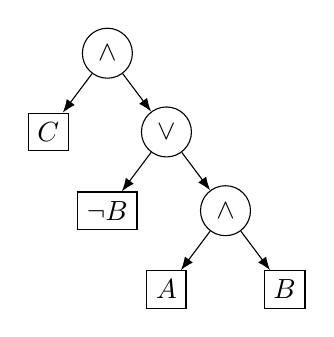
\begin{tikzpicture}[level distance=1cm,edge from
      parent/.style={draw,-Latex}] % C \land [\neg B \lor (A \land B)]
      \node[draw,circle] {$\land$}
      child {node[draw,rectangle] {$C$}}
      child {node[draw,circle] {$\lor$}
        child {node[draw,rectangle] {$\neg B$}}
        child {node[draw,circle] {$\land$}
          child {node[draw,rectangle] {$A$}}
          child {node[draw,rectangle] {$B$}}
        }
      };
    \end{tikzpicture}
    \caption{d-DNNF}\label{fig:ddnnf}
  \end{subfigure}
  \begin{subfigure}{0.32\textwidth}
    \centering
    \begin{tikzpicture}[level distance=1cm,edge from
      parent/.style={draw,-Latex}]
      \tikzset{
        mysplit/.style={
          draw,
          rectangle,
          rectangle split,
          rectangle split horizontal,
          rectangle split parts=2
        }
      }
      \node[draw,circle] {$1$}
      child {node[mysplit] (bullet) {
          \nodepart{one} $\neg A$
          \nodepart{two}
        }
        child {node[draw,circle] (3) {$3$} edge from parent[draw=none]
          child {node[mysplit] {
              \nodepart{one} $\neg B$
              \nodepart{two} $C$
            }
          }
          child {node[mysplit] {
              \nodepart{one} $B$
              \nodepart{two} $\bot$
            }
          }
        }
      }
      child {node[mysplit] {
          \nodepart{one} $A$
          \nodepart{two} $C$
        }};
      \draw[*-Latex] let \p1 = (bullet.two), \p2 = (bullet.center) in ({\x1 + 2.5},{\y2 + 2}) -- (3);
    \end{tikzpicture}
    \caption{SDD}\label{fig:sdd}
  \end{subfigure}
  \begin{subfigure}{0.32\textwidth}
    \centering
    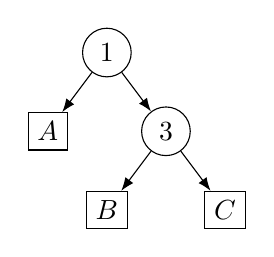
\begin{tikzpicture}[level distance=1cm,edge from
      parent/.style={draw,-Latex}]
      \node[draw,circle] {$1$}
      child {node[draw,rectangle] {$A$}}
      child {node[draw,circle] {$3$}
        child {node[draw,rectangle] {$B$}}
        child {node[draw,rectangle] {$C$}}
      };
    \end{tikzpicture}
    \caption{vtree}\label{fig:vtree}
  \end{subfigure}
  \caption{A d-DNNF and an SDD representation of $C \land (A \lor \neg B)$,
    together with the corresponding vtree. The numbers 1 and 3 come from the
    in-order traversal of the vtree and visually connect subtrees of both the
    SDD and the vtree.}\label{fig:kc}
\end{figure}

Note that the formulas in \cref{example:ddnnf1,example:ddnnf2} are equivalent,
and the latter is also pictured in \cref{fig:ddnnf}.

\subsection{SDDs}\label{sec:sdds}

To define SDDs, we first need to define vtrees.

\begin{definition}[\citep{DBLP:conf/aaai/PipatsrisawatD08}]
  A \emph{vtree} for a set of variables $X$ is a full binary tree $T$ with a
  bijection between $X$ and the leaves of $T$.
\end{definition}

Let $\langle\cdot\rangle$ denote the function that maps an SDD to the
propositional formula that it represents.

\begin{definition}[\citep{DBLP:conf/ijcai/Darwiche11}]
  Let $V$ be a vtree for a set of variables $X$. Then $S$ is an \emph{SDD} that
  respects $V$ if one of the following is true:
  \begin{itemize}
    \item $S = \bot$ ($\langle \bot \rangle \coloneqq \bot$);
    \item $S = \top$ ($\langle \top \rangle \coloneqq \top$);
    \item $S = x$, or $S = \neg x$, where $x \in X$ is the variable bijectively
          associated with the \emph{only} node of $V$
          ($\langle x \rangle \coloneqq x$, and
          $\langle \neg x \rangle \coloneqq \neg x$);
    \item $S = \{\, (p_i, s_i) \mid i = 1, \dots, n \,\}$ for some $n \ge 1$,
          where \emph{primes} ${\{\,p_i\,\}}_{i=1}^n$ and \emph{subs}
          ${\{\,s_i\,\}}_{i=1}^n$ are SDDs such that:
    \begin{itemize}
      \item $V$ has more than one node,
      \item each $p_i$ respects the left subtree of $V$,
      \item each $s_i$ respects the right subtree fo $V$.
      \item the primes form a \emph{partition}, i.e.:
      \begin{itemize}
        \item $\langle p_i \rangle \not\equiv \bot$ for all $i = 1, \dots, n$
              (i.e., the primes are \emph{consistent}),
        \item $\langle p_i \rangle \land \langle p_j \rangle \equiv \bot$ for
              all $i \ne j$ (i.e., the primes are \emph{mutually exclusive}),
        \item and $\bigvee_{i=1}^n \langle p_i \rangle \equiv \top$
      \end{itemize}
    \end{itemize}
    (then $\langle S \rangle \coloneqq \bigvee_{i=1}^n \langle p_i \rangle \land \langle s_i \rangle$).
  \end{itemize}
\end{definition}

\begin{example}
  Let $S = \{\, (A, C), (\neg A, \{\, (\neg B, C), (B, \bot) \,\}) \,\}$. Then
  $S$ (as pictured in \cref{fig:sdd}) is an SDD representation of
  $C \land (A \lor \neg B)$ that respects the vtree in \cref{fig:vtree}. Indeed,
  \begin{align*}
    \langle S \rangle &= (A \land C) \lor (\neg A \land [(\neg B \land C) \lor (B \land \bot)]) \\
    &\equiv (A \land C) \lor (\neg A \land \neg B \land C) \\
    &\equiv C \land (A \lor [\neg A \land \neg B]) \\
    &\equiv C \land ([A \lor \neg A] \land [A \lor \neg B]) \\
    &\equiv C \land (\top \land [A \lor \neg B]) \\
    &\equiv C \land (A \lor \neg B).
  \end{align*}
\end{example}

\subsection{Other Decision Diagrams}\label{sec:dds}

NNF and d-DNNF are \emph{normal forms} of propositional formulas. This means
that---even though they can be represented diagrammatically as trees or
circuits---a formula in (d-D)NNF (just like in CNF) is still a formula. The same
applies to SDDs: while we defined them as nested sets and tuples,
$\langle S \rangle$ of an SDD $S$ is just a propositional formula with a certain
structure. In contrast, the two representations we describe here---BDDs and
ADDs---are defined as DAGs rather than normal forms.

Both BDDs and ADDs represent functions. BDDs represent \emph{Boolean functions},
i.e., maps of the form ${\{\, 0, 1 \,\}}^n \to \{\, 0, 1 \,\}$ for some
$n \ge 0$, where $\{\, 0, 1 \,\}$ can be replaced by any other two-element set.
A propositional formula is simply a particular representation of a Boolean
function. ADDs, on the other hand, represent \emph{pseudo-Boolean functions},
i.e., maps of the form ${\{ 0, 1 \}}^n \to \mathbb{R}$. Equivalently, we can
write $2^X$ for ${\{\, 0, 1 \,\}}^n$, where $X$ is any $n$-element set, and
$2^X$ denotes its powerset. The elements of $X$ are then called
\emph{variables}. With this characterisation, pseudo-Boolean functions are also
known as \emph{set functions}.

Pseudo-Boolean functions, most commonly represented as ADDs (although a
tensor-based approach has also been suggested
\citep{DBLP:journals/corr/abs-1908-04381,DBLP:conf/cp/DudekPV20}), have seen
extensive use in value iteration for Markov decision processes
\citep{DBLP:conf/uai/HoeySHB99}, both exact and approximate Bayesian network
inference \citep{DBLP:conf/ijcai/ChaviraD07,DBLP:conf/uai/GogateD11}, and
sum-product network to Bayesian network conversion
\citep{DBLP:conf/icml/ZhaoMP15}. ADDs have been extended to compactly represent
additive and multiplicative patterns in the image of the function
\citep{DBLP:conf/ijcai/SannerM05} and to support first-order logic
\citep{DBLP:journals/ai/SannerB09} and continuous variables
\citep{DBLP:conf/uai/SannerDB11}. This last extension was also applied to
weighted model integration, i.e., the WMC extension for continuous variables
\citep{DBLP:conf/ijcai/BellePB15,DBLP:conf/ijcai/KolbMSBK18}.

Informally, both BDDs and ADDs are like decision trees (whose leaves correspond
to elements of the image of the function that is being represented) but
compressed into a DAG\@. Below we define ADDs---the definition of BDDs simply
requires replacing $\mathbb{R}$ with $\{\, 0, 1 \,\}$. Our definition is
partially based on the original definition by
\citet{DBLP:journals/fmsd/BaharFGHMPS97} as well as recent work by
\citet{DBLP:conf/cp/DudekPV20} but states some details more explicitly. The
definition can also be generalised to use any set instead of $\mathbb{R}$ and to
represent several functions instead of just one.

\paragraph*{Notation.}
Let $G$ be a directed graph. Then $\mathcal{V}(G)$ denotes the set of nodes of
$G$, $\mathcal{E}(G)$ denotes the set of edges of $G$, and $\mathcal{L}(G)$
denotes the set of sinks of $G$.

\begin{definition}\label{def:add}
  Given a set of variables $X$ and a variable ordering represented as an
  injection $\sigma\colon X \to \mathbb{N}^+$, an \emph{ADD} is a tuple
  $(G, r, \rho, \chi, \epsilon)$ where:
  \begin{itemize}
    \item $G$ is a rooted DAG with root $r \in \mathcal{V}(G)$ (i.e., there is a
          directed path from $r$ to any other node),
    \item $\rho\colon \mathcal{L}(G) \to \mathbb{R}$ labels sinks with real
          numbers,
    \item $\chi\colon \mathcal{V}(G) \setminus \mathcal{L}(G) \to X$ labels
          other nodes with variable names,
    \item and $\epsilon\colon \mathcal{E}(G) \to \{\,0, 1\,\}$ labels edges.
  \end{itemize}
  Moreover, the following properties must be satisfied.
  \begin{itemize}
    \item Every node has outdegree either zero or two. In the latter case, the
          two outgoing edges $e, f \in \mathcal{E}(G)$ are such that
          $\epsilon(e) \ne \epsilon(f)$. If $e = (v, u)$, and $f = (v, w)$ for
          some $u, v, w \in \mathcal{V}(G)$ are such that $\epsilon(e) = 1$, and
          $\epsilon(f) = 0$, then $u$ is the \emph{positive successor} of $v$,
          and $w$ is the \emph{negative successor} of $v$.
    \item For every directed path with node sequence $v_1, v_2, \dots, v_n$ such
          that $v_i \not\in \mathcal{L}(G)$ for all $i$, we have that
          $\sigma(\chi(v_i)) < \sigma(\chi(v_{i+1}))$ for all
          $i = 1, 2, \dots, n - 1$.
  \end{itemize}
  We say that an ADD \emph{has} variable $x \in X$ if there is a node
  $v \in \mathcal{V}(G) \setminus \mathcal{L}(G)$ such that $\chi(v) = x$.
\end{definition}

To view an ADD as a pseudo-Boolean function, given an interpretation
$\iota\colon X \to \{\, \true{}, \false{} \,\}$, start at the root and follow
the outgoing edges until you reach a sink. If at node
$v \in \mathcal{V}(G) \setminus \mathcal{L}(G)$ we have that
$\iota(\chi(v)) = \true{}$, then follow the outgoing edge $e$ with
$\epsilon(e) = 1$, otherwise follow the outgoing edge $f$ with
$\epsilon(f) = 0$. Once you reach a sink $l \in \mathcal{L}(G)$, then $\rho(l)$
is the value of the represented function at $\iota$ (where $\iota$ is
interpreted as a subset of $X$).

\begin{figure}
  \centering
  \begin{subfigure}{0.49\textwidth}
    \centering
    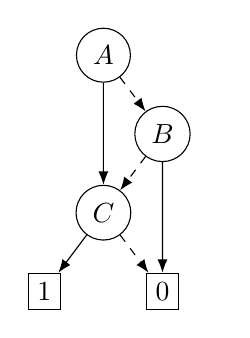
\begin{tikzpicture}[level distance=1cm,edge from
      parent/.style={draw,-Latex}]
      \node[draw,circle] (A) {$A$}
      child {edge from parent[draw=none]}
      child {node[draw,circle] (B) {$B$} edge from parent[dashed]
        child {node[draw,circle,solid] (C) {$C$} edge from parent[dashed]
          child {node[draw,rectangle,solid] {$1$} edge from parent[solid]}
          child {node[draw,rectangle,solid] (0) {$0$}}
        }
        child {edge from parent[draw=none]}
      };
      \draw[-Latex] (A) -- (C);
      \draw[-Latex] (B) -- (0);
    \end{tikzpicture}
    \caption{BDD}\label{fig:bdd}
  \end{subfigure}
  \begin{subfigure}{0.49\textwidth}
    \centering
    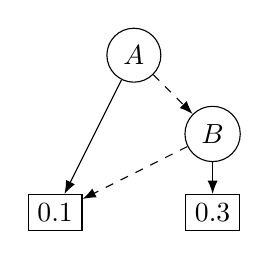
\begin{tikzpicture}
      \node[circle,draw] (x) at (0, 0) {$A$};
      \node[circle,draw] (y) at (1, -1) {$B$};
      \node[draw] (a) at (-1, -2) {0.1};
      \node[draw] (b) at (1, -2) {0.3};
      \draw[dashed,-Latex] (x) -- (y);
      \draw[-Latex] (x) -- (a);
      \draw[dashed,-Latex] (y) -- (a);
      \draw[-Latex] (y) -- (b);
    \end{tikzpicture}
    \caption{ADD}\label{fig:add}
  \end{subfigure} % could redraw the second diagram to be more like the others
  \caption{Example BDD (for the formula $C \land (A \lor \neg B)$) and ADD (for
    the function $f$ in \cref{example:add}). An edge $e$ is dashed if
    $\epsilon(e) = 0$ and solid otherwise, where $\epsilon$ is as in
    \cref{def:add}.}
\end{figure}

\begin{example}\label{example:add}
  Let $f\colon 2^{\{\,x, y\,\}} \to \mathbb{R}$ be a pseudo-Boolean function
  defined as $f(\emptyset) = f(\{\,x\,\}) = f(\{\,x, y\,\}) = 0.1$, and
  $f(\{\,y\,\}) = 0.3$ and $\sigma\colon \{\,x, y\,\} \to \mathbb{N}^+$ be the
  variable ordering function defined as $\sigma(x) = 1$, and $\sigma(y) = 2$.
  Then the \emph{canonical} ADD for $f$ under $\sigma$ is pictured in
  \cref{fig:add}\footnote{Also see \cref{fig:bdd} for a BDD equivalent to the
    d-DNNF and the SDD in \cref{fig:kc}.} and can be formally defined as
  $(G, a, \rho, \chi, \epsilon)$, where:
  \begin{itemize}
    \item $\mathcal{V}(G) = \{\,a, b, c, d\,\}$,
    \item $\mathcal{E}(G) = \{\,(a, b), (a, c), (b, c), (b, d)\,\}$,
    \item $\rho(c) = 0.1$, $\rho(d) = 0.3$,
    \item $\chi(a) = A$, $\chi(b) = B$,
    \item $\epsilon((a, c)) = \epsilon((b, d)) = 1$, and
          $\epsilon((a, b)) = \epsilon((b, c)) = 0$.
  \end{itemize}
\end{example}

We end our discussion of BDDs and ADDs by describing some of their properties as
well as operations on them.

\begin{fact}[\citet{DBLP:journals/fmsd/BaharFGHMPS97}]
  Let $X$ be a set of variables and $\sigma\colon X \to \mathbb{N}^+$ be an
  ordering function. For any subset of variables $Y \subseteq X$ and
  pseudo-Boolean function $f\colon 2^Y \to \mathbb{R}$, there is a unique (up to
  isomorphism) \emph{canonical} ADD for $f$. Any ADD for $f$ can be
  \emph{reduced} to its canonical form in time linear in the number of nodes.
\end{fact}

\begin{fact}\label{lemma:add_size}
  The canonical ADD for a pseudo-Boolean function $2^X \to \mathbb{R}$ has at
  most $2^{|X|+1}$ nodes. This upper bound is achieved when the function is
  injective.
\end{fact}

\begin{table}
  \centering
  \begin{tabular}{lll}
    \toprule
    Operation & Definition & Complexity \\
    \midrule
    reduce $f$ & & $\mathcal{O}(n)$ \\
    $r+f$, $rf$ & $r+f\colon 2^X \to \mathbb{R}$, $(r+f)(Z) \coloneqq r+f(Z)$ & $\mathcal{O}(n)$ \\
    $f+g$, $fg$ & $f+g\colon 2^{X \cup Y} \to \mathbb{R}$, $(f+g)(Z) \coloneqq f(Z)+g(Z)$ & $\mathcal{O}(mn)$ \\
    $f|_{x=0}$ & $f|_{x=0}\colon 2^{X \setminus \{\,x\,\}} \to \mathbb{R}$, $f|_{x=0}(Z) \coloneqq f(Z)$ & $\mathcal{O}(n)$ \\
    $f|_{x=1}$ & $f|_{x=1}\colon 2^X \to \mathbb{R}$, $f|_{x=1}(Z) \coloneqq f(Z \cup \{\,x\,\})$ & $\mathcal{O}(n)$ \\
    $\exists_xf$ & $\exists_xf\colon 2^{X \setminus \{\,x\,\}} \to \mathbb{R}$, $\exists_xf(Z) \coloneqq f|_{x=0}(Z) + f|_{x=1}(Z)$ & $\mathcal{O}(n^2)$ \\
    \bottomrule
  \end{tabular}
  \caption{Operations on ADDs, their definitions, and the time complexity of the
    best-known algorithm for performing each operation. Let
    $f\colon 2^X \to \mathbb{R}$ and $g\colon 2^Y \to \mathbb{R}$ be
    pseudo-Boolean functions represented by ADDs with $n$ and $m$ nodes
    respectively, and let $r \in \mathbb{R}$, and
    $x \in X$.}\label{tbl:complexity}
\end{table}

The operations pertinent to our needs are listed in \cref{tbl:complexity}:
reduction of an ADD to its canonical form, addition/multiplication as well as
scalar addition/multiplication, two types of \emph{restrictions}, and
\emph{projection}. For a more detailed description, we refer the reader to
previous work \citep{DBLP:journals/fmsd/BaharFGHMPS97,DBLP:conf/aaai/DudekPV20}.
The linear reduction algorithm is by \citet{somenzi1998cudd}, the algorithms for
most other operations are by \citet{DBLP:journals/tc/Bryant86}, and the
complexity of projection comes as a corollary of the complexities of all other
operations.

When referring to ADDs and their use in algorithms, we make a few simplifying
assumptions. First, we assume that projection has the lowest precedence and
extend the definition to allow for sets of variables. For any
$W = {\{\,w_i\,\}}_{i=1}^k \subseteq X$, let
$\exists_W f\colon 2^{X \setminus W} \to \mathbb{R}$ be defined as
$\exists_{W}f(Z) \coloneqq \exists_{w_1}\exists_{w_2}\cdots\exists_{w_k}f(Z)$
for all $Z \subseteq X \setminus W$, where the order of $w_i$'s is immaterial.
Second, we assume that after every operation on ADDs, the resulting ADD is
reduced to its canonical form and write `the ADD for function $f$' to mean `the
\emph{canonical} ADD for $f$'. Third, while ADDs and the functions they
represent could change throughout the execution of an algorithm, we consider the
set of all relevant variables $X$ and the ordering function
$\sigma\colon X \to \mathbb{N}^+$ to be fixed.

% could add an example of operations

% BDDs are a strict subset of SDDs that are a strict subset of d-DNNF \citep{DBLP:conf/ijcai/Darwiche11}.

%% \begin{lemma} \label{lemma:clause_time}
%%   Let $\phi$ be a conjunction/disjunction of $n$ literals. Then the ADD for
%%   $[\phi]^p_q$ (for any $p, q \in \mathbb{R}$ such that $p \ne q$) can be
%%   constructed in $\mathcal{O}(2^n)$ time.
%% \end{lemma}
%% \begin{proof}
%%   The ADD for $[\phi]_0^1$ can be constructed with a sequence of $n-1$ binary
%%   operations, with one of the two operands always the ADD representation of a
%%   literal. The number of variables in the other operand then follows the
%%   sequence $1, 2, 3, \dots, n-1$. By \cref{lemma:add_size}, the numbers of nodes
%%   in the ADDs for these operands is then $2^2, 2^3,
%%   \dots, 2^n$. Since one of the operands is of constant size,
%%   the overall time complexity of all binary operations is then
%%   $\sum_{i=2}^n \mathcal{O}(2^i) = \mathcal{O}(2^n)$. Finally, note that
%%   $[\phi]_q^p = (p-q)[\phi]_0^1 + q$. As scalar operations can be performed in
%%   linear time, the overall complexity remains $\mathcal{O}(2^n)$.
%% \end{proof}

\section{Applications of WMC}\label{sec:applications}

% could mention the StarAI book

WMC is heavily used in machine learning, where recent applications of WMC
include explainability \citep{DBLP:conf/aaai/BroeckLSS21} and computing the loss
function of a neural-symbolic system
\citep{DBLP:conf/aaai/TsamouraHM21,DBLP:conf/icml/XuZFLB18}. The most
well-researched application of WMC, however, is inference for PGMs such as
Bayesian networks
\citep{DBLP:conf/ecai/BartKLM16,DBLP:conf/ijcai/ChaviraD05,DBLP:conf/sat/ChaviraD06,DBLP:conf/kr/Darwiche02,DBLP:conf/aaai/SangBK05}.
Originally, this approach was motivated by \emph{context-specific independence},
i.e., the independence of random variables that is created by conditioning the
probability distribution \citep{DBLP:conf/uai/BoutilierFGK96}. Deconstructing a
graphical model to a propositional formula makes such independencies easier to
exploit \citep{DBLP:conf/kr/Darwiche02}. Moreover, WMC is used for inference in
probabilistic programming languages such as ProbLog
\citep{DBLP:journals/tplp/FierensBRSGTJR15,DBLP:conf/aaai/VlasselaerKDMR16} and
Dice \citep{DBLP:journals/pacmpl/HoltzenBM20}.

Indeed, WMC and WFOMC play an important role in inference for statistical
relational models such as ProbLog and Markov logic
\citep{DBLP:series/synthesis/2016Raedt,DBLP:conf/nips/Broeck11}. Such models are
often used in natural language processing for tasks such as
knowledge/information extraction
\citep{bunescu2007statistical,DBLP:conf/naacl/PoonV10}. In natural language
processing, statistical relational models have been used to annotate articles
\citep{DBLP:conf/emnlp/VerbekeAMFDR12}, learn facts about the world from reading
websites \citep{DBLP:conf/aaai/CarlsonBKSHM10}, and solve simple probability
problems described in a natural language \citep{DBLP:conf/ijcai/DriesKDBR17}.
Similarly, they have been applied to stream mining
\citep{DBLP:conf/icdm/ChandraSKTA14}, predicting criminal activity
\citep{DBLP:conf/sdm/DelaneyFCWJ10}, and predicting how soon a component or a
machine will have to be replaced \citep{vlasselaer2012statistical}. In robotics,
statistical relational models have been used to learn object affordances
\citep{DBLP:conf/ilp/MoldovanORMS11,DBLP:conf/icra/MoldovanMOSR12,DBLP:conf/iros/MoldovanR14}
and as an expressive knowledge representation system for robot control
\citep{DBLP:conf/icra/JainMB09}. Finally, applications in bioinformatics include
the analysis of breast cancer
\citep{DBLP:conf/ilp/Corte-RealD017,DBLP:conf/pkdd/NassifKBPSC13}, genetic
\citep{DBLP:journals/jcb/SakhanenkoG12}, and molecular profiling
\citep{de2013phenetic} data.

\todo[inline]{ Is it worth adding a small comment on how you expect the
  contributions of this thesis to connect to some of this work Something along
  the lines of: although it is hard to anticipate how the contributions of this
  work might affect all of these applications, we immediately see that
  improvements in terms of inference and encoding can affect the modelling and
  solving of probabilistic frameworks such as programs and networks. }
 % 11-45 pages (27 on average)
\chapter{WMC Without Parameter Variables}\label{chapter:wmc2}

\section{Introduction}

Recall that in \cref{chapter:wmc1} we examined WMC from a measure-theoretic
perspective and found that---due to the rigidity of the standard
formulation---WMC encodings usually contain many superfluous variables. This
observation inspired an encoding for Bayesian networks that alleviates the
issue. In this chapter, we continue to tackle the subject of superfluous
parameter variables but take the solution a few steps further.

If WMC is not the right format for probabilistic inference and other
sum-of-products computations, what could be a better alternative? As many WMC
inference algorithms \citep{DBLP:conf/ecai/Darwiche04,DBLP:conf/ijcai/OztokD15}
work by compilation to tractable representations such as arithmetic circuits,
deterministic, decomposable negation normal form
\citep{DBLP:journals/jancl/Darwiche01}, and sentential decision diagrams (SDDs)
\citep{DBLP:conf/ijcai/Darwiche11}, perhaps parameter variables could be avoided
via direct compilation to a more convenient representation. Direct compilation
of Bayesian networks to SDDs has been investigated
\citep{DBLP:conf/ecsqaru/ChoiKD13}. However, SDDs only support weights on
literals, and so are not expressive enough to avoid the issue.
\Citet{DBLP:conf/uai/GogateD10} propose a format based on weighted clauses and
probabilistic semantics inspired by Markov networks. However, with a new
representation comes the need to invent new encodings and inference algorithms.
Moreover, to the best of our knowledge, neither approach
\citep{DBLP:conf/ecsqaru/ChoiKD13,DBLP:conf/uai/GogateD10} has a publicly
available implementation.

In this work, we introduce a new computational problem called
\emph{pseudo-Boolean projection} (PBP)---a generalisation of the conditional
weights approach proposed in \cref{chapter:wmc1}. Recent WMC algorithms based on
pseudo-Boolean function manipulation---namely, \textsc{ADDMC}
\citep{DBLP:conf/aaai/DudekPV20} and \textsc{DPMC}
\citep{DBLP:conf/cp/DudekPV20}---can easily be adapted to the new format. In
contrast to our previous work, instead of inventing new encodings, we show how
every WMC problem instance can be transformed to PBP and identify conditions
under which this transformation can remove parameter variables. Four out of the
five known WMC encodings for Bayesian networks
\citep{DBLP:conf/ecai/BartKLM16,DBLP:conf/ijcai/ChaviraD05,DBLP:conf/sat/ChaviraD06,DBLP:conf/kr/Darwiche02,DBLP:conf/aaai/SangBK05}
can indeed be simplified in this manner. We are able to eliminate
\SI{43}{\percent} of variables on average and up to \SI{99}{\percent} on some
instances. This transformation enables two encodings that were previously
incompatible with most WMC algorithms (due to using a different formulation of
WMC \citep{DBLP:conf/ijcai/ChaviraD05,DBLP:conf/sat/ChaviraD06}) to be run with
\textsc{ADDMC} and \textsc{DPMC} and results in a significant performance boost
for one other encoding, making it about three times faster than the state of the
art. Finally, our theoretical contributions result in a convenient algebraic way
of reasoning about two-valued pseudo-Boolean functions and position WMC
encodings on common ground, identifying their key properties and assumptions.

% Specifically, direct compilation
% from Bayesian networks to SDDs \citep{DBLP:conf/ecsqaru/ChoiKD13} and from
% structured Bayesian networks (i.e., a generalisation of Bayesian networks) to
% probabilistic SDDs \citep{shen2020modeling} have been considered.

% * SDD compilation still has parameter variables
% 1) However, no conversion algorithms from either WMC or probabilistic models
% are provided.
% Since we present a WMC to PBP algorithm, we don't need to invent new
% encodings for each problem and we can benefit from all the good ideas that
% went into designing WMC encodings
% 3) Instead of combining techniques from older WMC algorithms like they did, we
% use a much more recent WMC solver that is shown to...
% 3) We benefit from a decade of research in WMC inference and, specifically, 
% 4) We are not restricted to clauses and probabilistic semantics
% 5) We identify conditions and describe an algorithm for transforming any WMC
% instance into PBP

\section{Redefining WMC}

Since the goal of this chapter is to generalise WMC in a way that eliminates the
redundant parameter variables, in this section we redefine WMC in a way that
explicitly partitions all variables into parameter and indicator variables. We
also formalise a variant of WMC that has been implicitly used by
\citet{DBLP:conf/ijcai/ChaviraD05,DBLP:conf/sat/ChaviraD06}.

In this chapter, we denote interpretations (and models) of a propositional
formula as subsets of the set of variables. These variables are implicitly
mapped to \texttt{true} whereas all other variables are mapped to
\texttt{false}. The \emph{cardinality} of a model is then the cardinality of
this set.

\begin{example}
  Let $\phi = (\neg a \lor b) \land a$ be a propositional formula over variables
  $a$ and $b$. Then $\{\, a, b \,\}$ (i.e.,
  $\{\, a \mapsto \texttt{true}, b \mapsto \texttt{true} \,\}$) is a model of
  $\phi$ (written $\{\, a, b \,\} \models \phi$), and it has cardinality two.
\end{example}

\begin{definition}[WMC]\label{def:wmc}
  A \emph{WMC instance} is a tuple $(\phi, X_I, X_P, w)$, where $X_I$ is the set
  of \emph{indicator variables}, $X_P$ is the set of \emph{parameter variables}
  (with $X_I \cap X_P = \emptyset$), $\phi$ is a propositional formula in CNF
  over $X_I \cup X_P$, and
  $w\colon X_I \cup X_P \cup \{\, \neg x \mid x \in X_I \cup X_P \,\} \to \mathbb{R}$
  is a \emph{weight function} such that $w(x) = w(\neg x) = 1$ for all
  $x \in X_I$. The \emph{answer} of the instance is
  $\sum_{Y \models \phi} \prod_{Y \models l} w(l)$.
\end{definition}

In practice, we identify this partition of variables in one of two ways. If an
encoding is generated by \textsc{Ace}\footnote{\textsc{Ace}
  \citep{DBLP:journals/ai/ChaviraD08} implements most of the Bayesian network
  encodings and can also be used for compilation (and thus inference). It is
  available at \url{http://reasoning.cs.ucla.edu/ace/}.}, then variable types
are explicitly identified in a file generated alongside the encoding. Otherwise,
we take $X_I$ to be the set of all variables $x$ such that
$w(x) = w(\neg x) = 1$. Next, we formally define another variant of WMC\@.

\begin{definition}
  Let $\phi$ be a formula over a set of variables $X$. Then $Y \subseteq X$ is a
  \emph{minimum-cardinality model} of $\phi$ if $Y \models \phi$ and $|Y| \le
  |Z|$ for all $Z \models \phi$.
\end{definition}

\begin{definition}[Minimum-cardinality WMC]\label{def:mcwmc}
  A \emph{minimum-cardinality WMC} instance consists of the same tuple as a WMC
  instance, but its \emph{answer} is defined to be
  \[
  \sum_{Y \models \phi\text{,}|Y| = k} \prod_{Y \models l} w(l)
  \]
  (where $k = \min_{Y \models \phi} |Y|$) if $\phi$ is satisfiable, and zero otherwise.
\end{definition}

\begin{example}\label{example:1}
  Let
  $\phi = (x \lor y) \land (\neg x \lor \neg y) \land (\neg x \lor p) \land (\neg y \lor q) \land x$,
  $X_I = \{\, x, y \,\}$, $X_P = \{\, p, q \,\}$, $w(p) = 0.2$, $w(q) = 0.8$,
  and $w(\neg p) = w(\neg q) = 1$. Then $\phi$ has two models: $\{\, x, p \,\}$
  and $\{\, x, p, q \,\}$ with weights $0.2$ and $0.2 \times 0.8 = 0.16$,
  respectively. The WMC answer is then $0.2 + 0.16 = 0.36$, and the
  minimum-cardinality WMC answer is $0.2$.
\end{example}

\section{Bayesian Network Encodings}\label{sec:encodings}

Recall that a \emph{Bayesian network} is a directed acyclic graph with random
variables as nodes and edges as conditional dependencies. As is common in
related literature \citep{DBLP:conf/kr/Darwiche02,DBLP:conf/aaai/SangBK05}, we
assume that each variable has a finite number of values. We call a Bayesian
network \emph{binary} if every variable has two values.

WMC is a well-established technique for Bayesian network inference, particularly
effective on networks where most variables have only a few possible values
\citep{DBLP:conf/kr/Darwiche02}. Many ways of encoding a Bayesian network into a
WMC instance have been proposed. \Citet{DBLP:conf/kr/Darwiche02} was the first
to suggest the \texttt{d02} encoding that, in many ways, remains the foundation
behind most other encodings. He also introduced the distinction between
\emph{indicator} and \emph{parameter variables}; the former represent
variable-value pairs in the Bayesian network, while the latter are associated
with probabilities in the conditional probability tables (CPTs). The encoding
\texttt{sbk05} \citep{DBLP:conf/aaai/SangBK05} is the only encoding that
deviates from this arrangement: for each variable in the Bayesian network, one
indicator variable acts simultaneously as a parameter variable.
\Citet{DBLP:conf/ijcai/ChaviraD05} propose \texttt{cd05} where they shift from
WMC to minimum-cardinality WMC because that allows the encoding to have fewer
variables and clauses. In particular, they propose a way to use the same
parameter variable to represent all probabilities in a CPT that are equal and
keep only clauses that `imply' parameter variables (i.e., omit clauses where a
parameter variable implies indicator variables).\footnote{\Cref{example:2}
  demonstrates what we mean by implication clauses.} In their next encoding,
\texttt{cd06}, \citet{DBLP:conf/sat/ChaviraD06} optimise the aforementioned
implication clauses, choosing the smallest sufficient selection of indicator
variables. A decade later, \citet{DBLP:conf/ecai/BartKLM16} present
\texttt{bklm16} that improves upon \texttt{cd06} in two ways. First, they
optimise the number of indicator variables used per Bayesian network variable
from a linear to a logarithmic amount. Second, they introduce a scaling factor
that can `absorb' one probability per Bayesian network variable. However, for
this work, we choose to disable the latter improvement since this scaling factor
is often small enough to be indistinguishable from zero without the use of
arbitrary precision arithmetic, making it completely unusable on realistic
instances. Indeed, the reader is free to check that even a small Bayesian
network with seven mutually independent binary variables, 0.1 and 0.9
probabilities each, is already big enough for the scaling factor to be exactly
equal to zero (as produced by the \texttt{bklm16}
encoder\footnote{\url{http://www.cril.univ-artois.fr/kc/bn2cnf.html}}). We
suspect that this issue was not identified during the original set of
experiments because the authors never looked at numerical answers.

\begin{example}\label{example:2}
  Let $\mathcal{B}$ be a Bayesian network with one variable $X$ which has two
  values $x_1$ and $x_2$ with probabilities $\Pr(X = x_1) = 0.2$ and $\Pr(X =
  x_2) = 0.8$. Let $x, y$ be indicator variables, and $p, q$ be parameter
  variables. Then \cref{example:1} is both the \texttt{cd05} and the
  \texttt{cd06} encoding of $\mathcal{B}$. The \texttt{bklm16} encoding is $(x
  \Rightarrow p) \land (\neg x \Rightarrow q) \land x$ with $w(p) = w(\neg q) =
  0.2$, and $w(\neg p) = w(q) = 0.8$. And the \texttt{d02} encoding is $(\neg x
  \Rightarrow p) \land (p \Rightarrow \neg x) \land (x \Rightarrow q) \land (q
  \Rightarrow x) \land \neg x$ with $w(p) = 0.2$, $w(q) = 0.8$, and $w(\neg p) =
  w(\neg q) = 1$. Note how all other encodings have fewer clauses than
  \texttt{d02}. While \texttt{cd05} and \texttt{cd06} require
  minimum-cardinality WMC to make this work, \texttt{bklm16} achieves the same
  thing by adjusting weights.\footnote{Note that since \texttt{cd05} and
    \texttt{cd06} are minimum-cardinality WMC encodings, they are not supported
    by most WMC algorithms.}
\end{example}

%This additional condition on model
%cardinality becomes necessary because these encodings eliminate clauses of the
%form $p \Rightarrow i$, where $p \in X_P$ is a parameter variable, and $i \in
%X_I$ is an indicator variable. Nonetheless, our transformation algorithm still
%works on such encodings, although the experimental results are discouraging
%because they use approximately twice as many indicator variables. For
%instance, each binary variable of a Bayesian network is encoded using two
%indicator variables while one would suffice.

\section{Pseudo-Boolean Functions}

In this work, we propose a more expressive representation for WMC based on
pseudo-Boolean functions. Since two-valued pseudo-Boolean functions will be used
extensively henceforth, we introduce some new notation. For any propositional
formula $\phi$ over a set of variables $X$ and $p, q \in \mathbb{R}$, let
${[\phi]}^p_q\colon 2^X \to \mathbb{R}$ be the pseudo-Boolean function defined
as
\[
  {[\phi]}^p_q(Y) \coloneqq
  \begin{cases}
    p & \text{if } Y \models \phi \\
    q & \text{otherwise}
  \end{cases}
\]
for any $Y \subseteq X$.

Below we list some properties of the operations on pseudo-Boolean functions that
can be conveniently represented using our syntax. The proofs of all these
properties follow directly from the definitions.

\begin{proposition}[Basic properties]\label{prop:basic}
  For any propositional formulas $\phi$ and $\psi$, and
  $a, b, c, d \in \mathbb{R}$,
  \begin{itemize}
    \item ${[\phi]}^a_b = {[\neg \phi]}^b_a$;
    \item $c + {[\phi]}^a_b = {[\phi]}^{a+c}_{b+c}$;
    \item $c \cdot {[\phi]}^a_b = {[\phi]}^{ac}_{bc}$;
    \item ${[\phi]}^a_b \cdot {[\phi]}^c_d = {[\phi]}^{ac}_{bd}$;
    \item ${[\phi]}^1_0 \cdot {[\psi]}_0^1 = {[\phi \land \psi]}_0^1$.
  \end{itemize}
  And for any pair of pseudo-Boolean functions $f, g \colon 2^X \to \mathbb{R}$
  and $x \in X$, $(fg)|_{x=i} = f|_{x=i} \cdot g|_{x=i}$ for $i = 0, 1$.
\end{proposition}

\begin{remark}
  For convenience, we assume that the domain of a pseudo-Boolean function $f$
  shrinks whenever $f$ is independent of some of the variables (i.e.,
  $f|_{x=0} = f|_{x=1}$) and expand for binary operations to make the domains of
  both functions equal. For instance, let
  ${[x]}_0^1,{[\neg x]}_0^1\colon 2^{\{\, x \,\}} \to \mathbb{R}$ and
  ${[y]}_0^1\colon 2^{\{\, y \,\}} \to \mathbb{R}$ be pseudo-Boolean functions.
  Then ${[x]}_0^1 \cdot {[\neg x]}_0^1$ has $2^\emptyset$ as its domain. To
  multiply ${[x]}_0^1$ and ${[y]}_0^1$, we expand ${[x]}_0^1$ into
  $\left({[x]}_0^1\right)'\colon 2^{\{\, x, y \,\}} \to \mathbb{R}$ which is
  defined as
  $\left({[x]}_0^1\right)'(Z) \coloneqq {[x]}_0^1(Z \cap \{\, x \,\})$ for all
  $Z \subseteq \{\, x, y \,\}$ (and equivalently for ${[y]}_0^1$).
\end{remark}

\section{Pseudo-Boolean Projection}

We introduce a new type of computational problem called \emph{pseudo-Boolean
  projection} based on two-valued pseudo-Boolean functions. While the same
computational framework can handle any pseudo-Boolean functions, two-valued
functions are particularly convenient because \textsc{DPMC}
\citep{DBLP:conf/cp/DudekPV20} can be easily adapted to use them as input. Since
we will only encounter functions of the form ${[\phi]}^a_b$, where $\phi$ is a
conjunction of literals, we can represent it in text as \texttt{w
  $\langle\phi\rangle$ a b} where $\langle\phi\rangle$ is a representation of
$\phi$ analogous to the representation of a clause in the DIMACS CNF format.

\begin{definition}[PBP instance]\label{def:pbp}
  A PBP instance is a tuple $(F, X, \omega)$, where $X$ is the set of variables,
  $F$ is a set of two-valued pseudo-Boolean functions $2^X \to \mathbb{R}$, and
  $\omega \in \mathbb{R}$ is the scaling factor.\footnote{ Adding scaling factor
    $\omega$ to the definition allows us to remove clauses that consist entirely
    of a single parameter variable. The idea of extracting some of the structure
    of the WMC instance into an external multiplicative factor was loosely
    inspired by the \texttt{bklm16} encoding, where it is used to subsume the
    most commonly occurring probability of each CPT
    \citep{DBLP:conf/ecai/BartKLM16}.} Its \emph{answer} is
  $\omega \cdot \left(\exists_X\prod_{f \in F}f\right)(\emptyset)$.
\end{definition}

\subsection{From WMC to PBP}

In this section, we describe an algorithm for transforming WMC instances to the
PBP format while removing all parameter variables. We chose to transform
existing encodings instead of creating a new one to reuse already-existing
techniques for encoding each CPT to its minimal logical representation such as
prime implicants and limited forms of resolution
\citep{DBLP:conf/ecai/BartKLM16,DBLP:conf/ijcai/ChaviraD05,DBLP:conf/sat/ChaviraD06}.
The transformation algorithm works on four out of the five Bayesian network
encodings: \texttt{bklm16} \citep{DBLP:conf/ecai/BartKLM16}, \texttt{cd05}
\citep{DBLP:conf/ijcai/ChaviraD05}, \texttt{cd06}
\citep{DBLP:conf/sat/ChaviraD06}, and \texttt{d02}
\citep{DBLP:conf/kr/Darwiche02}. There is no obvious way to adjust it to work
with \texttt{sbk05} because the roles of indicator and parameter variables
overlap \citep{DBLP:conf/aaai/SangBK05}.

The algorithm is based on several observations that will be made more precise in
\cref{sec:proof}. First, all weights except for $\{\, w(p) \mid p \in X_P \,\}$
are redundant as they either duplicate an already-defined weight or are equal to
one. Second, each clause has at most one parameter variable. Third, if the
parameter variable is negated, we can ignore the clause (this idea comes from
the work of \citet{DBLP:conf/ijcai/ChaviraD05}). Note that while we formulate
our algorithm as a sequel to the WMC encoding procedure primarily because the
implementations of Bayesian network WMC encodings are all closed-source, as all
transformations in the algorithm are local, it can be efficiently incorporated
into a WMC encoding algorithm with no slowdown.

\begin{algorithm}[t]
  \caption{WMC to PBP transformation.}\label{alg:transformation}
  \SetKwFunction{rename}{rename}
  \SetKwProg{Fn}{Function}{:}{}
  \KwData{WMC (or minimum-cardinality WMC) instance $(\phi, X_I, X_P, w)$}
  \KwResult{PBP instance $(F, X_I, \omega)$}
  $F \gets \emptyset$\;
  $\omega \gets 1$\;
  \ForEach{clause $c \in \phi$\label{line:foreach1start}}{
    \uIf{$c \cap X_P = \{\, p \,\}$ for some variable $p$ \textnormal{\textbf{and}} $w(p) \ne 1$}{
      \lIf{$|c| = 1$}{$\omega \gets \omega \times w(p)$}
      \lElse{$F \gets F \cup \left\{\, {\left[ \bigwedge_{l \in c \setminus \{\, p \,\}} \neg l \right]}^{w(p)}_1 \,\right\}$}
    }
    \ElseIf{$\{\, p \mid \neg p \in c \,\} \cap X_P  = \emptyset$}{
      $F \gets F \cup \{\, {[c]}^1_0 \,\}$\;\label{line:foreach1end}
    }
  }
  \ForEach{variable $v \in X_I$ such that $\{\ {[v]}_1^p, {[\neg v]}_1^q \,\} \subseteq F$ for some $p$ and $q$\label{line:foreach2start}}{
    $F \gets F \setminus \{\, {[v]}_1^p, {[\neg v]}_1^q \,\} \cup \{\, {[v]}_q^p \,\}$\;\label{line:foreach2end}
  }
\end{algorithm}

The algorithm is listed as \cref{alg:transformation}. The main part of the
algorithm is the first loop that iterates over clauses. If a clause consists of
a single parameter variable, we incorporate it into $\omega$. If a clause is of
the form $\alpha \Rightarrow p$, where $p \in X_P$, and $\alpha$ is a
conjunction of literals over $X_I$, we transform it into a pseudo-Boolean
function ${[\alpha]}_1^{w(p)}$. If a clause $c \in \phi$ has no parameter
variables, we reformulate it into a pseudo-Boolean function ${[c]}_0^1$.
Finally, clauses with negative parameter literals are omitted.

As all `weighted' pseudo-Boolean functions produced by the first loop are of the
form ${[\alpha]}_1^p$ (for some $p \in \mathbb{R}$ and formula $\alpha$), the
second loop merges two functions into one whenever $\alpha$ is a literal. Note
that taking into account the order in which clauses are typically generated by
encoding algorithms allows us to do this in linear time (i.e., the two mergeable
functions will be generated one after the other).

%\item The second \textbf{foreach} loop can be performed in constant time by
%  representing $\phi'$ as a list and assuming that the two 'clauses' are
%  adjacent in that list (and incorporating it into the first loop).
%\item The $d$ map is constructed in $\mathcal{O}(|X_P|\log|X_P|)$ time (we want
%  to use a data structure based on binary search trees rather than hashing).
%\item \texttt{rename} can be implemented in $\mathcal{O}(\log |X_P|)$ time.

\subsection{Correctness Proofs}\label{sec:proof}

In this section, we outline key conditions that a (WMC or minimum-cardinality
WMC) encoding has to satisfy for \cref{alg:transformation} to output an
equivalent PBP instance. We divide the correctness proof into two theorems:
\cref{thm:correctness2} for WMC encodings (i.e., \texttt{bklm16} and
\texttt{d02}) and \cref{thm:mccorrectness} for minimum-cardinality WMC encodings
(i.e., \texttt{cd05} and \texttt{cd06}). We begin by listing some properties of
pseudo-Boolean functions and establishing a canonical transformation from WMC to
PBP\@.

\begin{theorem}[Early projection
  \citep{DBLP:conf/aaai/DudekPV20,DBLP:conf/cp/DudekPV20}]\label{thm:early}
  Let $X$ and $Y$ be sets of variables. For all pseudo-Boolean functions
  $f\colon 2^X \to \mathbb{R}$ and $g\colon 2^Y \to \mathbb{R}$, if $x \in X
  \setminus Y$, then $\exists_x (f \cdot g) = (\exists_x f) \cdot g$.
\end{theorem}

\begin{lemma}\label{lemma:sum}
  For any pseudo-Boolean function $f\colon 2^X \to \mathbb{R}$, we have that
  $(\exists_X f)(\emptyset) = \sum_{Y \subseteq X} f(Y)$.
\end{lemma}
\begin{proof}
  If $X = \{\, x \,\}$, then
  \[
    (\exists_{x}f)(\emptyset) = (f|_{x=1} + f|_{x=0})(\emptyset) = f|_{x=1}(\emptyset) + f|_{x=0}(\emptyset) = \sum_{Y \subseteq \{\, x \,\}} f(Y).
  \]
  This easily extends to $|X| > 1$ by the definition of projection on sets of
  variables.
\end{proof}

\begin{proposition}\label{prop:equivalence}
  Let $(\phi, X_I, X_P, w)$ be a WMC instance. Then
  \begin{equation}
  \left( \left\{\, {[c]}_0^1 \;\middle|\; c \in \phi \,\right\} \cup \left\{\, {[x]}_{w(\neg x)}^{w(x)} \;\middle|\; x \in X_I \cup X_P \,\right\}, X_I \cup X_P, 1 \right) \label{eq:new_wmc}
  \end{equation}
  is a PBP instance with the same answer (as in \cref{def:wmc,def:pbp}).
\end{proposition}
\begin{proof}
  Let $f = \prod_{c \in \phi} {[c]}_0^1$, and
  $g = \prod_{x \in X_I \cup X_P} {[x]}_{w(\neg x)}^{w(x)}$. Then the WMC answer
  of \cref{eq:new_wmc} is
  $(\exists_{X_I \cup X_P} fg)(\emptyset) = \sum_{Y \subseteq X_I \cup X_P} (fg)(Y) = \sum_{Y \subseteq X_I \cup X_P} f(Y)g(Y)$
  by \cref{lemma:sum}. Note that
  \[
    f(Y) =
    \begin{cases}
      1 & \text{if } Y \models \phi, \\
      0 & \text{otherwise},
    \end{cases}
    \quad
    \text{and}
    \quad
    g(Y) = \prod_{Y \models l} w(l),
  \]
  which means that
  $\sum_{Y \subseteq X_I \cup X_P} f(Y)g(Y) = \sum_{Y \models \phi} \prod_{Y \models l} w(l)$
  as required.
\end{proof}

\begin{theorem}[Correctness for WMC]\label{thm:correctness2}
  \Cref{alg:transformation}, when given a WMC instance $(\phi, X_I, X_P, w)$,
  returns a PBP instance with the same answer (as defined in
  \cref{def:wmc,def:pbp}), provided \emph{either} of the two conditions is
  satisfied:
  \begin{enumerate}
    \item for all $p \in X_P$, there is a non-empty family of literals
          ${(l_i)}_{i=1}^n$ such that\label{cond:d02}
          \begin{enumerate}
            \item $w(\neg p) = 1$,
            \item $l_i \in X_I$ or $\neg l_i \in X_I$ for all
                  $i = 1, \dots, n$,\label{condition:equivalence1}
            \item and $\{\, c \in \phi \mid p \in c \text{ or } \neg p \in c \,\} = \left\{\, p \lor \bigvee_{i=1}^n \neg l_i \,\right\} \cup \{\, l_i \lor \neg p \mid i = 1, \dots, n \,\}$;\label{condition:equivalence2}
          \end{enumerate}
    \item or for all $p \in X_P$,\label{cond:bklm16}
          \begin{enumerate}
            \item $w(p) + w(\neg p) = 1$,
            \item for any clause $c \in \phi$,
                  $|c \cap X_P| \le 1$,\label{cond:2b2}
            \item there is no clause $c \in \phi$ such that
                  $\neg p \in c$,\label{cond:2b3}
            \item if $\{\, p \,\} \in \phi$, then there is no clause
                  $c \in \phi$ such that $c \ne \{\, p \,\}$ and
                  $p \in c$,\label{cond:just_parameter}
            \item and for any $c, d \in \phi$ such that $c \ne d$, $p \in c$ and
                  $p \in d$,
                  $\bigwedge_{l \in c \setminus \{\, p \,\}} \neg l \land \bigwedge_{l \in d \setminus \{\, p \,\}} \neg l$
                  is false.\label{cond:disjoint}
          \end{enumerate}
  \end{enumerate}
\end{theorem}

\Cref{cond:d02} (for \texttt{d02}) simply states that each parameter variable is
equivalent to a conjunction of indicator literals. \Cref{cond:bklm16} is for
encodings that have implications rather than equivalences associated with
parameter variables (which, in this case, is \texttt{bklm16}). It ensures that
each clause has at most one positive parameter literal and no negative ones, and
that at most one implication clause per any parameter variable $p \in X_P$ can
`force $p$ to be positive'.

\begin{proof}
  By \cref{prop:equivalence},
  \begin{equation}
    \left( \left\{\, {[c]}_{0}^{1} \;\middle|\; c \in \phi \,\right\} \cup \left\{\, {[x]}_{w(\neg x)}^{w(x)} \;\middle|\; x \in X_I \cup X_P \,\right\}, X_I \cup X_P, 1\right) \label{eq:new_wmc2}
  \end{equation}
  is a PBP instance with the same answer as the given WMC instance. By
  \cref{def:pbp}, its answer is
  $\left(\exists_{X_I \cup X_P} \left(\prod_{c \in \phi} {[c]}_0^1 \right) \prod_{x \in X_I \cup X_P} {[x]}_{w(\neg x)}^{w(x)} \right)(\emptyset)$.
  Since both \cref{cond:d02,cond:bklm16} ensure that each clause in $\phi$ has
  at most one parameter variable, we can partition $\phi$ into
  $\phi_* \coloneqq \{\, c \in \phi \mid \mathtt{Vars}(c) \cap X_P = \emptyset \,\}$
  and
  $\phi_p \coloneqq \{\, c \in \phi \mid \mathtt{Vars}(c) \cap X_P = \{\, p \,\} \,\}$
  for all $p \in X_P$. We can then use \cref{thm:early} to reorder the answer
  into
  $\left(\exists_{X_I} \left( \prod_{x \in X_I} {[x]}_{w(\neg x)}^{w(x)} \right) \left( \prod_{c \in \phi_*} {[c]}_0^1 \right) \prod_{p \in X_P} \exists_p {[p]}_{w(\neg p)}^{w(p)} \prod_{c \in \phi_p} {[c]}_0^1 \right)(\emptyset)$.

  Let us first consider how the unfinished WMC instance $(F, X_I, \omega)$ after
  the loop on \crefrange{line:foreach1start}{line:foreach1end} differs from
  \cref{eq:new_wmc2}. Note that \cref{alg:transformation} leaves each
  $c \in \phi_*$ unchanged, i.e., adds ${[c]}_0^1$ to $F$. We can then fix an
  arbitrary $p \in X_P$ and let $F_p$ be the set of functions added to $F$ as a
  replacement of $\phi_p$. It is sufficient to show that
  \begin{equation} \label{eq:to_show}
    \omega \prod_{f \in F_p} f = \exists_p {[p]}_{w(\neg p)}^{w(p)} \prod_{c \in \phi_p} {[c]}_0^1.
  \end{equation}
  Note that under \cref{cond:d02},
  $\bigwedge_{c \in \phi_p} c \equiv p \Leftrightarrow \bigwedge_{i=1}^n l_i$
  for some family of indicator variable literals ${(l_i)}_{i=1}^n$. Thus,
  $\exists_p {[p]}_{w(\neg p)}^{w(p)} \prod_{c \in \phi_p} {[c]}_0^1 = \exists_p {[p]}_1^{w(p)} {\left[ p \Leftrightarrow \bigwedge_{i=1}^n l_i \right]}_0^1$.
  If $w(p) = 1$, then
  \begin{equation} \label{eq:bigsums}
    \exists_p {[p]}_1^{w(p)} {\left[ p \Leftrightarrow \bigwedge_{i=1}^n l_i \right]}_0^1 = \left.{\left[ p \Leftrightarrow \bigwedge_{i=1}^n l_i \right]}_0^1\right|_{p=1} + \left.{\left[ p \Leftrightarrow \bigwedge_{i=1}^n l_i \right]}_0^1\right|_{p=0}.
  \end{equation}
  Since for any input, $\bigwedge_{i=1}^n l_i$ is either true or false, exactly
  one of the two summands in \cref{eq:bigsums} will be equal to one, and the
  other will be equal to zero, and so
  \[
    \left.{\left[ p \Leftrightarrow \bigwedge_{i=1}^n l_i \right]}_0^1\right|_{p=1} + \left.{\left[ p \Leftrightarrow \bigwedge_{i=1}^n l_i \right]}_0^1\right|_{p=0} = 1,
  \]
  where $1$ is a pseudo-Boolean function that always returns one. On the other
  side of \cref{eq:to_show}, since $F_p = \emptyset$, and $\omega$ is unchanged,
  we get $\omega\prod_{f \in F_p} f = 1$, and so \cref{eq:to_show} is satisfied
  under \cref{cond:d02} when $w(p) = 1$.

  If $w(p) \ne 1$, then
  $F_p = \left\{\, {\left[ \bigwedge_{i = 1}^n l_i \right]}_1^{w(p)} \,\right\}$, and
  $\omega = 1$, and so we want to show that
  ${\left[ \bigwedge_{i = 1}^n l_i \right]}_1^{w(p)} = \exists_p {[p]}_1^{w(p)} {\left[ p \Leftrightarrow \bigwedge_{i=1}^n l_i \right]}_0^1$.
  Indeed,
  \[
    \exists_p {[p]}_1^{w(p)} {\left[ p \Leftrightarrow \bigwedge_{i=1}^n l_i \right]}_0^1 = w(p) \cdot {\left[ \bigwedge_{i=1}^n l_i \right]}_0^1 + {\left[\bigwedge_{i=1}^n l_i \right]}_1^0 = {\left[ \bigwedge_{i=1}^n l_i \right]}_1^{w(p)}.
  \]
  This finishes the proof of the correctness of the first loop under
  \cref{cond:d02}.

  Now let us assume \cref{cond:bklm16}. We still want to prove
  \cref{eq:to_show}. If $w(p) = 1$, then $F_p = \emptyset$, and $\omega = 1$,
  and so the left-hand side of \cref{eq:to_show} is equal to one. Then the
  right-hand side is
  $\exists_p {[p]}_0^1 \prod_{c \in \phi_p} {[c]}_0^1 = \exists_p {\left[ p \land \bigwedge_{c \in \phi_p} c \right]}_0^1 = \exists_p {[p]}_0^1 = 0 + 1 = 1$
  since $p \in c$ for every clause $c \in \phi_p$.

  If $w(p) \ne 1$, and $\{\, p \,\} \in \phi_p$, then, by
  \cref{cond:just_parameter}, $\phi_p = \{\, \{\, p \,\} \,\}$, and
  \cref{alg:transformation} produces $F_p = \emptyset$, and $\omega = w(p)$, and
  so
  $\exists_p {[p]}_{w(\neg p)}^{w(p)} {[p]}_0^1 = \exists_p {[p]}^{w(p)}_0 = w(p) = \omega \prod_{f \in F_p} f$.
  The only remaining case is when $w(p) \ne 1$ and $\{\, p \,\} \not \in \phi_p$.
  Then $\omega = 1$, and
  $F_p = \left\{\, {\left[\bigwedge_{l \in c \setminus \{\, p \,\}} \neg l\right]}_1^{w(p)} \;\middle|\; c \in \phi_p \,\right\}$,
  so we need to show that
  \[
    \prod_{c \in \phi_p} {\left[\bigwedge_{l \in c \setminus \{\, p \,\}} \neg l\right]}_1^{w(p)} = \exists_p {[p]}_{1-w(p)}^{w(p)} \prod_{c \in \phi_p} {[c]}_0^1.
  \]
  We can rearrange the right-hand side as
  \begin{align*}
    \exists_p {[p]}_{1-w(p)}^{w(p)} \prod_{c \in \phi_p} {[c]}_0^1 &= \exists_p {[p]}_{1-w(p)}^{w(p)} {\left[ p \lor \bigwedge_{c \in \phi_p} c \setminus \{\, p \,\} \right]}_0^1 \\
                                                                   &= w(p) + (1-w(p)) {\left[ \bigwedge_{c \in \phi_p} c \setminus \{\, p \,\} \right]}_0^1 \\
                                                                   &= {\left[ \bigwedge_{c \in \phi_p} c \setminus \{\, p \,\} \right]}_{w(p)}^1 = {\left[ \bigvee_{c \in \phi_p} \bigwedge_{l \in c \setminus \{\, p \,\}} \neg l \right]}_1^{w(p)}.
  \end{align*}
  By \cref{cond:disjoint}, $\bigwedge_{l \in c \setminus \{\, p \,\}} \neg l$
  can be true for at most one $c \in \phi_p$, and so
  \[
    {\left[ \bigvee_{c \in \phi_p} \bigwedge_{l \in c \setminus \{\, p \,\}} \neg l \right]}_1^{w(p)} = \prod_{c \in \phi_p} {\left[ \bigwedge_{l \in c \setminus \{\, p \,\}} \neg l \right]}_1^{w(p)}
  \]
  which is exactly what we needed to show. This ends the proof that the first
  loop of \cref{alg:transformation} preserves the answer under both
  \cref{cond:d02} and \cref{cond:bklm16}. Finally, the loop on
  \crefrange{line:foreach2start}{line:foreach2end} of \cref{alg:transformation}
  replaces ${[v]}_1^p{[\neg v]}_1^q$ with ${[v]}_q^p$ (for some $v \in X_I$ and
  $p, q \in \mathbb{R}$), but, of course,
  ${[v]}_1^p{[\neg v]}_1^q = {[v]}_1^p{[v]}_q^1 = {[v]}_q^p$, i.e., the answer
  is unchanged.
\end{proof}

\begin{theorem}[Minimum-cardinality correctness]\label{thm:mccorrectness}
  Let $(\phi, X_I, X_P, w)$ be a minimum-cardinality WMC instance that satisfies
  \cref{cond:2b2,cond:2b3,cond:just_parameter,cond:disjoint} of
  \cref{thm:correctness2} as well as the following:
  \begin{enumerate}
    \item for all parameter variables $p \in X_P$, $w(\neg p) = 1$.
    \item all models of $\{\, c \in \phi \mid c \cap X_P = \emptyset \,\}$ (as
          subsets of $X_I$) have the same cardinality;\label{cond:22}
    \item $\min_{Z \subseteq X_P} |Z|$ such that $Y \cup Z \models \phi$ is the
          same for all
          $Y \models \{\, c \in \phi \mid c \cap X_P = \emptyset \,\}$.\label{cond:23}
  \end{enumerate}
  Then \cref{alg:transformation}, when applied to $(\phi, X_I, X_P, w)$, outputs
  a PBP instance with the same answer (as defined in \cref{def:mcwmc,def:pbp}).
\end{theorem}

In this case, we have to add some assumptions about the cardinality of models.
\Cref{cond:22} states that all models of the indicator-only part of the formula
have the same cardinality. Bayesian network encodings such as \texttt{cd05} and
\texttt{cd06} satisfy this condition by assigning an indicator variable to each
possible variable-value pair and requiring each random variable to be paired
with exactly one value. \Cref{cond:23} then says that the smallest number of
parameter variables needed to turn an indicator-only model into a full model is
the same for all indicator-only models. As some ideas duplicate between the
proofs of \cref{thm:correctness2,thm:mccorrectness}, the following proof is
slightly less explicit and assumes that $\omega = 1$.

\begin{proof}
  Let $(F, X_I, \omega)$ be the tuple returned by \cref{alg:transformation} and
  note that
  \[
    F = \left\{\, {[c]}_0^1 \mid c \in \phi \text{, } c \cap X_P = \emptyset \,\right\} \cup \left\{\, {\left[ \bigwedge_{l \in c \setminus \{\, p \,\}} \neg l \right]}_1^{w(p)} \;\middle|\; p \in X_P \text{, } p \in c \in \phi \text{, } c \ne \{\, p \,\} \,\right\}.
  \]
  We split the proof into two parts. In the first part, we show that there is a
  bijection between minimum-cardinality models of $\phi$ and $Y \subseteq X_I$
  such that $\left(\prod_{f \in F} f\right)(Y) \ne 0$.\footnote{For convenience
    and without loss of generality we assume that $w(p) \ne 0$ for all
    $p \in X_P$.} Let $Y \subseteq X_I$ and $Z \subseteq X_I \cup X_P$ be
  related via this bijection. Then in the second part we will show that
  \begin{equation} \label{eq:weights}
    \prod_{Z \models l} w(l) = \left(\prod_{f \in F} f\right)(Y).
  \end{equation}

  On the one hand, if $Z \subseteq X_I \cup X_P$ is a minimum-cardinality model
  of $\phi$, then
  \[
    \left(\prod_{f \in F}\right)(Z \cap X_I) \ne 0
  \]
  under the given assumptions. On the other hand, if $Y \subseteq X_I$ is such
  that $\left(\prod_{f \in F}\right)(Y) \ne 0$, then
  $Y \models \{\, c \in \phi \mid c \cap X_P = \emptyset \,\}$. Let
  $Y \subseteq Z \subseteq X_I \cup X_P$ be the smallest superset of $Y$ such
  that $Z \models \phi$ (it exists by \cref{cond:2b3} of
  \cref{thm:correctness2}). We need to show that $Z$ has minimum cardinality.
  Let $Y'$ and $Z'$ be defined equivalently to $Y$ and $Z$. We will show that
  $|Z| = |Z'|$. Note that $|Y| = |Y'|$ by \cref{cond:22}, and
  $|Z \setminus Y| = |Z' \setminus Y'|$ by \cref{cond:23}. Combining that with
  the general property that $|Z| = |Y| + |Z \setminus Y|$ finishes the first
  part of the proof.

  For the second part, let us consider the multiplicative influence of a single
  parameter variable $p \in X_P$ on \cref{eq:weights}. If the left-hand side is
  multiplied by $w(p)$ (i.e., $p \in Z$), then there must be some clause
  $c \in \phi$ such that $Z \setminus \{\, p \,\} \not\models c$. But then
  $Y \models \bigwedge_{l \in c \setminus \{\, p \,\}} \neg l$, and so the
  right-hand side is multiplied by $w(p)$ as well (exactly once because of
  \cref{cond:disjoint} of \cref{thm:correctness2}). This argument works in the
  other direction as well.
\end{proof}

\section{Experimental Evaluation}

We run a set of experiments, comparing all five original Bayesian network
encodings (\texttt{bklm16}, \texttt{cd05}, \texttt{cd06}, \texttt{d02},
\texttt{sbk05}) as well as the first four with \cref{alg:transformation} applied
afterwards.\footnote{Recall that \texttt{cd05} and \texttt{cd06} are
  incompatible with \textsc{DPMC}.} For each encoding \texttt{e}, we write
\texttt{e++} to denote the combination of encoding a Bayesian network as a WMC
instance using \texttt{e} and transforming it into a PBP instance using
\cref{alg:transformation}. Along with
\textsc{DPMC}\footnote{\url{https://github.com/vardigroup/DPMC}}, we also
include WMC algorithms used in the papers that introduce each encoding:
\textsc{Ace} for \texttt{cd05}, \texttt{cd06}, and \texttt{d02};
\textsc{Cachet}\footnote{\url{https://cs.rochester.edu/u/kautz/Cachet/}}
\citep{DBLP:conf/sat/SangBBKP04} for \texttt{sbk05}; and
\textsc{c2d}\footnote{\url{http://reasoning.cs.ucla.edu/c2d/}}
\citep{DBLP:conf/ecai/Darwiche04} with
\textsc{query-dnnf}\footnote{\url{http://www.cril.univ-artois.fr/kc/d-DNNF-reasoner.html}}
for \texttt{bklm16}. \textsc{Ace} is also used to encode Bayesian networks into
WMC instances for all encodings except for \texttt{bklm16} which uses another
encoder mentioned previously. We focus on the following questions:
\begin{itemize}
  \item Can parameter variable elimination improve inference speed?
  \item How does \textsc{DPMC} combined with encodings without (and with)
        parameter variables compare with other WMC algorithms and other
        encodings?
  \item Which instances is our approach particularly successful on (compared to
        other algorithms and encodings and to the same encoding before our
        transformation)?
  \item What proportion of variables is typically eliminated?
  \item Do some encodings benefit from this transformation more than others?
\end{itemize}

\subsection{Setup}

\textsc{DPMC} is run with tree decomposition-based planning and ADD-based
execution---the best-performing combination in the original set of experiments
\citep{DBLP:conf/cp/DudekPV20}. We use a single iteration of \textsc{htd}
\citep{DBLP:conf/cpaior/AbseherMW17} to generate approximately optimal tree
decompositions---we found that this configuration is efficient enough to handle
huge instances, and yet the width of the returned decomposition is unlikely to
differ from optimal by more than one or two. We also enabled \textsc{DPMC}'s
greedy mode. This mode (which was not part of the original paper
\citep{DBLP:conf/cp/DudekPV20}) optimises the order in which ADDs are multiplied
by prioritising those with small representations.

The experimental data and the protocol for choosing which probability to compute
are as in \cref{chapter:wmc1}. The experiments were run on a computing cluster
with Intel Xeon E5-2630, Intel Xeon E7-4820, and Intel Xeon Gold 6138 processors
with a \SI{1000}{\second} timeout separately on both encoding and inference, and
a \SI{32}{\gibi\byte} memory limit.\footnote{Each instance was run on the same
  processor across all algorithms and encodings.}

\subsection{Results}

\begin{figure}[t]
  \centering
  \includegraphics[width=\textwidth]{chapters/wmc_without_parameters/cumulative}
  \caption{Cactus plot of all algorithm-encoding pairs. The dotted line denotes
    the total number of instances used.}\label{fig:cumulative2}
\end{figure}

\begin{figure}[t]
  \centering
  \includegraphics[width=\textwidth]{chapters/wmc_without_parameters/scatter}
  \caption{An instance-by-instance comparison between $\textsc{DPMC} +
    \texttt{bklm16++}$ (the best combination according to \cref{fig:cumulative2})
  and the second and third best-performing combinations: $\textsc{Ace} +
  \texttt{cd06}$ and $\textsc{DPMC} + \texttt{bklm16}$.}\label{fig:scatter2}
\end{figure}

\begin{figure}[t]
  \centering
  \includegraphics[width=\textwidth]{chapters/wmc_without_parameters/box}
  \caption{Box plots of the numbers of variables in each encoding across all
    benchmark instances before and after applying \cref{alg:transformation}.
    Outliers and the top parts of some whiskers are omitted.}\label{fig:box}
\end{figure}

\begin{table}[t]
  \centering
  \begin{tabular}{lrr}
    \toprule
    Combination & Fastest & Solved \\
    \midrule
    $\textsc{Ace} + \texttt{cd05}$ & 27 & 1247 \\
    $\textsc{Ace} + \texttt{cd06}$ & 135 & 1340 \\
    $\textsc{Ace} + \texttt{d02}$ & 56 & 1060 \\
    $\textsc{DPMC} + \texttt{bklm16}$ & 241 & 1327 \\
    $\textsc{DPMC} + \texttt{bklm16++}$ & \textbf{992} & \textbf{1435} \\
    $\textsc{DPMC} + \texttt{cd05++}$ & \textcolor{gray}{0} & 867 \\
    $\textsc{DPMC} + \texttt{cd06++}$ & \textcolor{gray}{0} & 932 \\
    $\textsc{DPMC} + \texttt{d02}$ & 1 & 1267 \\
    $\textsc{DPMC} + \texttt{d02++}$ & 7 & 1272 \\
    $\textsc{DPMC} + \texttt{sbk05}$ & 31 & 1308 \\
    $\textsc{c2d} + \texttt{bklm16}$ & \textcolor{gray}{0} & 997 \\
    $\textsc{Cachet} + \texttt{sbk05}$ & 49 & 983 \\
    \bottomrule
  \end{tabular}
  \caption{The numbers of instances (out of 1466) that each algorithm and
    encoding combination solved faster than any other combination and in
    total.}\label{tbl:performance}
\end{table}

\Cref{fig:cumulative2} shows $\textsc{DPMC}+\texttt{bklm16++}$ to be the
best-performing combination across all time limits up to \SI{1000}{\second} with
$\textsc{Ace} + \texttt{cd06}$ and $\textsc{DPMC}+\texttt{bklm16}$ not far
behind. Overall, $\textsc{DPMC}+\texttt{bklm16++}$ is 3.35 times faster than
$\textsc{DPMC}+\texttt{bklm16}$ and 2.96 times faster than
$\textsc{Ace}+\texttt{cd06}$. \Cref{tbl:performance} further shows that
$\textsc{DPMC}+\texttt{bklm16++}$ solves almost a hundred more instances than
any other combination, and is the fastest in \SI{69.1}{\percent} of them.

The scatter plots in \cref{fig:scatter2} show that how $\textsc{DPMC} +
\texttt{bklm16++}$ (and perhaps \textsc{DPMC} more generally) compares to
$\textsc{Ace} + \texttt{cd06}$ depends significantly on the data set: the former
is a clear winner on DQMR and Grid instances, while the latter performs well on
Mastermind and Random Blocks. Perhaps because the underlying WMC algorithm
remains the same, the difference between $\textsc{DPMC} + \texttt{bklm16}$ with
and without applying \cref{alg:transformation} is quite noisy, i.e, with most
instances scattered around the line of equality. However, our transformation
does enable \textsc{DPMC} to solve many instances that were previously beyond
its reach.

We also record numbers of variables in each encoding before and after applying
\cref{alg:transformation}. \Cref{fig:box} shows a significant reduction in the
number of variables. For instance, the median number of variables in instances
encoded with \texttt{bklm16} was reduced four times: from 1499 to 376. While
\texttt{bklm16++} results in the overall lowest number of variables, the
difference between \texttt{bklm16++} and \texttt{d02++} seems small. Indeed, the
numbers of variables in these two encodings are equal for binary Bayesian
networks (i.e., most of our data). Nonetheless, \texttt{bklm16++} is still much
faster than \texttt{d02++} when run with \textsc{DPMC}.

It is also worth noting that there was no observable difference in the width of
the project-join tree used by \textsc{DPMC} (which is equivalent to the primal
treewidth of the input formula \citep{DBLP:conf/cp/DudekPV20}) before and after
applying \cref{alg:transformation}---the observed performance improvement is
more likely related to the variable ordering heuristic used by
ADDs.\footnote{The data on this (along with the implementation of
  \cref{alg:transformation}) is available at
  \url{https://github.com/dilkas/wmc-without-parameters}.}

Overall, transforming WMC instances to the PBP format allows us to significantly
simplify each instance. This transformation is particularly effective on
\texttt{bklm16}, allowing it to surpass \texttt{cd06} and become the new state
of the art. While there is a similarly significant reduction in the number of
variables for \texttt{d02}, the performance of $\textsc{DPMC}+\texttt{d02}$ is
virtually unaffected. Finally, while our transformation makes it possible to use
\texttt{cd05} and \texttt{cd06} with \textsc{DPMC}, the two combinations remain
inefficient.

\section{Conclusion and Future Work}

% summary
In this chapter, we showed how the number of variables in a WMC instance can be
significantly reduced by transforming it into a representation based on
two-valued pseudo-Boolean functions. In some cases, this led to significant
improvements in inference speed, allowing $\textsc{DPMC} + \texttt{bklm16++}$ to
overtake $\textsc{Ace}+\texttt{cd06}$ as the new state of the art WMC technique
for Bayesian network inference. Incidentally, the new format could be used
(without any major changes) by the approximate WMC algorithm and the
distribution-aware sampler by \citet{DBLP:conf/aaai/ChakrabortyFMSV14} as their
formulation supports non-factorable measures. We also identified key properties
of Bayesian network encodings that allow for parameter variable removal.
However, these properties were rather different for each encoding, and so an
interesting question for future work is whether they can be unified into a more
abstract and coherent list of conditions.

% other encodings?
Bayesian network inference was chosen as the example application of WMC because
it is the first and the most studied one
\citep{DBLP:conf/ecai/BartKLM16,DBLP:conf/ijcai/ChaviraD05,DBLP:conf/sat/ChaviraD06,DBLP:conf/kr/Darwiche02,DBLP:conf/aaai/SangBK05}.
While the distinction between indicator and parameter variables is often not
explicitly described in other WMC encodings
\citep{DBLP:journals/tplp/FierensBRSGTJR15,DBLP:journals/pacmpl/HoltzenBM20,DBLP:conf/icml/XuZFLB18},
perhaps variables could still be partitioned in this way, allowing for not just
faster inference with \textsc{DPMC} or \textsc{ADDMC} but also for
well-established WMC encoding and inference techniques (such as in the work by
\citet{DBLP:conf/ijcai/ChaviraD05,DBLP:conf/sat/ChaviraD06}) to be transferred
to other application domains.

% WFOMC
Similarly, could weighted first-order model counting (WFOMC) benefit from a more
flexible approach to weights? The standard (`symmetric') definition of WFOMC
assigns a pair of weights to each predicate
\citep{DBLP:conf/ijcai/BroeckTMDR11}. Perhaps WFOMC could benefit from weights
that depend on numerical constants in addition to predicates. This idea could
also be seen as an extension of weighted first-order model integration
\citep{DBLP:conf/uai/FeldsteinB21} to discrete measurable spaces.

% kernelisation
Lastly, we noted how the parameter equivalent to primal treewidth used by
\textsc{DPMC} \citep{DBLP:conf/cp/DudekPV20} remains virtually unchanged by our
transformation despite a significant reduction in instance size. We also know
that WMC (and hence WMC in the PBP format) is fixed-parameter tractable (\FPT{})
with respect to primal treewidth (see \cref{chapter:comparison} for a discussion
on the parameterised complexity of WMC). WMC being \FPT{} means that it admits
\emph{kernelisation}. In other words, any WMC instance can be transformed (in
polynomial time) to an instance whose size depends only on the parameter (e.g.,
primal treewidth) and not on the size of the original instance
\citep{DBLP:series/txcs/DowneyF13}. So, perhaps the WMC to PBP transformation
presented in this chapter can be improved and formalised into a kernelisation
algorithm for WMC instances within this more flexible PBP format. Kernelisation
as well as the parameterised complexity angle on WMC more broadly is an
underexplored area of research that we approach in more detail in
\cref{chapter:comparison}.

\chapter{WMC Without Parameter Variables}\label{chapter:wmc2}

\section{Introduction}

Recall that in \cref{chapter:wmc1} we examined WMC from a measure-theoretic
perspective and found that---due to the rigidity of the standard
formulation---WMC encodings usually contain many superfluous variables. This
observation inspired an encoding for Bayesian networks that alleviates the
issue. In this chapter, we continue to tackle the subject of superfluous
parameter variables but take the solution a few steps further.

If WMC is not the right format for probabilistic inference and other
sum-of-products computations, what could be a better alternative? As many WMC
inference algorithms \citep{DBLP:conf/ecai/Darwiche04,DBLP:conf/ijcai/OztokD15}
work by compilation to tractable representations such as arithmetic circuits,
deterministic, decomposable negation normal form
\citep{DBLP:journals/jancl/Darwiche01}, and sentential decision diagrams (SDDs)
\citep{DBLP:conf/ijcai/Darwiche11}, perhaps parameter variables could be avoided
via direct compilation to a more convenient representation. Direct compilation
of Bayesian networks to SDDs has been investigated
\citep{DBLP:conf/ecsqaru/ChoiKD13}. However, SDDs only support weights on
literals, and so are not expressive enough to avoid the issue.
\Citet{DBLP:conf/uai/GogateD10} propose a format based on weighted clauses and
probabilistic semantics inspired by Markov networks. However, with a new
representation comes the need to invent new encodings and inference algorithms.
Moreover, to the best of our knowledge, neither approach
\citep{DBLP:conf/ecsqaru/ChoiKD13,DBLP:conf/uai/GogateD10} has a publicly
available implementation.

In this work, we introduce a new computational problem called
\emph{pseudo-Boolean projection} (PBP)---a generalisation of the conditional
weights approach proposed in \cref{chapter:wmc1}. Recent WMC algorithms based on
pseudo-Boolean function manipulation---namely, \textsc{ADDMC}
\citep{DBLP:conf/aaai/DudekPV20} and \textsc{DPMC}
\citep{DBLP:conf/cp/DudekPV20}---can easily be adapted to the new format. In
contrast to our previous work, instead of inventing new encodings, we show how
every WMC problem instance can be transformed to PBP and identify conditions
under which this transformation can remove parameter variables. Four out of the
five known WMC encodings for Bayesian networks
\citep{DBLP:conf/ecai/BartKLM16,DBLP:conf/ijcai/ChaviraD05,DBLP:conf/sat/ChaviraD06,DBLP:conf/kr/Darwiche02,DBLP:conf/aaai/SangBK05}
can indeed be simplified in this manner. We are able to eliminate
\SI{43}{\percent} of variables on average and up to \SI{99}{\percent} on some
instances. This transformation enables two encodings that were previously
incompatible with most WMC algorithms (due to using a different formulation of
WMC \citep{DBLP:conf/ijcai/ChaviraD05,DBLP:conf/sat/ChaviraD06}) to be run with
\textsc{ADDMC} and \textsc{DPMC} and results in a significant performance boost
for one other encoding, making it about three times faster than the state of the
art. Finally, our theoretical contributions result in a convenient algebraic way
of reasoning about two-valued pseudo-Boolean functions and position WMC
encodings on common ground, identifying their key properties and assumptions.

% Specifically, direct compilation
% from Bayesian networks to SDDs \citep{DBLP:conf/ecsqaru/ChoiKD13} and from
% structured Bayesian networks (i.e., a generalisation of Bayesian networks) to
% probabilistic SDDs \citep{shen2020modeling} have been considered.

% * SDD compilation still has parameter variables
% 1) However, no conversion algorithms from either WMC or probabilistic models
% are provided.
% Since we present a WMC to PBP algorithm, we don't need to invent new
% encodings for each problem and we can benefit from all the good ideas that
% went into designing WMC encodings
% 3) Instead of combining techniques from older WMC algorithms like they did, we
% use a much more recent WMC solver that is shown to...
% 3) We benefit from a decade of research in WMC inference and, specifically, 
% 4) We are not restricted to clauses and probabilistic semantics
% 5) We identify conditions and describe an algorithm for transforming any WMC
% instance into PBP

\section{Redefining WMC}

Since the goal of this chapter is to generalise WMC in a way that eliminates the
redundant parameter variables, in this section we redefine WMC in a way that
explicitly partitions all variables into parameter and indicator variables. We
also formalise a variant of WMC that has been implicitly used by
\citet{DBLP:conf/ijcai/ChaviraD05,DBLP:conf/sat/ChaviraD06}.

In this chapter, we denote interpretations (and models) of a propositional
formula as subsets of the set of variables. These variables are implicitly
mapped to \texttt{true} whereas all other variables are mapped to
\texttt{false}. The \emph{cardinality} of a model is then the cardinality of
this set.

\begin{example}
  Let $\phi = (\neg a \lor b) \land a$ be a propositional formula over variables
  $a$ and $b$. Then $\{\, a, b \,\}$ (i.e.,
  $\{\, a \mapsto \texttt{true}, b \mapsto \texttt{true} \,\}$) is a model of
  $\phi$ (written $\{\, a, b \,\} \models \phi$), and it has cardinality two.
\end{example}

\begin{definition}[WMC]\label{def:wmc}
  A \emph{WMC instance} is a tuple $(\phi, X_I, X_P, w)$, where $X_I$ is the set
  of \emph{indicator variables}, $X_P$ is the set of \emph{parameter variables}
  (with $X_I \cap X_P = \emptyset$), $\phi$ is a propositional formula in CNF
  over $X_I \cup X_P$, and
  $w\colon X_I \cup X_P \cup \{\, \neg x \mid x \in X_I \cup X_P \,\} \to \mathbb{R}$
  is a \emph{weight function} such that $w(x) = w(\neg x) = 1$ for all
  $x \in X_I$. The \emph{answer} of the instance is
  $\sum_{Y \models \phi} \prod_{Y \models l} w(l)$.
\end{definition}

In practice, we identify this partition of variables in one of two ways. If an
encoding is generated by \textsc{Ace}\footnote{\textsc{Ace}
  \citep{DBLP:journals/ai/ChaviraD08} implements most of the Bayesian network
  encodings and can also be used for compilation (and thus inference). It is
  available at \url{http://reasoning.cs.ucla.edu/ace/}.}, then variable types
are explicitly identified in a file generated alongside the encoding. Otherwise,
we take $X_I$ to be the set of all variables $x$ such that
$w(x) = w(\neg x) = 1$. Next, we formally define another variant of WMC\@.

\begin{definition}
  Let $\phi$ be a formula over a set of variables $X$. Then $Y \subseteq X$ is a
  \emph{minimum-cardinality model} of $\phi$ if $Y \models \phi$ and $|Y| \le
  |Z|$ for all $Z \models \phi$.
\end{definition}

\begin{definition}[Minimum-cardinality WMC]\label{def:mcwmc}
  A \emph{minimum-cardinality WMC} instance consists of the same tuple as a WMC
  instance, but its \emph{answer} is defined to be
  \[
  \sum_{Y \models \phi\text{,}|Y| = k} \prod_{Y \models l} w(l)
  \]
  (where $k = \min_{Y \models \phi} |Y|$) if $\phi$ is satisfiable, and zero otherwise.
\end{definition}

\begin{example}\label{example:1}
  Let
  $\phi = (x \lor y) \land (\neg x \lor \neg y) \land (\neg x \lor p) \land (\neg y \lor q) \land x$,
  $X_I = \{\, x, y \,\}$, $X_P = \{\, p, q \,\}$, $w(p) = 0.2$, $w(q) = 0.8$,
  and $w(\neg p) = w(\neg q) = 1$. Then $\phi$ has two models: $\{\, x, p \,\}$
  and $\{\, x, p, q \,\}$ with weights $0.2$ and $0.2 \times 0.8 = 0.16$,
  respectively. The WMC answer is then $0.2 + 0.16 = 0.36$, and the
  minimum-cardinality WMC answer is $0.2$.
\end{example}

\section{Bayesian Network Encodings}\label{sec:encodings}

Recall that a \emph{Bayesian network} is a directed acyclic graph with random
variables as nodes and edges as conditional dependencies. As is common in
related literature \citep{DBLP:conf/kr/Darwiche02,DBLP:conf/aaai/SangBK05}, we
assume that each variable has a finite number of values. We call a Bayesian
network \emph{binary} if every variable has two values.

WMC is a well-established technique for Bayesian network inference, particularly
effective on networks where most variables have only a few possible values
\citep{DBLP:conf/kr/Darwiche02}. Many ways of encoding a Bayesian network into a
WMC instance have been proposed. \Citet{DBLP:conf/kr/Darwiche02} was the first
to suggest the \texttt{d02} encoding that, in many ways, remains the foundation
behind most other encodings. He also introduced the distinction between
\emph{indicator} and \emph{parameter variables}; the former represent
variable-value pairs in the Bayesian network, while the latter are associated
with probabilities in the conditional probability tables (CPTs). The encoding
\texttt{sbk05} \citep{DBLP:conf/aaai/SangBK05} is the only encoding that
deviates from this arrangement: for each variable in the Bayesian network, one
indicator variable acts simultaneously as a parameter variable.
\Citet{DBLP:conf/ijcai/ChaviraD05} propose \texttt{cd05} where they shift from
WMC to minimum-cardinality WMC because that allows the encoding to have fewer
variables and clauses. In particular, they propose a way to use the same
parameter variable to represent all probabilities in a CPT that are equal and
keep only clauses that `imply' parameter variables (i.e., omit clauses where a
parameter variable implies indicator variables).\footnote{\Cref{example:2}
  demonstrates what we mean by implication clauses.} In their next encoding,
\texttt{cd06}, \citet{DBLP:conf/sat/ChaviraD06} optimise the aforementioned
implication clauses, choosing the smallest sufficient selection of indicator
variables. A decade later, \citet{DBLP:conf/ecai/BartKLM16} present
\texttt{bklm16} that improves upon \texttt{cd06} in two ways. First, they
optimise the number of indicator variables used per Bayesian network variable
from a linear to a logarithmic amount. Second, they introduce a scaling factor
that can `absorb' one probability per Bayesian network variable. However, for
this work, we choose to disable the latter improvement since this scaling factor
is often small enough to be indistinguishable from zero without the use of
arbitrary precision arithmetic, making it completely unusable on realistic
instances. Indeed, the reader is free to check that even a small Bayesian
network with seven mutually independent binary variables, 0.1 and 0.9
probabilities each, is already big enough for the scaling factor to be exactly
equal to zero (as produced by the \texttt{bklm16}
encoder\footnote{\url{http://www.cril.univ-artois.fr/kc/bn2cnf.html}}). We
suspect that this issue was not identified during the original set of
experiments because the authors never looked at numerical answers.

\begin{example}\label{example:2}
  Let $\mathcal{B}$ be a Bayesian network with one variable $X$ which has two
  values $x_1$ and $x_2$ with probabilities $\Pr(X = x_1) = 0.2$ and $\Pr(X =
  x_2) = 0.8$. Let $x, y$ be indicator variables, and $p, q$ be parameter
  variables. Then \cref{example:1} is both the \texttt{cd05} and the
  \texttt{cd06} encoding of $\mathcal{B}$. The \texttt{bklm16} encoding is $(x
  \Rightarrow p) \land (\neg x \Rightarrow q) \land x$ with $w(p) = w(\neg q) =
  0.2$, and $w(\neg p) = w(q) = 0.8$. And the \texttt{d02} encoding is $(\neg x
  \Rightarrow p) \land (p \Rightarrow \neg x) \land (x \Rightarrow q) \land (q
  \Rightarrow x) \land \neg x$ with $w(p) = 0.2$, $w(q) = 0.8$, and $w(\neg p) =
  w(\neg q) = 1$. Note how all other encodings have fewer clauses than
  \texttt{d02}. While \texttt{cd05} and \texttt{cd06} require
  minimum-cardinality WMC to make this work, \texttt{bklm16} achieves the same
  thing by adjusting weights.\footnote{Note that since \texttt{cd05} and
    \texttt{cd06} are minimum-cardinality WMC encodings, they are not supported
    by most WMC algorithms.}
\end{example}

%This additional condition on model
%cardinality becomes necessary because these encodings eliminate clauses of the
%form $p \Rightarrow i$, where $p \in X_P$ is a parameter variable, and $i \in
%X_I$ is an indicator variable. Nonetheless, our transformation algorithm still
%works on such encodings, although the experimental results are discouraging
%because they use approximately twice as many indicator variables. For
%instance, each binary variable of a Bayesian network is encoded using two
%indicator variables while one would suffice.

\section{Pseudo-Boolean Functions}

In this work, we propose a more expressive representation for WMC based on
pseudo-Boolean functions. Since two-valued pseudo-Boolean functions will be used
extensively henceforth, we introduce some new notation. For any propositional
formula $\phi$ over a set of variables $X$ and $p, q \in \mathbb{R}$, let
${[\phi]}^p_q\colon 2^X \to \mathbb{R}$ be the pseudo-Boolean function defined
as
\[
  {[\phi]}^p_q(Y) \coloneqq
  \begin{cases}
    p & \text{if } Y \models \phi \\
    q & \text{otherwise}
  \end{cases}
\]
for any $Y \subseteq X$.

Below we list some properties of the operations on pseudo-Boolean functions that
can be conveniently represented using our syntax. The proofs of all these
properties follow directly from the definitions.

\begin{proposition}[Basic properties]\label{prop:basic}
  For any propositional formulas $\phi$ and $\psi$, and
  $a, b, c, d \in \mathbb{R}$,
  \begin{itemize}
    \item ${[\phi]}^a_b = {[\neg \phi]}^b_a$;
    \item $c + {[\phi]}^a_b = {[\phi]}^{a+c}_{b+c}$;
    \item $c \cdot {[\phi]}^a_b = {[\phi]}^{ac}_{bc}$;
    \item ${[\phi]}^a_b \cdot {[\phi]}^c_d = {[\phi]}^{ac}_{bd}$;
    \item ${[\phi]}^1_0 \cdot {[\psi]}_0^1 = {[\phi \land \psi]}_0^1$.
  \end{itemize}
  And for any pair of pseudo-Boolean functions $f, g \colon 2^X \to \mathbb{R}$
  and $x \in X$, $(fg)|_{x=i} = f|_{x=i} \cdot g|_{x=i}$ for $i = 0, 1$.
\end{proposition}

\begin{remark}
  For convenience, we assume that the domain of a pseudo-Boolean function $f$
  shrinks whenever $f$ is independent of some of the variables (i.e.,
  $f|_{x=0} = f|_{x=1}$) and expand for binary operations to make the domains of
  both functions equal. For instance, let
  ${[x]}_0^1,{[\neg x]}_0^1\colon 2^{\{\, x \,\}} \to \mathbb{R}$ and
  ${[y]}_0^1\colon 2^{\{\, y \,\}} \to \mathbb{R}$ be pseudo-Boolean functions.
  Then ${[x]}_0^1 \cdot {[\neg x]}_0^1$ has $2^\emptyset$ as its domain. To
  multiply ${[x]}_0^1$ and ${[y]}_0^1$, we expand ${[x]}_0^1$ into
  $\left({[x]}_0^1\right)'\colon 2^{\{\, x, y \,\}} \to \mathbb{R}$ which is
  defined as
  $\left({[x]}_0^1\right)'(Z) \coloneqq {[x]}_0^1(Z \cap \{\, x \,\})$ for all
  $Z \subseteq \{\, x, y \,\}$ (and equivalently for ${[y]}_0^1$).
\end{remark}

\section{Pseudo-Boolean Projection}

We introduce a new type of computational problem called \emph{pseudo-Boolean
  projection} based on two-valued pseudo-Boolean functions. While the same
computational framework can handle any pseudo-Boolean functions, two-valued
functions are particularly convenient because \textsc{DPMC}
\citep{DBLP:conf/cp/DudekPV20} can be easily adapted to use them as input. Since
we will only encounter functions of the form ${[\phi]}^a_b$, where $\phi$ is a
conjunction of literals, we can represent it in text as \texttt{w
  $\langle\phi\rangle$ a b} where $\langle\phi\rangle$ is a representation of
$\phi$ analogous to the representation of a clause in the DIMACS CNF format.

\begin{definition}[PBP instance]\label{def:pbp}
  A PBP instance is a tuple $(F, X, \omega)$, where $X$ is the set of variables,
  $F$ is a set of two-valued pseudo-Boolean functions $2^X \to \mathbb{R}$, and
  $\omega \in \mathbb{R}$ is the scaling factor.\footnote{ Adding scaling factor
    $\omega$ to the definition allows us to remove clauses that consist entirely
    of a single parameter variable. The idea of extracting some of the structure
    of the WMC instance into an external multiplicative factor was loosely
    inspired by the \texttt{bklm16} encoding, where it is used to subsume the
    most commonly occurring probability of each CPT
    \citep{DBLP:conf/ecai/BartKLM16}.} Its \emph{answer} is
  $\omega \cdot \left(\exists_X\prod_{f \in F}f\right)(\emptyset)$.
\end{definition}

\subsection{From WMC to PBP}

In this section, we describe an algorithm for transforming WMC instances to the
PBP format while removing all parameter variables. We chose to transform
existing encodings instead of creating a new one to reuse already-existing
techniques for encoding each CPT to its minimal logical representation such as
prime implicants and limited forms of resolution
\citep{DBLP:conf/ecai/BartKLM16,DBLP:conf/ijcai/ChaviraD05,DBLP:conf/sat/ChaviraD06}.
The transformation algorithm works on four out of the five Bayesian network
encodings: \texttt{bklm16} \citep{DBLP:conf/ecai/BartKLM16}, \texttt{cd05}
\citep{DBLP:conf/ijcai/ChaviraD05}, \texttt{cd06}
\citep{DBLP:conf/sat/ChaviraD06}, and \texttt{d02}
\citep{DBLP:conf/kr/Darwiche02}. There is no obvious way to adjust it to work
with \texttt{sbk05} because the roles of indicator and parameter variables
overlap \citep{DBLP:conf/aaai/SangBK05}.

The algorithm is based on several observations that will be made more precise in
\cref{sec:proof}. First, all weights except for $\{\, w(p) \mid p \in X_P \,\}$
are redundant as they either duplicate an already-defined weight or are equal to
one. Second, each clause has at most one parameter variable. Third, if the
parameter variable is negated, we can ignore the clause (this idea comes from
the work of \citet{DBLP:conf/ijcai/ChaviraD05}). Note that while we formulate
our algorithm as a sequel to the WMC encoding procedure primarily because the
implementations of Bayesian network WMC encodings are all closed-source, as all
transformations in the algorithm are local, it can be efficiently incorporated
into a WMC encoding algorithm with no slowdown.

\begin{algorithm}[t]
  \caption{WMC to PBP transformation.}\label{alg:transformation}
  \SetKwFunction{rename}{rename}
  \SetKwProg{Fn}{Function}{:}{}
  \KwData{WMC (or minimum-cardinality WMC) instance $(\phi, X_I, X_P, w)$}
  \KwResult{PBP instance $(F, X_I, \omega)$}
  $F \gets \emptyset$\;
  $\omega \gets 1$\;
  \ForEach{clause $c \in \phi$\label{line:foreach1start}}{
    \uIf{$c \cap X_P = \{\, p \,\}$ for some variable $p$ \textnormal{\textbf{and}} $w(p) \ne 1$}{
      \lIf{$|c| = 1$}{$\omega \gets \omega \times w(p)$}
      \lElse{$F \gets F \cup \left\{\, {\left[ \bigwedge_{l \in c \setminus \{\, p \,\}} \neg l \right]}^{w(p)}_1 \,\right\}$}
    }
    \ElseIf{$\{\, p \mid \neg p \in c \,\} \cap X_P  = \emptyset$}{
      $F \gets F \cup \{\, {[c]}^1_0 \,\}$\;\label{line:foreach1end}
    }
  }
  \ForEach{variable $v \in X_I$ such that $\{\ {[v]}_1^p, {[\neg v]}_1^q \,\} \subseteq F$ for some $p$ and $q$\label{line:foreach2start}}{
    $F \gets F \setminus \{\, {[v]}_1^p, {[\neg v]}_1^q \,\} \cup \{\, {[v]}_q^p \,\}$\;\label{line:foreach2end}
  }
\end{algorithm}

The algorithm is listed as \cref{alg:transformation}. The main part of the
algorithm is the first loop that iterates over clauses. If a clause consists of
a single parameter variable, we incorporate it into $\omega$. If a clause is of
the form $\alpha \Rightarrow p$, where $p \in X_P$, and $\alpha$ is a
conjunction of literals over $X_I$, we transform it into a pseudo-Boolean
function ${[\alpha]}_1^{w(p)}$. If a clause $c \in \phi$ has no parameter
variables, we reformulate it into a pseudo-Boolean function ${[c]}_0^1$.
Finally, clauses with negative parameter literals are omitted.

As all `weighted' pseudo-Boolean functions produced by the first loop are of the
form ${[\alpha]}_1^p$ (for some $p \in \mathbb{R}$ and formula $\alpha$), the
second loop merges two functions into one whenever $\alpha$ is a literal. Note
that taking into account the order in which clauses are typically generated by
encoding algorithms allows us to do this in linear time (i.e., the two mergeable
functions will be generated one after the other).

%\item The second \textbf{foreach} loop can be performed in constant time by
%  representing $\phi'$ as a list and assuming that the two 'clauses' are
%  adjacent in that list (and incorporating it into the first loop).
%\item The $d$ map is constructed in $\mathcal{O}(|X_P|\log|X_P|)$ time (we want
%  to use a data structure based on binary search trees rather than hashing).
%\item \texttt{rename} can be implemented in $\mathcal{O}(\log |X_P|)$ time.

\subsection{Correctness Proofs}\label{sec:proof}

In this section, we outline key conditions that a (WMC or minimum-cardinality
WMC) encoding has to satisfy for \cref{alg:transformation} to output an
equivalent PBP instance. We divide the correctness proof into two theorems:
\cref{thm:correctness2} for WMC encodings (i.e., \texttt{bklm16} and
\texttt{d02}) and \cref{thm:mccorrectness} for minimum-cardinality WMC encodings
(i.e., \texttt{cd05} and \texttt{cd06}). We begin by listing some properties of
pseudo-Boolean functions and establishing a canonical transformation from WMC to
PBP\@.

\begin{theorem}[Early projection
  \citep{DBLP:conf/aaai/DudekPV20,DBLP:conf/cp/DudekPV20}]\label{thm:early}
  Let $X$ and $Y$ be sets of variables. For all pseudo-Boolean functions
  $f\colon 2^X \to \mathbb{R}$ and $g\colon 2^Y \to \mathbb{R}$, if $x \in X
  \setminus Y$, then $\exists_x (f \cdot g) = (\exists_x f) \cdot g$.
\end{theorem}

\begin{lemma}\label{lemma:sum}
  For any pseudo-Boolean function $f\colon 2^X \to \mathbb{R}$, we have that
  $(\exists_X f)(\emptyset) = \sum_{Y \subseteq X} f(Y)$.
\end{lemma}
\begin{proof}
  If $X = \{\, x \,\}$, then
  \[
    (\exists_{x}f)(\emptyset) = (f|_{x=1} + f|_{x=0})(\emptyset) = f|_{x=1}(\emptyset) + f|_{x=0}(\emptyset) = \sum_{Y \subseteq \{\, x \,\}} f(Y).
  \]
  This easily extends to $|X| > 1$ by the definition of projection on sets of
  variables.
\end{proof}

\begin{proposition}\label{prop:equivalence}
  Let $(\phi, X_I, X_P, w)$ be a WMC instance. Then
  \begin{equation}
  \left( \left\{\, {[c]}_0^1 \;\middle|\; c \in \phi \,\right\} \cup \left\{\, {[x]}_{w(\neg x)}^{w(x)} \;\middle|\; x \in X_I \cup X_P \,\right\}, X_I \cup X_P, 1 \right) \label{eq:new_wmc}
  \end{equation}
  is a PBP instance with the same answer (as in \cref{def:wmc,def:pbp}).
\end{proposition}
\begin{proof}
  Let $f = \prod_{c \in \phi} {[c]}_0^1$, and
  $g = \prod_{x \in X_I \cup X_P} {[x]}_{w(\neg x)}^{w(x)}$. Then the WMC answer
  of \cref{eq:new_wmc} is
  $(\exists_{X_I \cup X_P} fg)(\emptyset) = \sum_{Y \subseteq X_I \cup X_P} (fg)(Y) = \sum_{Y \subseteq X_I \cup X_P} f(Y)g(Y)$
  by \cref{lemma:sum}. Note that
  \[
    f(Y) =
    \begin{cases}
      1 & \text{if } Y \models \phi, \\
      0 & \text{otherwise},
    \end{cases}
    \quad
    \text{and}
    \quad
    g(Y) = \prod_{Y \models l} w(l),
  \]
  which means that
  $\sum_{Y \subseteq X_I \cup X_P} f(Y)g(Y) = \sum_{Y \models \phi} \prod_{Y \models l} w(l)$
  as required.
\end{proof}

\begin{theorem}[Correctness for WMC]\label{thm:correctness2}
  \Cref{alg:transformation}, when given a WMC instance $(\phi, X_I, X_P, w)$,
  returns a PBP instance with the same answer (as defined in
  \cref{def:wmc,def:pbp}), provided \emph{either} of the two conditions is
  satisfied:
  \begin{enumerate}
    \item for all $p \in X_P$, there is a non-empty family of literals
          ${(l_i)}_{i=1}^n$ such that\label{cond:d02}
          \begin{enumerate}
            \item $w(\neg p) = 1$,
            \item $l_i \in X_I$ or $\neg l_i \in X_I$ for all
                  $i = 1, \dots, n$,\label{condition:equivalence1}
            \item and $\{\, c \in \phi \mid p \in c \text{ or } \neg p \in c \,\} = \left\{\, p \lor \bigvee_{i=1}^n \neg l_i \,\right\} \cup \{\, l_i \lor \neg p \mid i = 1, \dots, n \,\}$;\label{condition:equivalence2}
          \end{enumerate}
    \item or for all $p \in X_P$,\label{cond:bklm16}
          \begin{enumerate}
            \item $w(p) + w(\neg p) = 1$,
            \item for any clause $c \in \phi$,
                  $|c \cap X_P| \le 1$,\label{cond:2b2}
            \item there is no clause $c \in \phi$ such that
                  $\neg p \in c$,\label{cond:2b3}
            \item if $\{\, p \,\} \in \phi$, then there is no clause
                  $c \in \phi$ such that $c \ne \{\, p \,\}$ and
                  $p \in c$,\label{cond:just_parameter}
            \item and for any $c, d \in \phi$ such that $c \ne d$, $p \in c$ and
                  $p \in d$,
                  $\bigwedge_{l \in c \setminus \{\, p \,\}} \neg l \land \bigwedge_{l \in d \setminus \{\, p \,\}} \neg l$
                  is false.\label{cond:disjoint}
          \end{enumerate}
  \end{enumerate}
\end{theorem}

\Cref{cond:d02} (for \texttt{d02}) simply states that each parameter variable is
equivalent to a conjunction of indicator literals. \Cref{cond:bklm16} is for
encodings that have implications rather than equivalences associated with
parameter variables (which, in this case, is \texttt{bklm16}). It ensures that
each clause has at most one positive parameter literal and no negative ones, and
that at most one implication clause per any parameter variable $p \in X_P$ can
`force $p$ to be positive'.

\begin{proof}
  By \cref{prop:equivalence},
  \begin{equation}
    \left( \left\{\, {[c]}_{0}^{1} \;\middle|\; c \in \phi \,\right\} \cup \left\{\, {[x]}_{w(\neg x)}^{w(x)} \;\middle|\; x \in X_I \cup X_P \,\right\}, X_I \cup X_P, 1\right) \label{eq:new_wmc2}
  \end{equation}
  is a PBP instance with the same answer as the given WMC instance. By
  \cref{def:pbp}, its answer is
  $\left(\exists_{X_I \cup X_P} \left(\prod_{c \in \phi} {[c]}_0^1 \right) \prod_{x \in X_I \cup X_P} {[x]}_{w(\neg x)}^{w(x)} \right)(\emptyset)$.
  Since both \cref{cond:d02,cond:bklm16} ensure that each clause in $\phi$ has
  at most one parameter variable, we can partition $\phi$ into
  $\phi_* \coloneqq \{\, c \in \phi \mid \mathtt{Vars}(c) \cap X_P = \emptyset \,\}$
  and
  $\phi_p \coloneqq \{\, c \in \phi \mid \mathtt{Vars}(c) \cap X_P = \{\, p \,\} \,\}$
  for all $p \in X_P$. We can then use \cref{thm:early} to reorder the answer
  into
  $\left(\exists_{X_I} \left( \prod_{x \in X_I} {[x]}_{w(\neg x)}^{w(x)} \right) \left( \prod_{c \in \phi_*} {[c]}_0^1 \right) \prod_{p \in X_P} \exists_p {[p]}_{w(\neg p)}^{w(p)} \prod_{c \in \phi_p} {[c]}_0^1 \right)(\emptyset)$.

  Let us first consider how the unfinished WMC instance $(F, X_I, \omega)$ after
  the loop on \crefrange{line:foreach1start}{line:foreach1end} differs from
  \cref{eq:new_wmc2}. Note that \cref{alg:transformation} leaves each
  $c \in \phi_*$ unchanged, i.e., adds ${[c]}_0^1$ to $F$. We can then fix an
  arbitrary $p \in X_P$ and let $F_p$ be the set of functions added to $F$ as a
  replacement of $\phi_p$. It is sufficient to show that
  \begin{equation} \label{eq:to_show}
    \omega \prod_{f \in F_p} f = \exists_p {[p]}_{w(\neg p)}^{w(p)} \prod_{c \in \phi_p} {[c]}_0^1.
  \end{equation}
  Note that under \cref{cond:d02},
  $\bigwedge_{c \in \phi_p} c \equiv p \Leftrightarrow \bigwedge_{i=1}^n l_i$
  for some family of indicator variable literals ${(l_i)}_{i=1}^n$. Thus,
  $\exists_p {[p]}_{w(\neg p)}^{w(p)} \prod_{c \in \phi_p} {[c]}_0^1 = \exists_p {[p]}_1^{w(p)} {\left[ p \Leftrightarrow \bigwedge_{i=1}^n l_i \right]}_0^1$.
  If $w(p) = 1$, then
  \begin{equation} \label{eq:bigsums}
    \exists_p {[p]}_1^{w(p)} {\left[ p \Leftrightarrow \bigwedge_{i=1}^n l_i \right]}_0^1 = \left.{\left[ p \Leftrightarrow \bigwedge_{i=1}^n l_i \right]}_0^1\right|_{p=1} + \left.{\left[ p \Leftrightarrow \bigwedge_{i=1}^n l_i \right]}_0^1\right|_{p=0}.
  \end{equation}
  Since for any input, $\bigwedge_{i=1}^n l_i$ is either true or false, exactly
  one of the two summands in \cref{eq:bigsums} will be equal to one, and the
  other will be equal to zero, and so
  \[
    \left.{\left[ p \Leftrightarrow \bigwedge_{i=1}^n l_i \right]}_0^1\right|_{p=1} + \left.{\left[ p \Leftrightarrow \bigwedge_{i=1}^n l_i \right]}_0^1\right|_{p=0} = 1,
  \]
  where $1$ is a pseudo-Boolean function that always returns one. On the other
  side of \cref{eq:to_show}, since $F_p = \emptyset$, and $\omega$ is unchanged,
  we get $\omega\prod_{f \in F_p} f = 1$, and so \cref{eq:to_show} is satisfied
  under \cref{cond:d02} when $w(p) = 1$.

  If $w(p) \ne 1$, then
  $F_p = \left\{\, {\left[ \bigwedge_{i = 1}^n l_i \right]}_1^{w(p)} \,\right\}$, and
  $\omega = 1$, and so we want to show that
  ${\left[ \bigwedge_{i = 1}^n l_i \right]}_1^{w(p)} = \exists_p {[p]}_1^{w(p)} {\left[ p \Leftrightarrow \bigwedge_{i=1}^n l_i \right]}_0^1$.
  Indeed,
  \[
    \exists_p {[p]}_1^{w(p)} {\left[ p \Leftrightarrow \bigwedge_{i=1}^n l_i \right]}_0^1 = w(p) \cdot {\left[ \bigwedge_{i=1}^n l_i \right]}_0^1 + {\left[\bigwedge_{i=1}^n l_i \right]}_1^0 = {\left[ \bigwedge_{i=1}^n l_i \right]}_1^{w(p)}.
  \]
  This finishes the proof of the correctness of the first loop under
  \cref{cond:d02}.

  Now let us assume \cref{cond:bklm16}. We still want to prove
  \cref{eq:to_show}. If $w(p) = 1$, then $F_p = \emptyset$, and $\omega = 1$,
  and so the left-hand side of \cref{eq:to_show} is equal to one. Then the
  right-hand side is
  $\exists_p {[p]}_0^1 \prod_{c \in \phi_p} {[c]}_0^1 = \exists_p {\left[ p \land \bigwedge_{c \in \phi_p} c \right]}_0^1 = \exists_p {[p]}_0^1 = 0 + 1 = 1$
  since $p \in c$ for every clause $c \in \phi_p$.

  If $w(p) \ne 1$, and $\{\, p \,\} \in \phi_p$, then, by
  \cref{cond:just_parameter}, $\phi_p = \{\, \{\, p \,\} \,\}$, and
  \cref{alg:transformation} produces $F_p = \emptyset$, and $\omega = w(p)$, and
  so
  $\exists_p {[p]}_{w(\neg p)}^{w(p)} {[p]}_0^1 = \exists_p {[p]}^{w(p)}_0 = w(p) = \omega \prod_{f \in F_p} f$.
  The only remaining case is when $w(p) \ne 1$ and $\{\, p \,\} \not \in \phi_p$.
  Then $\omega = 1$, and
  $F_p = \left\{\, {\left[\bigwedge_{l \in c \setminus \{\, p \,\}} \neg l\right]}_1^{w(p)} \;\middle|\; c \in \phi_p \,\right\}$,
  so we need to show that
  \[
    \prod_{c \in \phi_p} {\left[\bigwedge_{l \in c \setminus \{\, p \,\}} \neg l\right]}_1^{w(p)} = \exists_p {[p]}_{1-w(p)}^{w(p)} \prod_{c \in \phi_p} {[c]}_0^1.
  \]
  We can rearrange the right-hand side as
  \begin{align*}
    \exists_p {[p]}_{1-w(p)}^{w(p)} \prod_{c \in \phi_p} {[c]}_0^1 &= \exists_p {[p]}_{1-w(p)}^{w(p)} {\left[ p \lor \bigwedge_{c \in \phi_p} c \setminus \{\, p \,\} \right]}_0^1 \\
                                                                   &= w(p) + (1-w(p)) {\left[ \bigwedge_{c \in \phi_p} c \setminus \{\, p \,\} \right]}_0^1 \\
                                                                   &= {\left[ \bigwedge_{c \in \phi_p} c \setminus \{\, p \,\} \right]}_{w(p)}^1 = {\left[ \bigvee_{c \in \phi_p} \bigwedge_{l \in c \setminus \{\, p \,\}} \neg l \right]}_1^{w(p)}.
  \end{align*}
  By \cref{cond:disjoint}, $\bigwedge_{l \in c \setminus \{\, p \,\}} \neg l$
  can be true for at most one $c \in \phi_p$, and so
  \[
    {\left[ \bigvee_{c \in \phi_p} \bigwedge_{l \in c \setminus \{\, p \,\}} \neg l \right]}_1^{w(p)} = \prod_{c \in \phi_p} {\left[ \bigwedge_{l \in c \setminus \{\, p \,\}} \neg l \right]}_1^{w(p)}
  \]
  which is exactly what we needed to show. This ends the proof that the first
  loop of \cref{alg:transformation} preserves the answer under both
  \cref{cond:d02} and \cref{cond:bklm16}. Finally, the loop on
  \crefrange{line:foreach2start}{line:foreach2end} of \cref{alg:transformation}
  replaces ${[v]}_1^p{[\neg v]}_1^q$ with ${[v]}_q^p$ (for some $v \in X_I$ and
  $p, q \in \mathbb{R}$), but, of course,
  ${[v]}_1^p{[\neg v]}_1^q = {[v]}_1^p{[v]}_q^1 = {[v]}_q^p$, i.e., the answer
  is unchanged.
\end{proof}

\begin{theorem}[Minimum-cardinality correctness]\label{thm:mccorrectness}
  Let $(\phi, X_I, X_P, w)$ be a minimum-cardinality WMC instance that satisfies
  \cref{cond:2b2,cond:2b3,cond:just_parameter,cond:disjoint} of
  \cref{thm:correctness2} as well as the following:
  \begin{enumerate}
    \item for all parameter variables $p \in X_P$, $w(\neg p) = 1$.
    \item all models of $\{\, c \in \phi \mid c \cap X_P = \emptyset \,\}$ (as
          subsets of $X_I$) have the same cardinality;\label{cond:22}
    \item $\min_{Z \subseteq X_P} |Z|$ such that $Y \cup Z \models \phi$ is the
          same for all
          $Y \models \{\, c \in \phi \mid c \cap X_P = \emptyset \,\}$.\label{cond:23}
  \end{enumerate}
  Then \cref{alg:transformation}, when applied to $(\phi, X_I, X_P, w)$, outputs
  a PBP instance with the same answer (as defined in \cref{def:mcwmc,def:pbp}).
\end{theorem}

In this case, we have to add some assumptions about the cardinality of models.
\Cref{cond:22} states that all models of the indicator-only part of the formula
have the same cardinality. Bayesian network encodings such as \texttt{cd05} and
\texttt{cd06} satisfy this condition by assigning an indicator variable to each
possible variable-value pair and requiring each random variable to be paired
with exactly one value. \Cref{cond:23} then says that the smallest number of
parameter variables needed to turn an indicator-only model into a full model is
the same for all indicator-only models. As some ideas duplicate between the
proofs of \cref{thm:correctness2,thm:mccorrectness}, the following proof is
slightly less explicit and assumes that $\omega = 1$.

\begin{proof}
  Let $(F, X_I, \omega)$ be the tuple returned by \cref{alg:transformation} and
  note that
  \[
    F = \left\{\, {[c]}_0^1 \mid c \in \phi \text{, } c \cap X_P = \emptyset \,\right\} \cup \left\{\, {\left[ \bigwedge_{l \in c \setminus \{\, p \,\}} \neg l \right]}_1^{w(p)} \;\middle|\; p \in X_P \text{, } p \in c \in \phi \text{, } c \ne \{\, p \,\} \,\right\}.
  \]
  We split the proof into two parts. In the first part, we show that there is a
  bijection between minimum-cardinality models of $\phi$ and $Y \subseteq X_I$
  such that $\left(\prod_{f \in F} f\right)(Y) \ne 0$.\footnote{For convenience
    and without loss of generality we assume that $w(p) \ne 0$ for all
    $p \in X_P$.} Let $Y \subseteq X_I$ and $Z \subseteq X_I \cup X_P$ be
  related via this bijection. Then in the second part we will show that
  \begin{equation} \label{eq:weights}
    \prod_{Z \models l} w(l) = \left(\prod_{f \in F} f\right)(Y).
  \end{equation}

  On the one hand, if $Z \subseteq X_I \cup X_P$ is a minimum-cardinality model
  of $\phi$, then
  \[
    \left(\prod_{f \in F}\right)(Z \cap X_I) \ne 0
  \]
  under the given assumptions. On the other hand, if $Y \subseteq X_I$ is such
  that $\left(\prod_{f \in F}\right)(Y) \ne 0$, then
  $Y \models \{\, c \in \phi \mid c \cap X_P = \emptyset \,\}$. Let
  $Y \subseteq Z \subseteq X_I \cup X_P$ be the smallest superset of $Y$ such
  that $Z \models \phi$ (it exists by \cref{cond:2b3} of
  \cref{thm:correctness2}). We need to show that $Z$ has minimum cardinality.
  Let $Y'$ and $Z'$ be defined equivalently to $Y$ and $Z$. We will show that
  $|Z| = |Z'|$. Note that $|Y| = |Y'|$ by \cref{cond:22}, and
  $|Z \setminus Y| = |Z' \setminus Y'|$ by \cref{cond:23}. Combining that with
  the general property that $|Z| = |Y| + |Z \setminus Y|$ finishes the first
  part of the proof.

  For the second part, let us consider the multiplicative influence of a single
  parameter variable $p \in X_P$ on \cref{eq:weights}. If the left-hand side is
  multiplied by $w(p)$ (i.e., $p \in Z$), then there must be some clause
  $c \in \phi$ such that $Z \setminus \{\, p \,\} \not\models c$. But then
  $Y \models \bigwedge_{l \in c \setminus \{\, p \,\}} \neg l$, and so the
  right-hand side is multiplied by $w(p)$ as well (exactly once because of
  \cref{cond:disjoint} of \cref{thm:correctness2}). This argument works in the
  other direction as well.
\end{proof}

\section{Experimental Evaluation}

We run a set of experiments, comparing all five original Bayesian network
encodings (\texttt{bklm16}, \texttt{cd05}, \texttt{cd06}, \texttt{d02},
\texttt{sbk05}) as well as the first four with \cref{alg:transformation} applied
afterwards.\footnote{Recall that \texttt{cd05} and \texttt{cd06} are
  incompatible with \textsc{DPMC}.} For each encoding \texttt{e}, we write
\texttt{e++} to denote the combination of encoding a Bayesian network as a WMC
instance using \texttt{e} and transforming it into a PBP instance using
\cref{alg:transformation}. Along with
\textsc{DPMC}\footnote{\url{https://github.com/vardigroup/DPMC}}, we also
include WMC algorithms used in the papers that introduce each encoding:
\textsc{Ace} for \texttt{cd05}, \texttt{cd06}, and \texttt{d02};
\textsc{Cachet}\footnote{\url{https://cs.rochester.edu/u/kautz/Cachet/}}
\citep{DBLP:conf/sat/SangBBKP04} for \texttt{sbk05}; and
\textsc{c2d}\footnote{\url{http://reasoning.cs.ucla.edu/c2d/}}
\citep{DBLP:conf/ecai/Darwiche04} with
\textsc{query-dnnf}\footnote{\url{http://www.cril.univ-artois.fr/kc/d-DNNF-reasoner.html}}
for \texttt{bklm16}. \textsc{Ace} is also used to encode Bayesian networks into
WMC instances for all encodings except for \texttt{bklm16} which uses another
encoder mentioned previously. We focus on the following questions:
\begin{itemize}
  \item Can parameter variable elimination improve inference speed?
  \item How does \textsc{DPMC} combined with encodings without (and with)
        parameter variables compare with other WMC algorithms and other
        encodings?
  \item Which instances is our approach particularly successful on (compared to
        other algorithms and encodings and to the same encoding before our
        transformation)?
  \item What proportion of variables is typically eliminated?
  \item Do some encodings benefit from this transformation more than others?
\end{itemize}

\subsection{Setup}

\textsc{DPMC} is run with tree decomposition-based planning and ADD-based
execution---the best-performing combination in the original set of experiments
\citep{DBLP:conf/cp/DudekPV20}. We use a single iteration of \textsc{htd}
\citep{DBLP:conf/cpaior/AbseherMW17} to generate approximately optimal tree
decompositions---we found that this configuration is efficient enough to handle
huge instances, and yet the width of the returned decomposition is unlikely to
differ from optimal by more than one or two. We also enabled \textsc{DPMC}'s
greedy mode. This mode (which was not part of the original paper
\citep{DBLP:conf/cp/DudekPV20}) optimises the order in which ADDs are multiplied
by prioritising those with small representations.

The experimental data and the protocol for choosing which probability to compute
are as in \cref{chapter:wmc1}. The experiments were run on a computing cluster
with Intel Xeon E5-2630, Intel Xeon E7-4820, and Intel Xeon Gold 6138 processors
with a \SI{1000}{\second} timeout separately on both encoding and inference, and
a \SI{32}{\gibi\byte} memory limit.\footnote{Each instance was run on the same
  processor across all algorithms and encodings.}

\subsection{Results}

\begin{figure}[t]
  \centering
  \includegraphics[width=\textwidth]{chapters/wmc_without_parameters/cumulative}
  \caption{Cactus plot of all algorithm-encoding pairs. The dotted line denotes
    the total number of instances used.}\label{fig:cumulative2}
\end{figure}

\begin{figure}[t]
  \centering
  \includegraphics[width=\textwidth]{chapters/wmc_without_parameters/scatter}
  \caption{An instance-by-instance comparison between $\textsc{DPMC} +
    \texttt{bklm16++}$ (the best combination according to \cref{fig:cumulative2})
  and the second and third best-performing combinations: $\textsc{Ace} +
  \texttt{cd06}$ and $\textsc{DPMC} + \texttt{bklm16}$.}\label{fig:scatter2}
\end{figure}

\begin{figure}[t]
  \centering
  \includegraphics[width=\textwidth]{chapters/wmc_without_parameters/box}
  \caption{Box plots of the numbers of variables in each encoding across all
    benchmark instances before and after applying \cref{alg:transformation}.
    Outliers and the top parts of some whiskers are omitted.}\label{fig:box}
\end{figure}

\begin{table}[t]
  \centering
  \begin{tabular}{lrr}
    \toprule
    Combination & Fastest & Solved \\
    \midrule
    $\textsc{Ace} + \texttt{cd05}$ & 27 & 1247 \\
    $\textsc{Ace} + \texttt{cd06}$ & 135 & 1340 \\
    $\textsc{Ace} + \texttt{d02}$ & 56 & 1060 \\
    $\textsc{DPMC} + \texttt{bklm16}$ & 241 & 1327 \\
    $\textsc{DPMC} + \texttt{bklm16++}$ & \textbf{992} & \textbf{1435} \\
    $\textsc{DPMC} + \texttt{cd05++}$ & \textcolor{gray}{0} & 867 \\
    $\textsc{DPMC} + \texttt{cd06++}$ & \textcolor{gray}{0} & 932 \\
    $\textsc{DPMC} + \texttt{d02}$ & 1 & 1267 \\
    $\textsc{DPMC} + \texttt{d02++}$ & 7 & 1272 \\
    $\textsc{DPMC} + \texttt{sbk05}$ & 31 & 1308 \\
    $\textsc{c2d} + \texttt{bklm16}$ & \textcolor{gray}{0} & 997 \\
    $\textsc{Cachet} + \texttt{sbk05}$ & 49 & 983 \\
    \bottomrule
  \end{tabular}
  \caption{The numbers of instances (out of 1466) that each algorithm and
    encoding combination solved faster than any other combination and in
    total.}\label{tbl:performance}
\end{table}

\Cref{fig:cumulative2} shows $\textsc{DPMC}+\texttt{bklm16++}$ to be the
best-performing combination across all time limits up to \SI{1000}{\second} with
$\textsc{Ace} + \texttt{cd06}$ and $\textsc{DPMC}+\texttt{bklm16}$ not far
behind. Overall, $\textsc{DPMC}+\texttt{bklm16++}$ is 3.35 times faster than
$\textsc{DPMC}+\texttt{bklm16}$ and 2.96 times faster than
$\textsc{Ace}+\texttt{cd06}$. \Cref{tbl:performance} further shows that
$\textsc{DPMC}+\texttt{bklm16++}$ solves almost a hundred more instances than
any other combination, and is the fastest in \SI{69.1}{\percent} of them.

The scatter plots in \cref{fig:scatter2} show that how $\textsc{DPMC} +
\texttt{bklm16++}$ (and perhaps \textsc{DPMC} more generally) compares to
$\textsc{Ace} + \texttt{cd06}$ depends significantly on the data set: the former
is a clear winner on DQMR and Grid instances, while the latter performs well on
Mastermind and Random Blocks. Perhaps because the underlying WMC algorithm
remains the same, the difference between $\textsc{DPMC} + \texttt{bklm16}$ with
and without applying \cref{alg:transformation} is quite noisy, i.e, with most
instances scattered around the line of equality. However, our transformation
does enable \textsc{DPMC} to solve many instances that were previously beyond
its reach.

We also record numbers of variables in each encoding before and after applying
\cref{alg:transformation}. \Cref{fig:box} shows a significant reduction in the
number of variables. For instance, the median number of variables in instances
encoded with \texttt{bklm16} was reduced four times: from 1499 to 376. While
\texttt{bklm16++} results in the overall lowest number of variables, the
difference between \texttt{bklm16++} and \texttt{d02++} seems small. Indeed, the
numbers of variables in these two encodings are equal for binary Bayesian
networks (i.e., most of our data). Nonetheless, \texttt{bklm16++} is still much
faster than \texttt{d02++} when run with \textsc{DPMC}.

It is also worth noting that there was no observable difference in the width of
the project-join tree used by \textsc{DPMC} (which is equivalent to the primal
treewidth of the input formula \citep{DBLP:conf/cp/DudekPV20}) before and after
applying \cref{alg:transformation}---the observed performance improvement is
more likely related to the variable ordering heuristic used by
ADDs.\footnote{The data on this (along with the implementation of
  \cref{alg:transformation}) is available at
  \url{https://github.com/dilkas/wmc-without-parameters}.}

Overall, transforming WMC instances to the PBP format allows us to significantly
simplify each instance. This transformation is particularly effective on
\texttt{bklm16}, allowing it to surpass \texttt{cd06} and become the new state
of the art. While there is a similarly significant reduction in the number of
variables for \texttt{d02}, the performance of $\textsc{DPMC}+\texttt{d02}$ is
virtually unaffected. Finally, while our transformation makes it possible to use
\texttt{cd05} and \texttt{cd06} with \textsc{DPMC}, the two combinations remain
inefficient.

\section{Conclusion and Future Work}

% summary
In this chapter, we showed how the number of variables in a WMC instance can be
significantly reduced by transforming it into a representation based on
two-valued pseudo-Boolean functions. In some cases, this led to significant
improvements in inference speed, allowing $\textsc{DPMC} + \texttt{bklm16++}$ to
overtake $\textsc{Ace}+\texttt{cd06}$ as the new state of the art WMC technique
for Bayesian network inference. Incidentally, the new format could be used
(without any major changes) by the approximate WMC algorithm and the
distribution-aware sampler by \citet{DBLP:conf/aaai/ChakrabortyFMSV14} as their
formulation supports non-factorable measures. We also identified key properties
of Bayesian network encodings that allow for parameter variable removal.
However, these properties were rather different for each encoding, and so an
interesting question for future work is whether they can be unified into a more
abstract and coherent list of conditions.

% other encodings?
Bayesian network inference was chosen as the example application of WMC because
it is the first and the most studied one
\citep{DBLP:conf/ecai/BartKLM16,DBLP:conf/ijcai/ChaviraD05,DBLP:conf/sat/ChaviraD06,DBLP:conf/kr/Darwiche02,DBLP:conf/aaai/SangBK05}.
While the distinction between indicator and parameter variables is often not
explicitly described in other WMC encodings
\citep{DBLP:journals/tplp/FierensBRSGTJR15,DBLP:journals/pacmpl/HoltzenBM20,DBLP:conf/icml/XuZFLB18},
perhaps variables could still be partitioned in this way, allowing for not just
faster inference with \textsc{DPMC} or \textsc{ADDMC} but also for
well-established WMC encoding and inference techniques (such as in the work by
\citet{DBLP:conf/ijcai/ChaviraD05,DBLP:conf/sat/ChaviraD06}) to be transferred
to other application domains.

% WFOMC
Similarly, could weighted first-order model counting (WFOMC) benefit from a more
flexible approach to weights? The standard (`symmetric') definition of WFOMC
assigns a pair of weights to each predicate
\citep{DBLP:conf/ijcai/BroeckTMDR11}. Perhaps WFOMC could benefit from weights
that depend on numerical constants in addition to predicates. This idea could
also be seen as an extension of weighted first-order model integration
\citep{DBLP:conf/uai/FeldsteinB21} to discrete measurable spaces.

% kernelisation
Lastly, we noted how the parameter equivalent to primal treewidth used by
\textsc{DPMC} \citep{DBLP:conf/cp/DudekPV20} remains virtually unchanged by our
transformation despite a significant reduction in instance size. We also know
that WMC (and hence WMC in the PBP format) is fixed-parameter tractable (\FPT{})
with respect to primal treewidth (see \cref{chapter:comparison} for a discussion
on the parameterised complexity of WMC). WMC being \FPT{} means that it admits
\emph{kernelisation}. In other words, any WMC instance can be transformed (in
polynomial time) to an instance whose size depends only on the parameter (e.g.,
primal treewidth) and not on the size of the original instance
\citep{DBLP:series/txcs/DowneyF13}. So, perhaps the WMC to PBP transformation
presented in this chapter can be improved and formalised into a kernelisation
algorithm for WMC instances within this more flexible PBP format. Kernelisation
as well as the parameterised complexity angle on WMC more broadly is an
underexplored area of research that we approach in more detail in
\cref{chapter:comparison}.

\chapter{WMC Without Parameter Variables}\label{chapter:wmc2}

\section{Introduction}

Recall that in \cref{chapter:wmc1} we examined WMC from a measure-theoretic
perspective and found that---due to the rigidity of the standard
formulation---WMC encodings usually contain many superfluous variables. This
observation inspired an encoding for Bayesian networks that alleviates the
issue. In this chapter, we continue to tackle the subject of superfluous
parameter variables but take the solution a few steps further.

If WMC is not the right format for probabilistic inference and other
sum-of-products computations, what could be a better alternative? As many WMC
inference algorithms \citep{DBLP:conf/ecai/Darwiche04,DBLP:conf/ijcai/OztokD15}
work by compilation to tractable representations such as arithmetic circuits,
deterministic, decomposable negation normal form
\citep{DBLP:journals/jancl/Darwiche01}, and sentential decision diagrams (SDDs)
\citep{DBLP:conf/ijcai/Darwiche11}, perhaps parameter variables could be avoided
via direct compilation to a more convenient representation. Direct compilation
of Bayesian networks to SDDs has been investigated
\citep{DBLP:conf/ecsqaru/ChoiKD13}. However, SDDs only support weights on
literals, and so are not expressive enough to avoid the issue.
\Citet{DBLP:conf/uai/GogateD10} propose a format based on weighted clauses and
probabilistic semantics inspired by Markov networks. However, with a new
representation comes the need to invent new encodings and inference algorithms.
Moreover, to the best of our knowledge, neither approach
\citep{DBLP:conf/ecsqaru/ChoiKD13,DBLP:conf/uai/GogateD10} has a publicly
available implementation.

In this work, we introduce a new computational problem called
\emph{pseudo-Boolean projection} (PBP)---a generalisation of the conditional
weights approach proposed in \cref{chapter:wmc1}. Recent WMC algorithms based on
pseudo-Boolean function manipulation---namely, \textsc{ADDMC}
\citep{DBLP:conf/aaai/DudekPV20} and \textsc{DPMC}
\citep{DBLP:conf/cp/DudekPV20}---can easily be adapted to the new format. In
contrast to our previous work, instead of inventing new encodings, we show how
every WMC problem instance can be transformed to PBP and identify conditions
under which this transformation can remove parameter variables. Four out of the
five known WMC encodings for Bayesian networks
\citep{DBLP:conf/ecai/BartKLM16,DBLP:conf/ijcai/ChaviraD05,DBLP:conf/sat/ChaviraD06,DBLP:conf/kr/Darwiche02,DBLP:conf/aaai/SangBK05}
can indeed be simplified in this manner. We are able to eliminate
\SI{43}{\percent} of variables on average and up to \SI{99}{\percent} on some
instances. This transformation enables two encodings that were previously
incompatible with most WMC algorithms (due to using a different formulation of
WMC \citep{DBLP:conf/ijcai/ChaviraD05,DBLP:conf/sat/ChaviraD06}) to be run with
\textsc{ADDMC} and \textsc{DPMC} and results in a significant performance boost
for one other encoding, making it about three times faster than the state of the
art. Finally, our theoretical contributions result in a convenient algebraic way
of reasoning about two-valued pseudo-Boolean functions and position WMC
encodings on common ground, identifying their key properties and assumptions.

% Specifically, direct compilation
% from Bayesian networks to SDDs \citep{DBLP:conf/ecsqaru/ChoiKD13} and from
% structured Bayesian networks (i.e., a generalisation of Bayesian networks) to
% probabilistic SDDs \citep{shen2020modeling} have been considered.

% * SDD compilation still has parameter variables
% 1) However, no conversion algorithms from either WMC or probabilistic models
% are provided.
% Since we present a WMC to PBP algorithm, we don't need to invent new
% encodings for each problem and we can benefit from all the good ideas that
% went into designing WMC encodings
% 3) Instead of combining techniques from older WMC algorithms like they did, we
% use a much more recent WMC solver that is shown to...
% 3) We benefit from a decade of research in WMC inference and, specifically, 
% 4) We are not restricted to clauses and probabilistic semantics
% 5) We identify conditions and describe an algorithm for transforming any WMC
% instance into PBP

\section{Redefining WMC}

Since the goal of this chapter is to generalise WMC in a way that eliminates the
redundant parameter variables, in this section we redefine WMC in a way that
explicitly partitions all variables into parameter and indicator variables. We
also formalise a variant of WMC that has been implicitly used by
\citet{DBLP:conf/ijcai/ChaviraD05,DBLP:conf/sat/ChaviraD06}.

In this chapter, we denote interpretations (and models) of a propositional
formula as subsets of the set of variables. These variables are implicitly
mapped to \texttt{true} whereas all other variables are mapped to
\texttt{false}. The \emph{cardinality} of a model is then the cardinality of
this set.

\begin{example}
  Let $\phi = (\neg a \lor b) \land a$ be a propositional formula over variables
  $a$ and $b$. Then $\{\, a, b \,\}$ (i.e.,
  $\{\, a \mapsto \texttt{true}, b \mapsto \texttt{true} \,\}$) is a model of
  $\phi$ (written $\{\, a, b \,\} \models \phi$), and it has cardinality two.
\end{example}

\begin{definition}[WMC]\label{def:wmc}
  A \emph{WMC instance} is a tuple $(\phi, X_I, X_P, w)$, where $X_I$ is the set
  of \emph{indicator variables}, $X_P$ is the set of \emph{parameter variables}
  (with $X_I \cap X_P = \emptyset$), $\phi$ is a propositional formula in CNF
  over $X_I \cup X_P$, and
  $w\colon X_I \cup X_P \cup \{\, \neg x \mid x \in X_I \cup X_P \,\} \to \mathbb{R}$
  is a \emph{weight function} such that $w(x) = w(\neg x) = 1$ for all
  $x \in X_I$. The \emph{answer} of the instance is
  $\sum_{Y \models \phi} \prod_{Y \models l} w(l)$.
\end{definition}

In practice, we identify this partition of variables in one of two ways. If an
encoding is generated by \textsc{Ace}\footnote{\textsc{Ace}
  \citep{DBLP:journals/ai/ChaviraD08} implements most of the Bayesian network
  encodings and can also be used for compilation (and thus inference). It is
  available at \url{http://reasoning.cs.ucla.edu/ace/}.}, then variable types
are explicitly identified in a file generated alongside the encoding. Otherwise,
we take $X_I$ to be the set of all variables $x$ such that
$w(x) = w(\neg x) = 1$. Next, we formally define another variant of WMC\@.

\begin{definition}
  Let $\phi$ be a formula over a set of variables $X$. Then $Y \subseteq X$ is a
  \emph{minimum-cardinality model} of $\phi$ if $Y \models \phi$ and $|Y| \le
  |Z|$ for all $Z \models \phi$.
\end{definition}

\begin{definition}[Minimum-cardinality WMC]\label{def:mcwmc}
  A \emph{minimum-cardinality WMC} instance consists of the same tuple as a WMC
  instance, but its \emph{answer} is defined to be
  \[
  \sum_{Y \models \phi\text{,}|Y| = k} \prod_{Y \models l} w(l)
  \]
  (where $k = \min_{Y \models \phi} |Y|$) if $\phi$ is satisfiable, and zero otherwise.
\end{definition}

\begin{example}\label{example:1}
  Let
  $\phi = (x \lor y) \land (\neg x \lor \neg y) \land (\neg x \lor p) \land (\neg y \lor q) \land x$,
  $X_I = \{\, x, y \,\}$, $X_P = \{\, p, q \,\}$, $w(p) = 0.2$, $w(q) = 0.8$,
  and $w(\neg p) = w(\neg q) = 1$. Then $\phi$ has two models: $\{\, x, p \,\}$
  and $\{\, x, p, q \,\}$ with weights $0.2$ and $0.2 \times 0.8 = 0.16$,
  respectively. The WMC answer is then $0.2 + 0.16 = 0.36$, and the
  minimum-cardinality WMC answer is $0.2$.
\end{example}

\section{Bayesian Network Encodings}\label{sec:encodings}

Recall that a \emph{Bayesian network} is a directed acyclic graph with random
variables as nodes and edges as conditional dependencies. As is common in
related literature \citep{DBLP:conf/kr/Darwiche02,DBLP:conf/aaai/SangBK05}, we
assume that each variable has a finite number of values. We call a Bayesian
network \emph{binary} if every variable has two values.

WMC is a well-established technique for Bayesian network inference, particularly
effective on networks where most variables have only a few possible values
\citep{DBLP:conf/kr/Darwiche02}. Many ways of encoding a Bayesian network into a
WMC instance have been proposed. \Citet{DBLP:conf/kr/Darwiche02} was the first
to suggest the \texttt{d02} encoding that, in many ways, remains the foundation
behind most other encodings. He also introduced the distinction between
\emph{indicator} and \emph{parameter variables}; the former represent
variable-value pairs in the Bayesian network, while the latter are associated
with probabilities in the conditional probability tables (CPTs). The encoding
\texttt{sbk05} \citep{DBLP:conf/aaai/SangBK05} is the only encoding that
deviates from this arrangement: for each variable in the Bayesian network, one
indicator variable acts simultaneously as a parameter variable.
\Citet{DBLP:conf/ijcai/ChaviraD05} propose \texttt{cd05} where they shift from
WMC to minimum-cardinality WMC because that allows the encoding to have fewer
variables and clauses. In particular, they propose a way to use the same
parameter variable to represent all probabilities in a CPT that are equal and
keep only clauses that `imply' parameter variables (i.e., omit clauses where a
parameter variable implies indicator variables).\footnote{\Cref{example:2}
  demonstrates what we mean by implication clauses.} In their next encoding,
\texttt{cd06}, \citet{DBLP:conf/sat/ChaviraD06} optimise the aforementioned
implication clauses, choosing the smallest sufficient selection of indicator
variables. A decade later, \citet{DBLP:conf/ecai/BartKLM16} present
\texttt{bklm16} that improves upon \texttt{cd06} in two ways. First, they
optimise the number of indicator variables used per Bayesian network variable
from a linear to a logarithmic amount. Second, they introduce a scaling factor
that can `absorb' one probability per Bayesian network variable. However, for
this work, we choose to disable the latter improvement since this scaling factor
is often small enough to be indistinguishable from zero without the use of
arbitrary precision arithmetic, making it completely unusable on realistic
instances. Indeed, the reader is free to check that even a small Bayesian
network with seven mutually independent binary variables, 0.1 and 0.9
probabilities each, is already big enough for the scaling factor to be exactly
equal to zero (as produced by the \texttt{bklm16}
encoder\footnote{\url{http://www.cril.univ-artois.fr/kc/bn2cnf.html}}). We
suspect that this issue was not identified during the original set of
experiments because the authors never looked at numerical answers.

\begin{example}\label{example:2}
  Let $\mathcal{B}$ be a Bayesian network with one variable $X$ which has two
  values $x_1$ and $x_2$ with probabilities $\Pr(X = x_1) = 0.2$ and $\Pr(X =
  x_2) = 0.8$. Let $x, y$ be indicator variables, and $p, q$ be parameter
  variables. Then \cref{example:1} is both the \texttt{cd05} and the
  \texttt{cd06} encoding of $\mathcal{B}$. The \texttt{bklm16} encoding is $(x
  \Rightarrow p) \land (\neg x \Rightarrow q) \land x$ with $w(p) = w(\neg q) =
  0.2$, and $w(\neg p) = w(q) = 0.8$. And the \texttt{d02} encoding is $(\neg x
  \Rightarrow p) \land (p \Rightarrow \neg x) \land (x \Rightarrow q) \land (q
  \Rightarrow x) \land \neg x$ with $w(p) = 0.2$, $w(q) = 0.8$, and $w(\neg p) =
  w(\neg q) = 1$. Note how all other encodings have fewer clauses than
  \texttt{d02}. While \texttt{cd05} and \texttt{cd06} require
  minimum-cardinality WMC to make this work, \texttt{bklm16} achieves the same
  thing by adjusting weights.\footnote{Note that since \texttt{cd05} and
    \texttt{cd06} are minimum-cardinality WMC encodings, they are not supported
    by most WMC algorithms.}
\end{example}

%This additional condition on model
%cardinality becomes necessary because these encodings eliminate clauses of the
%form $p \Rightarrow i$, where $p \in X_P$ is a parameter variable, and $i \in
%X_I$ is an indicator variable. Nonetheless, our transformation algorithm still
%works on such encodings, although the experimental results are discouraging
%because they use approximately twice as many indicator variables. For
%instance, each binary variable of a Bayesian network is encoded using two
%indicator variables while one would suffice.

\section{Pseudo-Boolean Functions}

In this work, we propose a more expressive representation for WMC based on
pseudo-Boolean functions. Since two-valued pseudo-Boolean functions will be used
extensively henceforth, we introduce some new notation. For any propositional
formula $\phi$ over a set of variables $X$ and $p, q \in \mathbb{R}$, let
${[\phi]}^p_q\colon 2^X \to \mathbb{R}$ be the pseudo-Boolean function defined
as
\[
  {[\phi]}^p_q(Y) \coloneqq
  \begin{cases}
    p & \text{if } Y \models \phi \\
    q & \text{otherwise}
  \end{cases}
\]
for any $Y \subseteq X$.

Below we list some properties of the operations on pseudo-Boolean functions that
can be conveniently represented using our syntax. The proofs of all these
properties follow directly from the definitions.

\begin{proposition}[Basic properties]\label{prop:basic}
  For any propositional formulas $\phi$ and $\psi$, and
  $a, b, c, d \in \mathbb{R}$,
  \begin{itemize}
    \item ${[\phi]}^a_b = {[\neg \phi]}^b_a$;
    \item $c + {[\phi]}^a_b = {[\phi]}^{a+c}_{b+c}$;
    \item $c \cdot {[\phi]}^a_b = {[\phi]}^{ac}_{bc}$;
    \item ${[\phi]}^a_b \cdot {[\phi]}^c_d = {[\phi]}^{ac}_{bd}$;
    \item ${[\phi]}^1_0 \cdot {[\psi]}_0^1 = {[\phi \land \psi]}_0^1$.
  \end{itemize}
  And for any pair of pseudo-Boolean functions $f, g \colon 2^X \to \mathbb{R}$
  and $x \in X$, $(fg)|_{x=i} = f|_{x=i} \cdot g|_{x=i}$ for $i = 0, 1$.
\end{proposition}

\begin{remark}
  For convenience, we assume that the domain of a pseudo-Boolean function $f$
  shrinks whenever $f$ is independent of some of the variables (i.e.,
  $f|_{x=0} = f|_{x=1}$) and expand for binary operations to make the domains of
  both functions equal. For instance, let
  ${[x]}_0^1,{[\neg x]}_0^1\colon 2^{\{\, x \,\}} \to \mathbb{R}$ and
  ${[y]}_0^1\colon 2^{\{\, y \,\}} \to \mathbb{R}$ be pseudo-Boolean functions.
  Then ${[x]}_0^1 \cdot {[\neg x]}_0^1$ has $2^\emptyset$ as its domain. To
  multiply ${[x]}_0^1$ and ${[y]}_0^1$, we expand ${[x]}_0^1$ into
  $\left({[x]}_0^1\right)'\colon 2^{\{\, x, y \,\}} \to \mathbb{R}$ which is
  defined as
  $\left({[x]}_0^1\right)'(Z) \coloneqq {[x]}_0^1(Z \cap \{\, x \,\})$ for all
  $Z \subseteq \{\, x, y \,\}$ (and equivalently for ${[y]}_0^1$).
\end{remark}

\section{Pseudo-Boolean Projection}

We introduce a new type of computational problem called \emph{pseudo-Boolean
  projection} based on two-valued pseudo-Boolean functions. While the same
computational framework can handle any pseudo-Boolean functions, two-valued
functions are particularly convenient because \textsc{DPMC}
\citep{DBLP:conf/cp/DudekPV20} can be easily adapted to use them as input. Since
we will only encounter functions of the form ${[\phi]}^a_b$, where $\phi$ is a
conjunction of literals, we can represent it in text as \texttt{w
  $\langle\phi\rangle$ a b} where $\langle\phi\rangle$ is a representation of
$\phi$ analogous to the representation of a clause in the DIMACS CNF format.

\begin{definition}[PBP instance]\label{def:pbp}
  A PBP instance is a tuple $(F, X, \omega)$, where $X$ is the set of variables,
  $F$ is a set of two-valued pseudo-Boolean functions $2^X \to \mathbb{R}$, and
  $\omega \in \mathbb{R}$ is the scaling factor.\footnote{ Adding scaling factor
    $\omega$ to the definition allows us to remove clauses that consist entirely
    of a single parameter variable. The idea of extracting some of the structure
    of the WMC instance into an external multiplicative factor was loosely
    inspired by the \texttt{bklm16} encoding, where it is used to subsume the
    most commonly occurring probability of each CPT
    \citep{DBLP:conf/ecai/BartKLM16}.} Its \emph{answer} is
  $\omega \cdot \left(\exists_X\prod_{f \in F}f\right)(\emptyset)$.
\end{definition}

\subsection{From WMC to PBP}

In this section, we describe an algorithm for transforming WMC instances to the
PBP format while removing all parameter variables. We chose to transform
existing encodings instead of creating a new one to reuse already-existing
techniques for encoding each CPT to its minimal logical representation such as
prime implicants and limited forms of resolution
\citep{DBLP:conf/ecai/BartKLM16,DBLP:conf/ijcai/ChaviraD05,DBLP:conf/sat/ChaviraD06}.
The transformation algorithm works on four out of the five Bayesian network
encodings: \texttt{bklm16} \citep{DBLP:conf/ecai/BartKLM16}, \texttt{cd05}
\citep{DBLP:conf/ijcai/ChaviraD05}, \texttt{cd06}
\citep{DBLP:conf/sat/ChaviraD06}, and \texttt{d02}
\citep{DBLP:conf/kr/Darwiche02}. There is no obvious way to adjust it to work
with \texttt{sbk05} because the roles of indicator and parameter variables
overlap \citep{DBLP:conf/aaai/SangBK05}.

The algorithm is based on several observations that will be made more precise in
\cref{sec:proof}. First, all weights except for $\{\, w(p) \mid p \in X_P \,\}$
are redundant as they either duplicate an already-defined weight or are equal to
one. Second, each clause has at most one parameter variable. Third, if the
parameter variable is negated, we can ignore the clause (this idea comes from
the work of \citet{DBLP:conf/ijcai/ChaviraD05}). Note that while we formulate
our algorithm as a sequel to the WMC encoding procedure primarily because the
implementations of Bayesian network WMC encodings are all closed-source, as all
transformations in the algorithm are local, it can be efficiently incorporated
into a WMC encoding algorithm with no slowdown.

\begin{algorithm}[t]
  \caption{WMC to PBP transformation.}\label{alg:transformation}
  \SetKwFunction{rename}{rename}
  \SetKwProg{Fn}{Function}{:}{}
  \KwData{WMC (or minimum-cardinality WMC) instance $(\phi, X_I, X_P, w)$}
  \KwResult{PBP instance $(F, X_I, \omega)$}
  $F \gets \emptyset$\;
  $\omega \gets 1$\;
  \ForEach{clause $c \in \phi$\label{line:foreach1start}}{
    \uIf{$c \cap X_P = \{\, p \,\}$ for some variable $p$ \textnormal{\textbf{and}} $w(p) \ne 1$}{
      \lIf{$|c| = 1$}{$\omega \gets \omega \times w(p)$}
      \lElse{$F \gets F \cup \left\{\, {\left[ \bigwedge_{l \in c \setminus \{\, p \,\}} \neg l \right]}^{w(p)}_1 \,\right\}$}
    }
    \ElseIf{$\{\, p \mid \neg p \in c \,\} \cap X_P  = \emptyset$}{
      $F \gets F \cup \{\, {[c]}^1_0 \,\}$\;\label{line:foreach1end}
    }
  }
  \ForEach{variable $v \in X_I$ such that $\{\ {[v]}_1^p, {[\neg v]}_1^q \,\} \subseteq F$ for some $p$ and $q$\label{line:foreach2start}}{
    $F \gets F \setminus \{\, {[v]}_1^p, {[\neg v]}_1^q \,\} \cup \{\, {[v]}_q^p \,\}$\;\label{line:foreach2end}
  }
\end{algorithm}

The algorithm is listed as \cref{alg:transformation}. The main part of the
algorithm is the first loop that iterates over clauses. If a clause consists of
a single parameter variable, we incorporate it into $\omega$. If a clause is of
the form $\alpha \Rightarrow p$, where $p \in X_P$, and $\alpha$ is a
conjunction of literals over $X_I$, we transform it into a pseudo-Boolean
function ${[\alpha]}_1^{w(p)}$. If a clause $c \in \phi$ has no parameter
variables, we reformulate it into a pseudo-Boolean function ${[c]}_0^1$.
Finally, clauses with negative parameter literals are omitted.

As all `weighted' pseudo-Boolean functions produced by the first loop are of the
form ${[\alpha]}_1^p$ (for some $p \in \mathbb{R}$ and formula $\alpha$), the
second loop merges two functions into one whenever $\alpha$ is a literal. Note
that taking into account the order in which clauses are typically generated by
encoding algorithms allows us to do this in linear time (i.e., the two mergeable
functions will be generated one after the other).

%\item The second \textbf{foreach} loop can be performed in constant time by
%  representing $\phi'$ as a list and assuming that the two 'clauses' are
%  adjacent in that list (and incorporating it into the first loop).
%\item The $d$ map is constructed in $\mathcal{O}(|X_P|\log|X_P|)$ time (we want
%  to use a data structure based on binary search trees rather than hashing).
%\item \texttt{rename} can be implemented in $\mathcal{O}(\log |X_P|)$ time.

\subsection{Correctness Proofs}\label{sec:proof}

In this section, we outline key conditions that a (WMC or minimum-cardinality
WMC) encoding has to satisfy for \cref{alg:transformation} to output an
equivalent PBP instance. We divide the correctness proof into two theorems:
\cref{thm:correctness2} for WMC encodings (i.e., \texttt{bklm16} and
\texttt{d02}) and \cref{thm:mccorrectness} for minimum-cardinality WMC encodings
(i.e., \texttt{cd05} and \texttt{cd06}). We begin by listing some properties of
pseudo-Boolean functions and establishing a canonical transformation from WMC to
PBP\@.

\begin{theorem}[Early projection
  \citep{DBLP:conf/aaai/DudekPV20,DBLP:conf/cp/DudekPV20}]\label{thm:early}
  Let $X$ and $Y$ be sets of variables. For all pseudo-Boolean functions
  $f\colon 2^X \to \mathbb{R}$ and $g\colon 2^Y \to \mathbb{R}$, if $x \in X
  \setminus Y$, then $\exists_x (f \cdot g) = (\exists_x f) \cdot g$.
\end{theorem}

\begin{lemma}\label{lemma:sum}
  For any pseudo-Boolean function $f\colon 2^X \to \mathbb{R}$, we have that
  $(\exists_X f)(\emptyset) = \sum_{Y \subseteq X} f(Y)$.
\end{lemma}
\begin{proof}
  If $X = \{\, x \,\}$, then
  \[
    (\exists_{x}f)(\emptyset) = (f|_{x=1} + f|_{x=0})(\emptyset) = f|_{x=1}(\emptyset) + f|_{x=0}(\emptyset) = \sum_{Y \subseteq \{\, x \,\}} f(Y).
  \]
  This easily extends to $|X| > 1$ by the definition of projection on sets of
  variables.
\end{proof}

\begin{proposition}\label{prop:equivalence}
  Let $(\phi, X_I, X_P, w)$ be a WMC instance. Then
  \begin{equation}
  \left( \left\{\, {[c]}_0^1 \;\middle|\; c \in \phi \,\right\} \cup \left\{\, {[x]}_{w(\neg x)}^{w(x)} \;\middle|\; x \in X_I \cup X_P \,\right\}, X_I \cup X_P, 1 \right) \label{eq:new_wmc}
  \end{equation}
  is a PBP instance with the same answer (as in \cref{def:wmc,def:pbp}).
\end{proposition}
\begin{proof}
  Let $f = \prod_{c \in \phi} {[c]}_0^1$, and
  $g = \prod_{x \in X_I \cup X_P} {[x]}_{w(\neg x)}^{w(x)}$. Then the WMC answer
  of \cref{eq:new_wmc} is
  $(\exists_{X_I \cup X_P} fg)(\emptyset) = \sum_{Y \subseteq X_I \cup X_P} (fg)(Y) = \sum_{Y \subseteq X_I \cup X_P} f(Y)g(Y)$
  by \cref{lemma:sum}. Note that
  \[
    f(Y) =
    \begin{cases}
      1 & \text{if } Y \models \phi, \\
      0 & \text{otherwise},
    \end{cases}
    \quad
    \text{and}
    \quad
    g(Y) = \prod_{Y \models l} w(l),
  \]
  which means that
  $\sum_{Y \subseteq X_I \cup X_P} f(Y)g(Y) = \sum_{Y \models \phi} \prod_{Y \models l} w(l)$
  as required.
\end{proof}

\begin{theorem}[Correctness for WMC]\label{thm:correctness2}
  \Cref{alg:transformation}, when given a WMC instance $(\phi, X_I, X_P, w)$,
  returns a PBP instance with the same answer (as defined in
  \cref{def:wmc,def:pbp}), provided \emph{either} of the two conditions is
  satisfied:
  \begin{enumerate}
    \item for all $p \in X_P$, there is a non-empty family of literals
          ${(l_i)}_{i=1}^n$ such that\label{cond:d02}
          \begin{enumerate}
            \item $w(\neg p) = 1$,
            \item $l_i \in X_I$ or $\neg l_i \in X_I$ for all
                  $i = 1, \dots, n$,\label{condition:equivalence1}
            \item and $\{\, c \in \phi \mid p \in c \text{ or } \neg p \in c \,\} = \left\{\, p \lor \bigvee_{i=1}^n \neg l_i \,\right\} \cup \{\, l_i \lor \neg p \mid i = 1, \dots, n \,\}$;\label{condition:equivalence2}
          \end{enumerate}
    \item or for all $p \in X_P$,\label{cond:bklm16}
          \begin{enumerate}
            \item $w(p) + w(\neg p) = 1$,
            \item for any clause $c \in \phi$,
                  $|c \cap X_P| \le 1$,\label{cond:2b2}
            \item there is no clause $c \in \phi$ such that
                  $\neg p \in c$,\label{cond:2b3}
            \item if $\{\, p \,\} \in \phi$, then there is no clause
                  $c \in \phi$ such that $c \ne \{\, p \,\}$ and
                  $p \in c$,\label{cond:just_parameter}
            \item and for any $c, d \in \phi$ such that $c \ne d$, $p \in c$ and
                  $p \in d$,
                  $\bigwedge_{l \in c \setminus \{\, p \,\}} \neg l \land \bigwedge_{l \in d \setminus \{\, p \,\}} \neg l$
                  is false.\label{cond:disjoint}
          \end{enumerate}
  \end{enumerate}
\end{theorem}

\Cref{cond:d02} (for \texttt{d02}) simply states that each parameter variable is
equivalent to a conjunction of indicator literals. \Cref{cond:bklm16} is for
encodings that have implications rather than equivalences associated with
parameter variables (which, in this case, is \texttt{bklm16}). It ensures that
each clause has at most one positive parameter literal and no negative ones, and
that at most one implication clause per any parameter variable $p \in X_P$ can
`force $p$ to be positive'.

\begin{proof}
  By \cref{prop:equivalence},
  \begin{equation}
    \left( \left\{\, {[c]}_{0}^{1} \;\middle|\; c \in \phi \,\right\} \cup \left\{\, {[x]}_{w(\neg x)}^{w(x)} \;\middle|\; x \in X_I \cup X_P \,\right\}, X_I \cup X_P, 1\right) \label{eq:new_wmc2}
  \end{equation}
  is a PBP instance with the same answer as the given WMC instance. By
  \cref{def:pbp}, its answer is
  $\left(\exists_{X_I \cup X_P} \left(\prod_{c \in \phi} {[c]}_0^1 \right) \prod_{x \in X_I \cup X_P} {[x]}_{w(\neg x)}^{w(x)} \right)(\emptyset)$.
  Since both \cref{cond:d02,cond:bklm16} ensure that each clause in $\phi$ has
  at most one parameter variable, we can partition $\phi$ into
  $\phi_* \coloneqq \{\, c \in \phi \mid \mathtt{Vars}(c) \cap X_P = \emptyset \,\}$
  and
  $\phi_p \coloneqq \{\, c \in \phi \mid \mathtt{Vars}(c) \cap X_P = \{\, p \,\} \,\}$
  for all $p \in X_P$. We can then use \cref{thm:early} to reorder the answer
  into
  $\left(\exists_{X_I} \left( \prod_{x \in X_I} {[x]}_{w(\neg x)}^{w(x)} \right) \left( \prod_{c \in \phi_*} {[c]}_0^1 \right) \prod_{p \in X_P} \exists_p {[p]}_{w(\neg p)}^{w(p)} \prod_{c \in \phi_p} {[c]}_0^1 \right)(\emptyset)$.

  Let us first consider how the unfinished WMC instance $(F, X_I, \omega)$ after
  the loop on \crefrange{line:foreach1start}{line:foreach1end} differs from
  \cref{eq:new_wmc2}. Note that \cref{alg:transformation} leaves each
  $c \in \phi_*$ unchanged, i.e., adds ${[c]}_0^1$ to $F$. We can then fix an
  arbitrary $p \in X_P$ and let $F_p$ be the set of functions added to $F$ as a
  replacement of $\phi_p$. It is sufficient to show that
  \begin{equation} \label{eq:to_show}
    \omega \prod_{f \in F_p} f = \exists_p {[p]}_{w(\neg p)}^{w(p)} \prod_{c \in \phi_p} {[c]}_0^1.
  \end{equation}
  Note that under \cref{cond:d02},
  $\bigwedge_{c \in \phi_p} c \equiv p \Leftrightarrow \bigwedge_{i=1}^n l_i$
  for some family of indicator variable literals ${(l_i)}_{i=1}^n$. Thus,
  $\exists_p {[p]}_{w(\neg p)}^{w(p)} \prod_{c \in \phi_p} {[c]}_0^1 = \exists_p {[p]}_1^{w(p)} {\left[ p \Leftrightarrow \bigwedge_{i=1}^n l_i \right]}_0^1$.
  If $w(p) = 1$, then
  \begin{equation} \label{eq:bigsums}
    \exists_p {[p]}_1^{w(p)} {\left[ p \Leftrightarrow \bigwedge_{i=1}^n l_i \right]}_0^1 = \left.{\left[ p \Leftrightarrow \bigwedge_{i=1}^n l_i \right]}_0^1\right|_{p=1} + \left.{\left[ p \Leftrightarrow \bigwedge_{i=1}^n l_i \right]}_0^1\right|_{p=0}.
  \end{equation}
  Since for any input, $\bigwedge_{i=1}^n l_i$ is either true or false, exactly
  one of the two summands in \cref{eq:bigsums} will be equal to one, and the
  other will be equal to zero, and so
  \[
    \left.{\left[ p \Leftrightarrow \bigwedge_{i=1}^n l_i \right]}_0^1\right|_{p=1} + \left.{\left[ p \Leftrightarrow \bigwedge_{i=1}^n l_i \right]}_0^1\right|_{p=0} = 1,
  \]
  where $1$ is a pseudo-Boolean function that always returns one. On the other
  side of \cref{eq:to_show}, since $F_p = \emptyset$, and $\omega$ is unchanged,
  we get $\omega\prod_{f \in F_p} f = 1$, and so \cref{eq:to_show} is satisfied
  under \cref{cond:d02} when $w(p) = 1$.

  If $w(p) \ne 1$, then
  $F_p = \left\{\, {\left[ \bigwedge_{i = 1}^n l_i \right]}_1^{w(p)} \,\right\}$, and
  $\omega = 1$, and so we want to show that
  ${\left[ \bigwedge_{i = 1}^n l_i \right]}_1^{w(p)} = \exists_p {[p]}_1^{w(p)} {\left[ p \Leftrightarrow \bigwedge_{i=1}^n l_i \right]}_0^1$.
  Indeed,
  \[
    \exists_p {[p]}_1^{w(p)} {\left[ p \Leftrightarrow \bigwedge_{i=1}^n l_i \right]}_0^1 = w(p) \cdot {\left[ \bigwedge_{i=1}^n l_i \right]}_0^1 + {\left[\bigwedge_{i=1}^n l_i \right]}_1^0 = {\left[ \bigwedge_{i=1}^n l_i \right]}_1^{w(p)}.
  \]
  This finishes the proof of the correctness of the first loop under
  \cref{cond:d02}.

  Now let us assume \cref{cond:bklm16}. We still want to prove
  \cref{eq:to_show}. If $w(p) = 1$, then $F_p = \emptyset$, and $\omega = 1$,
  and so the left-hand side of \cref{eq:to_show} is equal to one. Then the
  right-hand side is
  $\exists_p {[p]}_0^1 \prod_{c \in \phi_p} {[c]}_0^1 = \exists_p {\left[ p \land \bigwedge_{c \in \phi_p} c \right]}_0^1 = \exists_p {[p]}_0^1 = 0 + 1 = 1$
  since $p \in c$ for every clause $c \in \phi_p$.

  If $w(p) \ne 1$, and $\{\, p \,\} \in \phi_p$, then, by
  \cref{cond:just_parameter}, $\phi_p = \{\, \{\, p \,\} \,\}$, and
  \cref{alg:transformation} produces $F_p = \emptyset$, and $\omega = w(p)$, and
  so
  $\exists_p {[p]}_{w(\neg p)}^{w(p)} {[p]}_0^1 = \exists_p {[p]}^{w(p)}_0 = w(p) = \omega \prod_{f \in F_p} f$.
  The only remaining case is when $w(p) \ne 1$ and $\{\, p \,\} \not \in \phi_p$.
  Then $\omega = 1$, and
  $F_p = \left\{\, {\left[\bigwedge_{l \in c \setminus \{\, p \,\}} \neg l\right]}_1^{w(p)} \;\middle|\; c \in \phi_p \,\right\}$,
  so we need to show that
  \[
    \prod_{c \in \phi_p} {\left[\bigwedge_{l \in c \setminus \{\, p \,\}} \neg l\right]}_1^{w(p)} = \exists_p {[p]}_{1-w(p)}^{w(p)} \prod_{c \in \phi_p} {[c]}_0^1.
  \]
  We can rearrange the right-hand side as
  \begin{align*}
    \exists_p {[p]}_{1-w(p)}^{w(p)} \prod_{c \in \phi_p} {[c]}_0^1 &= \exists_p {[p]}_{1-w(p)}^{w(p)} {\left[ p \lor \bigwedge_{c \in \phi_p} c \setminus \{\, p \,\} \right]}_0^1 \\
                                                                   &= w(p) + (1-w(p)) {\left[ \bigwedge_{c \in \phi_p} c \setminus \{\, p \,\} \right]}_0^1 \\
                                                                   &= {\left[ \bigwedge_{c \in \phi_p} c \setminus \{\, p \,\} \right]}_{w(p)}^1 = {\left[ \bigvee_{c \in \phi_p} \bigwedge_{l \in c \setminus \{\, p \,\}} \neg l \right]}_1^{w(p)}.
  \end{align*}
  By \cref{cond:disjoint}, $\bigwedge_{l \in c \setminus \{\, p \,\}} \neg l$
  can be true for at most one $c \in \phi_p$, and so
  \[
    {\left[ \bigvee_{c \in \phi_p} \bigwedge_{l \in c \setminus \{\, p \,\}} \neg l \right]}_1^{w(p)} = \prod_{c \in \phi_p} {\left[ \bigwedge_{l \in c \setminus \{\, p \,\}} \neg l \right]}_1^{w(p)}
  \]
  which is exactly what we needed to show. This ends the proof that the first
  loop of \cref{alg:transformation} preserves the answer under both
  \cref{cond:d02} and \cref{cond:bklm16}. Finally, the loop on
  \crefrange{line:foreach2start}{line:foreach2end} of \cref{alg:transformation}
  replaces ${[v]}_1^p{[\neg v]}_1^q$ with ${[v]}_q^p$ (for some $v \in X_I$ and
  $p, q \in \mathbb{R}$), but, of course,
  ${[v]}_1^p{[\neg v]}_1^q = {[v]}_1^p{[v]}_q^1 = {[v]}_q^p$, i.e., the answer
  is unchanged.
\end{proof}

\begin{theorem}[Minimum-cardinality correctness]\label{thm:mccorrectness}
  Let $(\phi, X_I, X_P, w)$ be a minimum-cardinality WMC instance that satisfies
  \cref{cond:2b2,cond:2b3,cond:just_parameter,cond:disjoint} of
  \cref{thm:correctness2} as well as the following:
  \begin{enumerate}
    \item for all parameter variables $p \in X_P$, $w(\neg p) = 1$.
    \item all models of $\{\, c \in \phi \mid c \cap X_P = \emptyset \,\}$ (as
          subsets of $X_I$) have the same cardinality;\label{cond:22}
    \item $\min_{Z \subseteq X_P} |Z|$ such that $Y \cup Z \models \phi$ is the
          same for all
          $Y \models \{\, c \in \phi \mid c \cap X_P = \emptyset \,\}$.\label{cond:23}
  \end{enumerate}
  Then \cref{alg:transformation}, when applied to $(\phi, X_I, X_P, w)$, outputs
  a PBP instance with the same answer (as defined in \cref{def:mcwmc,def:pbp}).
\end{theorem}

In this case, we have to add some assumptions about the cardinality of models.
\Cref{cond:22} states that all models of the indicator-only part of the formula
have the same cardinality. Bayesian network encodings such as \texttt{cd05} and
\texttt{cd06} satisfy this condition by assigning an indicator variable to each
possible variable-value pair and requiring each random variable to be paired
with exactly one value. \Cref{cond:23} then says that the smallest number of
parameter variables needed to turn an indicator-only model into a full model is
the same for all indicator-only models. As some ideas duplicate between the
proofs of \cref{thm:correctness2,thm:mccorrectness}, the following proof is
slightly less explicit and assumes that $\omega = 1$.

\begin{proof}
  Let $(F, X_I, \omega)$ be the tuple returned by \cref{alg:transformation} and
  note that
  \[
    F = \left\{\, {[c]}_0^1 \mid c \in \phi \text{, } c \cap X_P = \emptyset \,\right\} \cup \left\{\, {\left[ \bigwedge_{l \in c \setminus \{\, p \,\}} \neg l \right]}_1^{w(p)} \;\middle|\; p \in X_P \text{, } p \in c \in \phi \text{, } c \ne \{\, p \,\} \,\right\}.
  \]
  We split the proof into two parts. In the first part, we show that there is a
  bijection between minimum-cardinality models of $\phi$ and $Y \subseteq X_I$
  such that $\left(\prod_{f \in F} f\right)(Y) \ne 0$.\footnote{For convenience
    and without loss of generality we assume that $w(p) \ne 0$ for all
    $p \in X_P$.} Let $Y \subseteq X_I$ and $Z \subseteq X_I \cup X_P$ be
  related via this bijection. Then in the second part we will show that
  \begin{equation} \label{eq:weights}
    \prod_{Z \models l} w(l) = \left(\prod_{f \in F} f\right)(Y).
  \end{equation}

  On the one hand, if $Z \subseteq X_I \cup X_P$ is a minimum-cardinality model
  of $\phi$, then
  \[
    \left(\prod_{f \in F}\right)(Z \cap X_I) \ne 0
  \]
  under the given assumptions. On the other hand, if $Y \subseteq X_I$ is such
  that $\left(\prod_{f \in F}\right)(Y) \ne 0$, then
  $Y \models \{\, c \in \phi \mid c \cap X_P = \emptyset \,\}$. Let
  $Y \subseteq Z \subseteq X_I \cup X_P$ be the smallest superset of $Y$ such
  that $Z \models \phi$ (it exists by \cref{cond:2b3} of
  \cref{thm:correctness2}). We need to show that $Z$ has minimum cardinality.
  Let $Y'$ and $Z'$ be defined equivalently to $Y$ and $Z$. We will show that
  $|Z| = |Z'|$. Note that $|Y| = |Y'|$ by \cref{cond:22}, and
  $|Z \setminus Y| = |Z' \setminus Y'|$ by \cref{cond:23}. Combining that with
  the general property that $|Z| = |Y| + |Z \setminus Y|$ finishes the first
  part of the proof.

  For the second part, let us consider the multiplicative influence of a single
  parameter variable $p \in X_P$ on \cref{eq:weights}. If the left-hand side is
  multiplied by $w(p)$ (i.e., $p \in Z$), then there must be some clause
  $c \in \phi$ such that $Z \setminus \{\, p \,\} \not\models c$. But then
  $Y \models \bigwedge_{l \in c \setminus \{\, p \,\}} \neg l$, and so the
  right-hand side is multiplied by $w(p)$ as well (exactly once because of
  \cref{cond:disjoint} of \cref{thm:correctness2}). This argument works in the
  other direction as well.
\end{proof}

\section{Experimental Evaluation}

We run a set of experiments, comparing all five original Bayesian network
encodings (\texttt{bklm16}, \texttt{cd05}, \texttt{cd06}, \texttt{d02},
\texttt{sbk05}) as well as the first four with \cref{alg:transformation} applied
afterwards.\footnote{Recall that \texttt{cd05} and \texttt{cd06} are
  incompatible with \textsc{DPMC}.} For each encoding \texttt{e}, we write
\texttt{e++} to denote the combination of encoding a Bayesian network as a WMC
instance using \texttt{e} and transforming it into a PBP instance using
\cref{alg:transformation}. Along with
\textsc{DPMC}\footnote{\url{https://github.com/vardigroup/DPMC}}, we also
include WMC algorithms used in the papers that introduce each encoding:
\textsc{Ace} for \texttt{cd05}, \texttt{cd06}, and \texttt{d02};
\textsc{Cachet}\footnote{\url{https://cs.rochester.edu/u/kautz/Cachet/}}
\citep{DBLP:conf/sat/SangBBKP04} for \texttt{sbk05}; and
\textsc{c2d}\footnote{\url{http://reasoning.cs.ucla.edu/c2d/}}
\citep{DBLP:conf/ecai/Darwiche04} with
\textsc{query-dnnf}\footnote{\url{http://www.cril.univ-artois.fr/kc/d-DNNF-reasoner.html}}
for \texttt{bklm16}. \textsc{Ace} is also used to encode Bayesian networks into
WMC instances for all encodings except for \texttt{bklm16} which uses another
encoder mentioned previously. We focus on the following questions:
\begin{itemize}
  \item Can parameter variable elimination improve inference speed?
  \item How does \textsc{DPMC} combined with encodings without (and with)
        parameter variables compare with other WMC algorithms and other
        encodings?
  \item Which instances is our approach particularly successful on (compared to
        other algorithms and encodings and to the same encoding before our
        transformation)?
  \item What proportion of variables is typically eliminated?
  \item Do some encodings benefit from this transformation more than others?
\end{itemize}

\subsection{Setup}

\textsc{DPMC} is run with tree decomposition-based planning and ADD-based
execution---the best-performing combination in the original set of experiments
\citep{DBLP:conf/cp/DudekPV20}. We use a single iteration of \textsc{htd}
\citep{DBLP:conf/cpaior/AbseherMW17} to generate approximately optimal tree
decompositions---we found that this configuration is efficient enough to handle
huge instances, and yet the width of the returned decomposition is unlikely to
differ from optimal by more than one or two. We also enabled \textsc{DPMC}'s
greedy mode. This mode (which was not part of the original paper
\citep{DBLP:conf/cp/DudekPV20}) optimises the order in which ADDs are multiplied
by prioritising those with small representations.

The experimental data and the protocol for choosing which probability to compute
are as in \cref{chapter:wmc1}. The experiments were run on a computing cluster
with Intel Xeon E5-2630, Intel Xeon E7-4820, and Intel Xeon Gold 6138 processors
with a \SI{1000}{\second} timeout separately on both encoding and inference, and
a \SI{32}{\gibi\byte} memory limit.\footnote{Each instance was run on the same
  processor across all algorithms and encodings.}

\subsection{Results}

\begin{figure}[t]
  \centering
  \includegraphics[width=\textwidth]{chapters/wmc_without_parameters/cumulative}
  \caption{Cactus plot of all algorithm-encoding pairs. The dotted line denotes
    the total number of instances used.}\label{fig:cumulative2}
\end{figure}

\begin{figure}[t]
  \centering
  \includegraphics[width=\textwidth]{chapters/wmc_without_parameters/scatter}
  \caption{An instance-by-instance comparison between $\textsc{DPMC} +
    \texttt{bklm16++}$ (the best combination according to \cref{fig:cumulative2})
  and the second and third best-performing combinations: $\textsc{Ace} +
  \texttt{cd06}$ and $\textsc{DPMC} + \texttt{bklm16}$.}\label{fig:scatter2}
\end{figure}

\begin{figure}[t]
  \centering
  \includegraphics[width=\textwidth]{chapters/wmc_without_parameters/box}
  \caption{Box plots of the numbers of variables in each encoding across all
    benchmark instances before and after applying \cref{alg:transformation}.
    Outliers and the top parts of some whiskers are omitted.}\label{fig:box}
\end{figure}

\begin{table}[t]
  \centering
  \begin{tabular}{lrr}
    \toprule
    Combination & Fastest & Solved \\
    \midrule
    $\textsc{Ace} + \texttt{cd05}$ & 27 & 1247 \\
    $\textsc{Ace} + \texttt{cd06}$ & 135 & 1340 \\
    $\textsc{Ace} + \texttt{d02}$ & 56 & 1060 \\
    $\textsc{DPMC} + \texttt{bklm16}$ & 241 & 1327 \\
    $\textsc{DPMC} + \texttt{bklm16++}$ & \textbf{992} & \textbf{1435} \\
    $\textsc{DPMC} + \texttt{cd05++}$ & \textcolor{gray}{0} & 867 \\
    $\textsc{DPMC} + \texttt{cd06++}$ & \textcolor{gray}{0} & 932 \\
    $\textsc{DPMC} + \texttt{d02}$ & 1 & 1267 \\
    $\textsc{DPMC} + \texttt{d02++}$ & 7 & 1272 \\
    $\textsc{DPMC} + \texttt{sbk05}$ & 31 & 1308 \\
    $\textsc{c2d} + \texttt{bklm16}$ & \textcolor{gray}{0} & 997 \\
    $\textsc{Cachet} + \texttt{sbk05}$ & 49 & 983 \\
    \bottomrule
  \end{tabular}
  \caption{The numbers of instances (out of 1466) that each algorithm and
    encoding combination solved faster than any other combination and in
    total.}\label{tbl:performance}
\end{table}

\Cref{fig:cumulative2} shows $\textsc{DPMC}+\texttt{bklm16++}$ to be the
best-performing combination across all time limits up to \SI{1000}{\second} with
$\textsc{Ace} + \texttt{cd06}$ and $\textsc{DPMC}+\texttt{bklm16}$ not far
behind. Overall, $\textsc{DPMC}+\texttt{bklm16++}$ is 3.35 times faster than
$\textsc{DPMC}+\texttt{bklm16}$ and 2.96 times faster than
$\textsc{Ace}+\texttt{cd06}$. \Cref{tbl:performance} further shows that
$\textsc{DPMC}+\texttt{bklm16++}$ solves almost a hundred more instances than
any other combination, and is the fastest in \SI{69.1}{\percent} of them.

The scatter plots in \cref{fig:scatter2} show that how $\textsc{DPMC} +
\texttt{bklm16++}$ (and perhaps \textsc{DPMC} more generally) compares to
$\textsc{Ace} + \texttt{cd06}$ depends significantly on the data set: the former
is a clear winner on DQMR and Grid instances, while the latter performs well on
Mastermind and Random Blocks. Perhaps because the underlying WMC algorithm
remains the same, the difference between $\textsc{DPMC} + \texttt{bklm16}$ with
and without applying \cref{alg:transformation} is quite noisy, i.e, with most
instances scattered around the line of equality. However, our transformation
does enable \textsc{DPMC} to solve many instances that were previously beyond
its reach.

We also record numbers of variables in each encoding before and after applying
\cref{alg:transformation}. \Cref{fig:box} shows a significant reduction in the
number of variables. For instance, the median number of variables in instances
encoded with \texttt{bklm16} was reduced four times: from 1499 to 376. While
\texttt{bklm16++} results in the overall lowest number of variables, the
difference between \texttt{bklm16++} and \texttt{d02++} seems small. Indeed, the
numbers of variables in these two encodings are equal for binary Bayesian
networks (i.e., most of our data). Nonetheless, \texttt{bklm16++} is still much
faster than \texttt{d02++} when run with \textsc{DPMC}.

It is also worth noting that there was no observable difference in the width of
the project-join tree used by \textsc{DPMC} (which is equivalent to the primal
treewidth of the input formula \citep{DBLP:conf/cp/DudekPV20}) before and after
applying \cref{alg:transformation}---the observed performance improvement is
more likely related to the variable ordering heuristic used by
ADDs.\footnote{The data on this (along with the implementation of
  \cref{alg:transformation}) is available at
  \url{https://github.com/dilkas/wmc-without-parameters}.}

Overall, transforming WMC instances to the PBP format allows us to significantly
simplify each instance. This transformation is particularly effective on
\texttt{bklm16}, allowing it to surpass \texttt{cd06} and become the new state
of the art. While there is a similarly significant reduction in the number of
variables for \texttt{d02}, the performance of $\textsc{DPMC}+\texttt{d02}$ is
virtually unaffected. Finally, while our transformation makes it possible to use
\texttt{cd05} and \texttt{cd06} with \textsc{DPMC}, the two combinations remain
inefficient.

\section{Conclusion and Future Work}

% summary
In this chapter, we showed how the number of variables in a WMC instance can be
significantly reduced by transforming it into a representation based on
two-valued pseudo-Boolean functions. In some cases, this led to significant
improvements in inference speed, allowing $\textsc{DPMC} + \texttt{bklm16++}$ to
overtake $\textsc{Ace}+\texttt{cd06}$ as the new state of the art WMC technique
for Bayesian network inference. Incidentally, the new format could be used
(without any major changes) by the approximate WMC algorithm and the
distribution-aware sampler by \citet{DBLP:conf/aaai/ChakrabortyFMSV14} as their
formulation supports non-factorable measures. We also identified key properties
of Bayesian network encodings that allow for parameter variable removal.
However, these properties were rather different for each encoding, and so an
interesting question for future work is whether they can be unified into a more
abstract and coherent list of conditions.

% other encodings?
Bayesian network inference was chosen as the example application of WMC because
it is the first and the most studied one
\citep{DBLP:conf/ecai/BartKLM16,DBLP:conf/ijcai/ChaviraD05,DBLP:conf/sat/ChaviraD06,DBLP:conf/kr/Darwiche02,DBLP:conf/aaai/SangBK05}.
While the distinction between indicator and parameter variables is often not
explicitly described in other WMC encodings
\citep{DBLP:journals/tplp/FierensBRSGTJR15,DBLP:journals/pacmpl/HoltzenBM20,DBLP:conf/icml/XuZFLB18},
perhaps variables could still be partitioned in this way, allowing for not just
faster inference with \textsc{DPMC} or \textsc{ADDMC} but also for
well-established WMC encoding and inference techniques (such as in the work by
\citet{DBLP:conf/ijcai/ChaviraD05,DBLP:conf/sat/ChaviraD06}) to be transferred
to other application domains.

% WFOMC
Similarly, could weighted first-order model counting (WFOMC) benefit from a more
flexible approach to weights? The standard (`symmetric') definition of WFOMC
assigns a pair of weights to each predicate
\citep{DBLP:conf/ijcai/BroeckTMDR11}. Perhaps WFOMC could benefit from weights
that depend on numerical constants in addition to predicates. This idea could
also be seen as an extension of weighted first-order model integration
\citep{DBLP:conf/uai/FeldsteinB21} to discrete measurable spaces.

% kernelisation
Lastly, we noted how the parameter equivalent to primal treewidth used by
\textsc{DPMC} \citep{DBLP:conf/cp/DudekPV20} remains virtually unchanged by our
transformation despite a significant reduction in instance size. We also know
that WMC (and hence WMC in the PBP format) is fixed-parameter tractable (\FPT{})
with respect to primal treewidth (see \cref{chapter:comparison} for a discussion
on the parameterised complexity of WMC). WMC being \FPT{} means that it admits
\emph{kernelisation}. In other words, any WMC instance can be transformed (in
polynomial time) to an instance whose size depends only on the parameter (e.g.,
primal treewidth) and not on the size of the original instance
\citep{DBLP:series/txcs/DowneyF13}. So, perhaps the WMC to PBP transformation
presented in this chapter can be improved and formalised into a kernelisation
algorithm for WMC instances within this more flexible PBP format. Kernelisation
as well as the parameterised complexity angle on WMC more broadly is an
underexplored area of research that we approach in more detail in
\cref{chapter:comparison}.

\chapter{Generating Random Weighted Model Counting Instances: An Empirical Analysis with Varying Primal Treewidth}

\chapter{Empowering (Domain) Recursion in Symmetric Weighted First-Order Model Counting}

\chapter{Conclusion} \label{chapter:conclusion} % >= 5 pages

% ================================= CONTRIBUTIONS (reiterating their importance) =================================
% how have I improved the state of the art?
% what do we understand better as a consequence of my work?
% recurring themes?
% claims?
% what broad areas of research are affected by my work? how might that effect propagate in the future?

TODO: a short introduction?

\section{Summary}

The main contributions of this thesis can be divided into two parts:
\begin{itemize}
\item empirically-motivated contributions that make something new possible or something that already exists more efficient
\item and (conceptual, theoretical, or experimental) contributions that help us understand something more fully or in a new way.
\end{itemize}

% ================================= EMPIRICAL STATE OF THE ART =================================

On the empirical front, most of our contributions focus on the efficiency and tractability of the propositional and first-order variants of WMC. In \cref{chapter:wmc1,chapter:wmc2}, we show how the efficiency of WMC can be improved by generalising weights from their standard definition based on literals to one capable of representing a richer subset of all possible pseudo-Boolean functions. In \cref{chapter:wfomc}, we extend the capabilities of ForcLift \citep{DBLP:conf/ijcai/BroeckTMDR11} so that it is able to solve more instances in a lifted manner, e.g., instances with injective mappings. The empirical contributions of \cref{chapter:randomlps,chapter:comparison} are about making new things possible, i.e., introducing novel tools and methods. In \cref{chapter:randomlps}, we developed developed a constraint model for (probabilistic) logic programs that can be used to generate random programs or enumerate all small programs under some given constraints. The constraints include various notions of size, the structure/complexity of a clause, and the independence of random variables. Finally, in \cref{chapter:comparison}, we present a way to generate propositional formulas in CNF with varying primal treewidth. As treewidth is a well-known parameter commonly used to describe parameterised complexity results \citep{DBLP:series/txcs/DowneyF13}, the same model (or a variation thereof) can be used in experimental studies of many other logic-based problems as well.

% ================================= UNDERSTANDING =================================

The experimental work in these last two chapters, i.e., \cref{chapter:randomlps,chapter:comparison}, also contain important observations about WMC and probabilistic inference algorithms.

% TODO: start here
\paragraph{What do we understand better as a consequence of my work?}
\begin{itemize}
\item A better understanding of what determines efficiency (from both theoretical and experimental perspectives)
  \begin{itemize}
  \item the puzzling LP result: showed the remarkable similarity of various ProbLog inference algorithms when applied to such random data
  \item interactions with density and primal treewidth: showed that ADD-based WMC algorithms scale worse w.r.t. it than all other algorithms
  \end{itemize}
\item both: WMC as a measure on a BA, showing that it's experimentally promising to generalise weight functions. \Cref{chapter:wmc1} shows how WMC can be seen as the problem of computing the value of a measure on some element of a Boolean algebra. \Cref{chapter:wmc1} shows how WMC can be understood as the process of computing the measure of an element of a free Boolean algebra. This observation allows us to generalise the domain of the weight function from literals to arbitrary formulas. With this generalisation, many variables and clauses added to a WMC instance while encoding, e.g., a Bayesian network become redundant.
\item how generalising weight functions leads to a more `natural' version of WMC (and the new format (PBP) that comes from that), the transformation, several sets of sufficient conditions for its correctness. In \cref{chapter:wmc2}, we then show how most WMC encodings for Bayesian networks can be automatically preprocessed to take advantage of this new weight format, outlining the properties of encodings that allow the transformation to preserve the weighted model count.
\item WFOMC (and first-order knowledge compilation in particular) as (potentially recursive) function generators
\end{itemize}

\paragraph{Impact: What broad areas of research are affected by my work?}
\begin{itemize}
\item AI: PGMs, statistical relational learning
\item theory and algorithms: arithmetic complexity, counting algorithms
\end{itemize}

% ================================= REFLECTIONS ABOUT WMC and WFOMC =================================

\begin{itemize}
\item Algorithmically, WMC is interesting because it relates to both classic decision problems such as SAT and function problems like polynomial evaluation.
\item some of the algorithmic techniques employed are:
  \begin{itemize}
  \item knowledge compilation \citep{DBLP:journals/jair/DarwicheM02}
  \item dynamic programming based on tree decompositions \citep{DBLP:conf/cp/DudekPV20}
  \item SAT-based/inspired (Cachet \citep{DBLP:conf/sat/SangBBKP04})
  \item search (greedy in \citep{DBLP:conf/ijcai/BroeckTMDR11} and greedy/breadth-first hybrid in \cref{chapter:wfomc})
  \end{itemize}
\item the fuzzy boundary between tractability and intractability
\end{itemize}

\paragraph{Differences between WMC and WFOMC}
\begin{itemize}
\item size of instance
\item number of operations performed (small well-implemented operations are more important for WMC)
\item tractability considerations: heuristics (WMC) vs provable complexity (WFOMC)
\end{itemize}

\section{Future Directions}
% ============================== EMPHASISE THE BIG PICTURE ==============================
% challenges that we weren't successful in addressing: ???

\paragraph{Empirical algorithmics.}
\begin{itemize}
\item Random instance generation
  \begin{itemize}
  \item prove (e.g., for LPs or first-order logic more generally) that most random instances are easy
  \item theoretical ties with parameterized complexity
  \item portfolio development
  \end{itemize}
\end{itemize}

\paragraph{Dynamic programming algorithms.}
\begin{itemize}
\item (briefly mentioned) DPMC-inspired dynamic programming algorithms for other semiring-based problems
\item approximate DPMC: cite the APRICODD paper. Also, if two sinks have very similar values, an approximation could merge them.
\end{itemize}

\paragraph{Computational complexity.}
\begin{itemize}
\item How much of the complexity comes from arithmetic circuit complexity and how much from looking for that circuit? Same for WMC.
\item Arithmetic hardness for various sumprod/counting problems.
\item The central goal guiding my future work is to better understand what kind of function problems can be (efficiently) solved by WMC for various logics and extensions thereof.
\item prove that transitivity cannot be computed in polynomial time
\end{itemize}

\paragraph{Improvements to WFOMC.}
\begin{itemize}
\item new compilation rules?
\item powers of negative one? log factors? solving recurrence relations in closed form? division?
\item asymptotic solutions
\item Potential application for expressing WFOMC as algebraic expressions over domain sizes. Q: Under what conditions over domain sizes would $\Pr(x) \ge \Pr(y)$ (or same for expectations)? We can solve this as an inequality. This could aid in probabilistic decision making, XAI, etc.
\item enable double recursion
\item learning FCGs
\item completeness: if an algebraic solution exists, are we able to find it? Not yet, not quite.
\item a different kind of completeness: what kind of sequences and integer functions can be encoded in FOL?
\end{itemize}

\paragraph{New applications.}
\begin{itemize}
\item random instance generators
  \begin{itemize}
  \item use the LP generator to find interesting WFOMC instances
  \end{itemize}
\item W(FO)MC algorithms
  \begin{itemize}
  \item other semirings
  \item reductions to/from other sumprod problems
  \end{itemize}
\item WFOMC
  \begin{itemize}
  \item wider use in probabilistic inference
  \item hybrid FO/propositional solvers (describe the current state of things)
  \item citing the paper: automated enumerative combinatorist: if you can describe it, I can count it
  \end{itemize}
\end{itemize}

Many open questions remain about the capabilities of logic-based methods for counting and performing sum-of-products computations, particularly in the context of first-order logic. The answer to a WFOMC instance depends on three things: the formula, the weights, and the domain sizes. By fixing the first two, the instance becomes a logical representation of a function $\mathbb{N}_0^n \to \mathbb{R}_{\ge 0}$, where $n$ is the number of domains. In particular, an unweighed formula $\phi$ that depends on only one domain $\Delta$ represents an integer sequence that we get by computing the model count of $\phi$ across all possible cardinalities of $\Delta$. This observation raises important open questions with the potential to improve WFOMC algorithms, contribute to other counting problems and find new efficiently-computable formulas to sequences of interest.

First, how complete is first-order logic in its ability to describe such functions? Can we identify conditions (e.g., monotonicity) that must be satisfied by a function for it to be representable as an instance of WFOMC? Can we find examples of simple sequences that are provably unrepresentable? Would a different kind of logic (e.g., second-order or modal) be more complete in this way? Answering these questions could help identify new areas of application of WFOMC and ensure that instances that are solvable in theory can be solved in practice as well.

Second, instead of finding (a more complex type of) arithmetic circuits that compute functions from their logical descriptions, is it possible to go in the other direction? That is, can we identify logical gadgets for all algebraic operations that could then be combined to form a WFOMC representation of a given function? This way, WFOMC could be used to automatically reformulate, e.g., functions that use an exponential amount of recursive calls to more tractable expressions.

Third, if a WFOMC algorithm identifies a recursive function (or a recurrence relation) as part of the solution, can we use one of the many recurrence-relation-solving techniques to replace recursive computations with a closed-form solution? More generally, there is ample opportunity to expand the set of algorithmic techniques and algebraic constructions used in WFOMC to one that is more complete (i.e., able to construct tractable solutions) and efficient. For instance, the use of negation is currently limited to Skolemization (i.e., removal of existential quantification), but one can construct instances whose most efficient solutions feature powers of negative one despite the formula having no existential quantification. Similarly to \cref{chapter:wfomc}, this could further extend the set of instances that can be handled in a lifted (i.e., tractable with respect to domain sizes) manner and improve the complexity of solutions that are already tractable.
 % 5-28 pages (mean: 8, median: 5)

\appendix
\chapter{Example Logic Programs}\label{theappendix}

In this appendix, we provide examples of probabilistic logic programs generated
by the constraint model from \cref{chapter:randomlps}. In all cases, we use
\[
  \{\, 0.1, 0.2, \dots, 0.9, 1, 1, 1, 1, 1 \,\}
\]
as the multiset of probabilities. Each clause is written on a separate line and
ends with a full stop. The head and the body of each clause are separated with
\texttt{:-} (instead of $\gets$). The probability of each clause is prepended to
the clause, using \texttt{::} as a separator. Probabilities equal to one and
empty bodies of clauses can be omitted. Conjunction, disjunction, and negation
are denoted by commas, semicolons, and `\texttt{\textbackslash+}', respectively.
Parentheses are used to demonstrate precedence, although many of them are
redundant.

By setting $\predicates{} = [\texttt{p}]$, $\arities{} = [1]$, $\variables{} =
\{\, \texttt{X} \,\}$, $\constants{} = \emptyset$, $\maxNumNodes{} = 4$, and
$\maxNumClauses{} = 1$, we get fifteen one-line programs, six of which are
without negative cycles (as highlighted below). Only the last program has no
cycles at all.

\begin{enumerate}[label=\arabic*.]
\item
\begin{verbatim}
0.5 :: p(X) :- (\+(p(X))), (p(X)).
\end{verbatim}
\item
\begin{verbatim}
0.8 :: p(X) :- (\+(p(X))); (p(X)).
\end{verbatim}
\hlitem
\begin{verbatim}
0.8 :: p(X) :- (p(X)); (p(X)).
\end{verbatim}
\hlitem
\begin{verbatim}
0.7 :: p(X) :- (p(X)), (p(X)).
\end{verbatim}
\item
\begin{verbatim}
0.6 :: p(X) :- (p(X)), (\+(p(X))).
\end{verbatim}
\item
\begin{verbatim}
p(X) :- (p(X)); (\+(p(X))).
\end{verbatim}
\hlitem
\begin{verbatim}
0.1 :: p(X) :- (p(X)); (p(X)); (p(X)).
\end{verbatim}
\hlitem
\begin{verbatim}
0.8 :: p(X) :- (p(X)), (p(X)), (p(X)).
\end{verbatim}
\item
\begin{verbatim}
p(X) :- \+(p(X)).
\end{verbatim}
\item
\begin{verbatim}
0.1 :: p(X) :- \+(\+(p(X))).
\end{verbatim}
\item
\begin{verbatim}
p(X) :- \+((p(X)); (p(X))).
\end{verbatim}
\item
\begin{verbatim}
0.4 :: p(X) :- \+((p(X)), (p(X))).
\end{verbatim}
\item
\begin{verbatim}
0.4 :: p(X) :- \+(\+(\+(p(X)))).
\end{verbatim}
\hlitem
\begin{verbatim}
0.7 :: p(X) :- p(X).
\end{verbatim}
\hlitem
\begin{verbatim}
p(X).
\end{verbatim}
\end{enumerate}

Note that:
\begin{itemize}
  \item A program such as Program~14, because of its cyclic definition, defines
        a predicate that has probability zero across all constants. This can
        more easily be seen as solving equation $0.7x = x$.
  \item Programs 10 and 14 are not equivalent (i.e., double negation does not
        cancel out) because Program 10 has a negative cycle and is thus
        considered to be ill-defined.
\end{itemize}

To demonstrate variable symmetry reduction in action, we set
$\predicates{} = [\texttt{p}]$, $\arities{} = [3]$,
$\variables{} = \{\, \texttt{X}, \texttt{Y}, \texttt{Z} \,\}$,
$\constants{} = \emptyset$, $\maxNumNodes{} = 1$, $\maxNumClauses{} = 1$, and
forbid all cycles. This gives us the following five programs:

\begin{itemize}
\item
\begin{verbatim}
0.8 :: p(Z, Z, Z).
\end{verbatim}
\item
\begin{verbatim}
p(Y, Y, Z).
\end{verbatim}
\item
\begin{verbatim}
p(Y, Z, Z).
\end{verbatim}
\item
\begin{verbatim}
p(Y, Z, Y).
\end{verbatim}
\item
\begin{verbatim}
0.1 :: p(X, Y, Z).
\end{verbatim}
\end{itemize}

This is one of many possible programs with
$\predicates{} = [\texttt{p}, \texttt{q}, \texttt{r}]$,
$\arities{} = [1, 2, 3]$,
$\variables{} = \{\, \texttt{X}, \texttt{Y}, \texttt{Z} \,\}$,
$\constants{} = \{\, \texttt{a}, \texttt{b}, \texttt{c} \,\}$,
$\maxNumNodes{} = 5$, $\maxNumClauses{} = 5$, and without negative cycles:

\begin{verbatim}
p(b) :- \+((q(a, b)), (q(X, Y)), (q(Z, X))).
0.4 :: q(X, X) :- \+(r(Y, Z, a)).
q(X, a) :- r(Y, Y, Z).
q(X, a) :- r(Y, b, Z).
r(Y, b, Z).
\end{verbatim}

Finally, we set $\predicates{} = [\texttt{p}, \texttt{q}, \texttt{r}]$,
$\arities{} = [1, 1, 1]$, $\variables{} = \emptyset$,
$\constants{} = \{\, \texttt{a} \,\}$, $\maxNumNodes{} = 3$,
$\maxNumClauses{} = 3$, forbid negative cycles, and constrain predicates
\texttt{p} and \texttt{q} to be independent. The resulting search space contains
thousands of programs such as:

\begin{itemize}
\item
\begin{verbatim}
0.5 :: p(a) :- (p(a)); (p(a)).
0.2 :: q(a) :- (q(a)), (q(a)).
0.4 :: r(a) :- \+(q(a)).
\end{verbatim}
\item
\begin{verbatim}
p(a) :- p(a).
0.5 :: q(a) :- (r(a)); (q(a)).
r(a) :- (r(a)); (r(a)).
\end{verbatim}
\item
\begin{verbatim}
p(a) :- (p(a)); (p(a)).
0.6 :: q(a) :- q(a).
0.7 :: r(a) :- \+(q(a)).
\end{verbatim}
\end{itemize}

\include{chapters/appendix2.tex}

%% Choose your favourite bibliography style here.
%\bibliographystyle{apalike}
\bibliographystyle{plainnat}

%% If you want the bibliography single-spaced (which is allowed), uncomment
%% the next line.
% \singlespace

\bibliography{thesis}

\end{document}
